\documentclass{article}


\usepackage{arxiv}

\usepackage[utf8]{inputenc} % allow utf-8 input
\usepackage[T1]{fontenc}    % use 8-bit T1 fonts
\usepackage{hyperref}       % hyperlinks
\usepackage{url}            % simple URL typesetting
\usepackage{booktabs}       % professional-quality tables
\usepackage{amsfonts}       % blackboard math symbols
\usepackage{nicefrac}       % compact symbols for 1/2, etc.
\usepackage{microtype}      % microtypography
\usepackage{lipsum}

\usepackage{hyperref}

\usepackage{amsmath}

\usepackage{graphicx}

\usepackage[justification=centering]{caption}
\usepackage{subcaption}

\usepackage{listings}
\usepackage{xcolor}
\lstset{
    numbers=left, 
    numberstyle= \tiny, 
    keywordstyle= \color{ blue!70},
    commentstyle= \color{red!50!green!50!blue!50}, 
    frame=shadowbox,
    rulesepcolor= \color{ red!20!green!20!blue!20} ,
    escapeinside=``, 
    xleftmargin=2em,xrightmargin=2em, aboveskip=1em,
    framexleftmargin=2em
} 

\title{Deep Learning Specialization\thanks{This is the specialization at Coursera taught by Professor Andrew Ng.}}


\author{
    Kai Yi\thanks{The author received his B.Eng with honor from Department of Software Engineering, Xi'an Jiaotong University in June 2019. His current research interests include cognition-based artificial intelligence, machine learning, computer vision and conputational psychology. His homepage is kaiyi.me. Now, he is planning to pursue PhD studies.}\\
%   Department of Computer Science\\
%   Cranberry-Lemon University\\
%   Pittsburgh, PA 15213 \\
  \texttt{williamyi96@gmail.com} \\

}

\begin{document}
\maketitle

\begin{abstract}
% \lipsum[1]

% \lipsum[2]

% \lipsum[3]

% \lipsum[4]
This paper is the notes of Deep Learning Specialization at Coursera taught by Prof. Andrew Ng. There are five courses in this specialization. They are \textit{Neural Network and Deep Learning (NN Overview)}. \textit{Improving Deep Neural Networks : Hyperparameter tuning, Regularization and Optimization (Optimization)}, \textit{Structuring Machine Learning Projects (NN-Projects)}, \textit{Convolutional Neural Networks (CNNs)} and \textit{Sequence Model (SNNs)}, respectively. 

Course \textit{NN Overview} mainly talks about the foundations of deep learning. It includes the major technology trends driving deep learning, the  building, training and applying of fully connected deep neural network, the vectorization technology improving network efficiency and the key parameters in a neural network's architecture. Course \textit{Optimization} represents the key rules to improve neural networks' performance. It includes the industry best-practices for building deep learning applications, and a variety of tricks about hyperparameter tuning, regularization and optimization. More information about the rest three courses will conclude here later.

\end{abstract}  

\newpage
\tableofcontents
\newpage
\listoffigures
\newpage
\listoftables
\newpage

% keywords can be removed
% \keywords{First keyword \and Second keyword \and More}


% \section{Updates}
\subsubsection*{March 1st to March 7th, 2020}

Finished Items:

\begin{itemize}
    \item Data Preprocessing (Data Visualization and Numpy Data Generation for Network Training).
    \item Experimented on single proteins of No. 31, 33, 35, 43, 72 and 73 with ZD10. Got the ELBO, Error and KL of every protein and visualized them at Appendix \ref{append1}.
    \item Visualized the reconstruct results and removing transforms results of every single protein (Appendix \ref{append2}).
    \item Experimented on multiple proteins (No. 31-33, No. 35-43, No. 72-73, No. 31-33-35-43-72-73) with ZD10. Got the ELBO, Error and KL of different combinations and visualized them at Appendix \ref{append4}
    \item Filled in the table of ELBO, Error and KL of reconstruction and removing transformations with ZD10 of multiple proteins (Table. \ref{construction-error1}, \ref{construction-error1}) and plot them at Fig. \ref{mfigure2}.
    \item Visualized the reconstruct results and removing transforms results of above-mentioned combinations (Appendix \ref{append3})
    \item Implemented 3D U-Net as encoder (Fig. \ref{U-Net}), though not tested so far.
\end{itemize}

Issues Needed to Be Solved:

\begin{itemize}
    \item Followed the rules at section \ref{image-normalization} and found the ELBO of all proteins were becoming exponentially large.
\end{itemize}

Conclusions:
\begin{itemize}
    \item I've tested MLP encoder with 3 layers with ZD10 of different proteins and found there were no decrease in reconstruction loss and removing transformations loss. So maybe due to the limited input data and limited representative ability, there is no need to try on deeper MLP as encoder.
    \item ZD10 works well with every single protein. We need more sophisticated representation of input features when feeding multiple proteins as input. Comparative experiments proves that MLP encoder works better with ZD50 than with ZD10 when dealing with multiple proteins.
    \item At most cases, training with multiple proteins will not affect the accuracy. And the network tends to learn the combined pose distributions (\ref{append3})
\end{itemize}

Future Works:
\begin{itemize}
    \item Implement better designed 3D-UNet and 3D ResNet-18 with ZD50.
    \item Seek for a better implementation of image normalization that can satisfy our needs.
    \item Code refactoring and decoupling based on Yungeng's implementation of protein No. 72 with ZD10.
\end{itemize}
% \section{Introduction}
This section will mainly talk about our designed algorithm and how it works.

% \subsection{Data Organization}

% \subsection{Data Visualization}

% \subsection{Data Importing}
  
% \input{data-preprocessing}
\section{Neural Networks and Deep Learning}
This is the first course of deep learning specialization at Coursera taught by Professor Andrew Ng. Here is my certificate after finishing this course (Fig. \ref{C1-Certificate}):

\begin{figure}[!htbp]
    \centering
    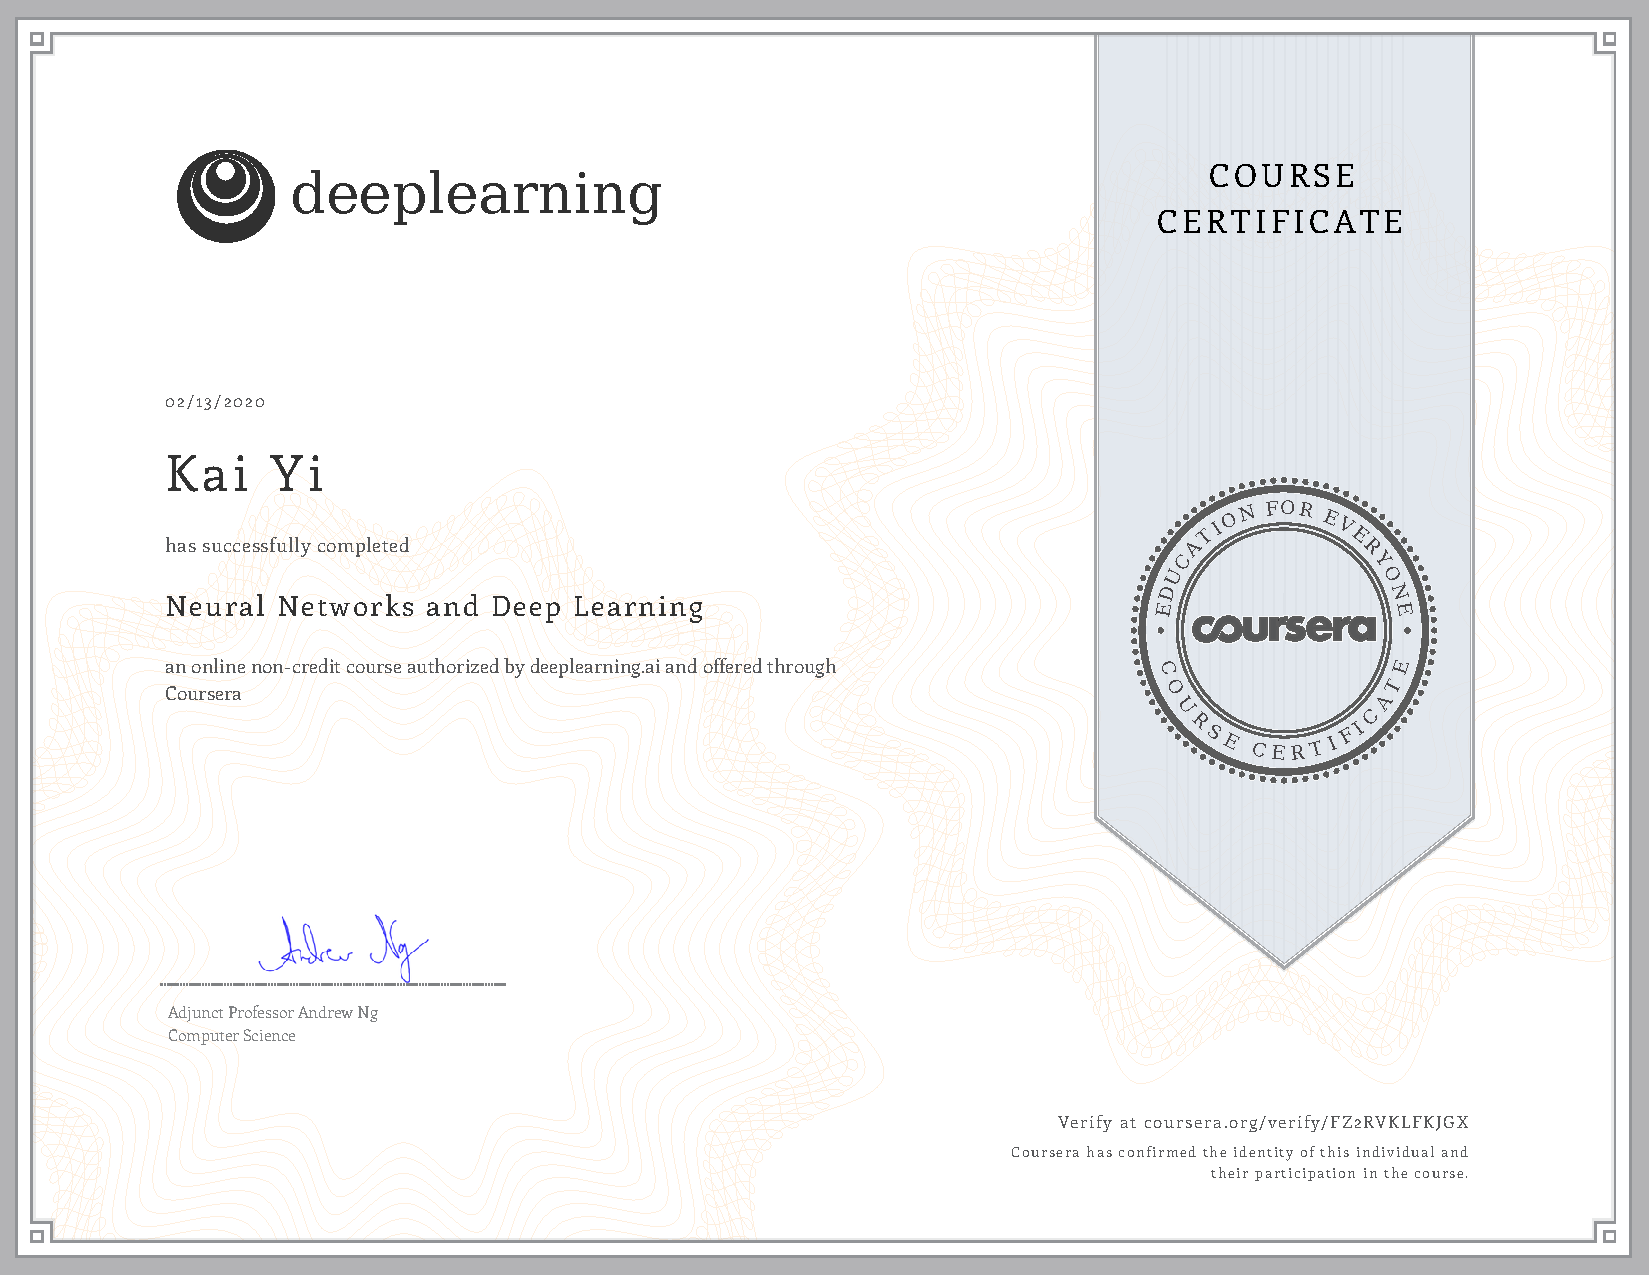
\includegraphics[width=1.0\textwidth]{img/C1-Certificate.pdf}
    \caption{Certificate of Neural Networks and Deep Learning. Obtained in Feb. 2020.}
    \label{C1-Certificate}
\end{figure}

\subsection{Course Overview}
According to the official site of this course, you will learn the foundations of deep learning. When you finish this course, you will:

\begin{itemize}
    \item Understand the major technology trends driving deep learning.
    \item Be able to build, train and apply fully connected deep neural networks.
    \item Know how to implement efficient (vectorized) neural networks.
    \item Understand the key parameters in a neural network's architecture.
\end{itemize}

\subsection{Introduction to Deep Learning}
The section will mainly talk about the major trends driving the rise of deep learning, and understand where and how it is applied today. As I'm very familiar with this part, so I will summarize the background briefly.

Why is deep learning taking off? Data, Computation and Algorithm.

\subsection{Neural Network Basics}
\subsubsection{Logistic Regression}
Algorithm is used for classifications with 2 classes.

$y = w^T x + b$ or $y = sigmoid (w^T x + b)$ if we need y to be in between 0 and 1 (probability).

\subsubsection{Logistic Regression Cost Function}
We don't use square root error ($L(\hat{y}, y) = \frac{1}{2} (\hat{y}- y)^2$) because it leads us to optimization problem which is non=convex, means it contains local optimum points. We are using cross-entropy loss like $L(\hat{y}, y) = - (y\log(\hat{y}) + (1-y)\log(1-\hat{y})$.

To explain the last function lets see:
\begin{itemize}
    \item If $y = 1 \to L(\hat{y},1) = -\log(\hat{y}) \to$ we want $\hat{y}$ to be the largest $\to \hat{y}$ biggest value is 1.
    \item If $y = 0 \to L(\hat{y},0) = -\log(1-\hat{y}) \to$ we want $1-\hat{y}$ to be the largest $\to \hat{y}$ to be smaller as possible because it can only has 1 value.
\end{itemize}

Then the cost function will be: $J(w, b) = \frac{1}{m} \sum(\hat{y}^{(i)}, y^{(i)})$. The cost function is the average of the loss of the entire training set.

\subsubsection{Gradient Descent}
The actual equations we will implement:

\begin{itemize}
    \item $w = w - \alpha dw$ (how much the function slopes in the w direction).
    \item $b = b - \alpha db$ (how much the function slopes in the b direction).
\end{itemize}

$dw$ represents $\frac{dJ(w,b)}{dw}$.

\subsubsection{Logistic Regression Gradient Descent}
In the video, Prof. Andrew discussed the derivatives of gradient descent example for one sample with two features $x1$ and $x2$ (Figure \ref{logistic-regression}).

\begin{figure}[!htbp]
    \centering
    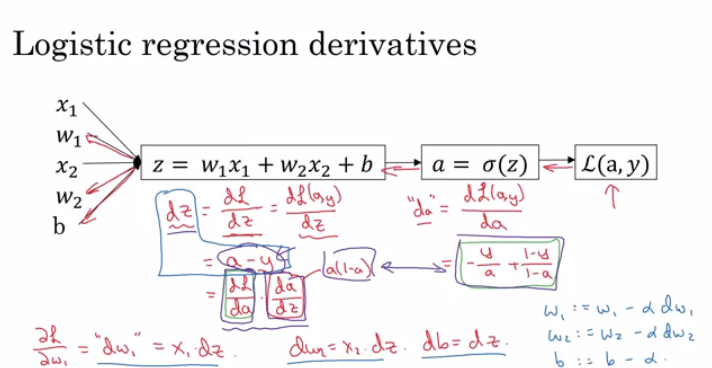
\includegraphics[width=1.0\textwidth, trim={0 0 0 50}, clip]{img/c1/logistic-regression.png}
    \caption{Logistic regression derivatives.}
    \label{logistic-regression}
\end{figure}

\subsubsection{Gradient Descent on m Examples}
The logistic regression pseudo code:

\begin{lstlisting}[language=python]
J = 0; dw1 = 0; dw2 =0; db = 0;     # Devs.
w1 = 0; w2 = 0; b=0;				# Weights
for i = 1 to m
	# Forward pass
	z(i) = W1*x1(i) + W2*x2(i) + b
	a(i) = Sigmoid(z(i))
	J += (Y(i)*log(a(i)) + (1-Y(i))*log(1-a(i)))

	# Backward pass
	dz(i) = a(i) - Y(i)
	dw1 += dz(i) * x1(i)
	dw2 += dz(i) * x2(i)
	db  += dz(i)
J /= m
dw1/= m
dw2/= m
db/= m

# Gradient descent
w1 = w1 - alpha * dw1
w2 = w2 - alpha * dw2
b = b - alpha * db
\end{lstlisting}

The above code should run for some iterations to minimize the error. So there will be two inner loops to implement the logistic regression.

Vectorization is so important on deep learning to reduce loops. In the last code we can make the whole loop in one step using vectorization!

\subsubsection{Vectorization}
Deep learning shines when the dataset are big. However for loops will make you wait a lot for a result. Thats why we need vectorization to get rid of some of our for loops.

NumPy library (dot) function is using vectorization by default. Most of the NumPy library methods are vectorized version.

The vectorization can be done on CPU or GPU thought the SIMD operation. But its faster on GPU.

Whenever possible avoid for loops.

\subsubsection{Vectorizing Logistic Regression}
As an input we have a matrix $X$ and its $[n_x, m]$ and a matrix Y and its $[n_y, m]$.

Thus we have:

\begin{lstlisting}[language=python]
Z = np.dot(W.T,X) + b  # Vectorization, then broadcasting, Z shape is (1, m)
A = 1 / 1 + np.exp(-Z) # Vectorization, A shape is (1, m)
\end{lstlisting}

Vectorizing Logistic Regression's Gradient Output:

\begin{lstlisting}[language=python]
dz = A - Y                  # Vectorization, dz shape is (1, m)
dw = np.dot(X, dz.T) / m    # Vectorization, dw shape is (n_x, 1)
db = dz.sum() / m           # Vectorization, dz shape is (1, 1)
\end{lstlisting}

\subsubsection{Notes on Python and Numpy}
In Numpy, obj.sum(axis = 0) sums the columns while obj.sum(axis = 1) sums the rows.

In Numpy, obj.reshape(1,4) changes the shape of the matrix by broadcasting the values.

Reshape is cheap in calculations so put it everywhere you're not sure about the calculations.

Broadcasting works when you do a matrix operation with matrices that doesn't match for the operation, in this case Numpy automatically makes the shapes ready for the operation by broadcasting the values.

In general principle of broadcasting. If you have an (m,n) matrix and you add(+) or subtract(-) or multiply(*) or divide(/) with a (1,n) matrix, then this will copy it m times into an (m,n) matrix. The same with if you use those operations with a (m , 1) matrix, then this will copy it n times into (m, n) matrix. And then apply the addition, subtraction, and multiplication of division element wise.

Some tricks to eliminate all the strange bugs in the code:

\begin{itemize}
    \item If you didn't specify the shape of a vector, it will take a shape of (m,) and the transpose operation won't work. You have to reshape it to (m, 1).
    \item Try to not use the rank one matrix in ANN.
    \item Don't hesitate to use assert(a.shape == (5,1)) to check if your matrix shape is the required one.
    \item If you've found a rank one matrix try to run reshape on it.
\end{itemize}

Jupyter / IPython notebooks are so useful library in python that makes it easy to integrate code and document at the same time. It runs in the browser and doesn't need an IDE to run.

To open Jupyter Notebook, open the command line and call: jupyter-notebook It should be installed to work.

To Compute the derivative of Sigmoid:
\begin{lstlisting}[language=python]
s = sigmoid(x)
ds = s * (1 - s)       # derivative  using calculus
\end{lstlisting}

To make an image of (width,height,depth) be a vector, use this:

\begin{lstlisting}[language=python]
v = image.reshape(image.shape[0]*image.shape[1]*image.shape[2],1) # reshapes the image.
Gradient descent converges faster after normalization of the input matrices.
\end{lstlisting}

\subsubsection{General Notes}
The main steps for building a Neural Network are:
\begin{itemize}
    \item Define the model structure (such as number of input features and outputs).
    \item Initialize the model's parameters.
    \item Loop. 1) Calculate current loss (forward propagation); 2) Calculate current gradient (backward propagation); 3) Update parameters (gradient descent).
\end{itemize}

Preprocessing the dataset is important.

Tuning the learning rate (which is an example of a "hyperparameter") can make a big difference to the algorithm.

% kaggle.com is a good place for datasets and competitions.


\subsection{Shallow Neural Networks}
In this section, you will learn to build a neural network with one hidden layer, using forward propagation and backpropagation.

\subsubsection{Neural Networks Overview}
In logistic regression we have:

\begin{lstlisting}
X1  \  
X2   ==>  z = WX + b ==> a = Sigmoid(z) ==> L(a,Y)
X3  /
\end{lstlisting}

In neural networks with one layer we will have:

\begin{lstlisting}
X1  \  
X2   =>  z1 = W1X + B1 => a1 = Sigmoid(z1) => z2 = W2a1 + B2 => 
         a2 = Sigmoid(z2) => L(a2,Y)
X3  /
\end{lstlisting}

\subsubsection{Neural Network Representation}
We will define the neural networks that has one hidden layer.

NN contains of input layers, hidden layers, output layers.

Hidden layer means we can't see that layers in the training set.

a0 = x (the input layer)

a1 will represent the activation of the hidden neurons.

a2 will represent the output layer.

We are talking about 2 layers NN. The input layer isn't counted.

\subsubsection{Computing a Neural Network's Output}
Equation of hidden layers (Figure \ref{nn-figure}):

\begin{figure}[!htbp]
    \centering
    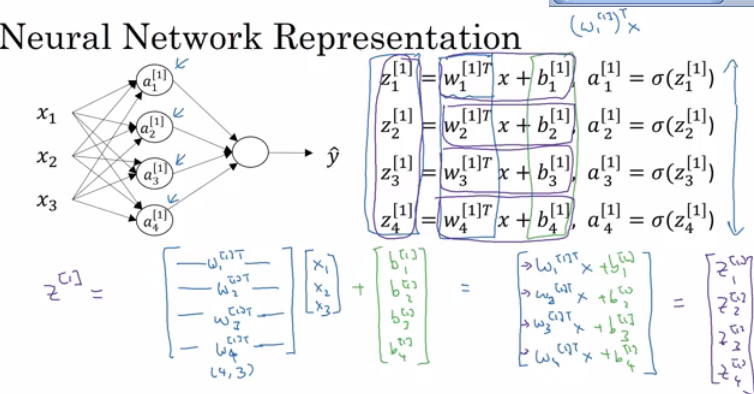
\includegraphics[width=1.0\textwidth, trim={0 0 0 50}, clip]{img/c1/nn-figure.png}
    \caption{Neural Network Representation.}
    \label{nn-figure}
\end{figure}

Shapes of variables:

\begin{itemize}
    \item $w^{[1]}: (n_h, n_x)$, $b^{[1]}: (n_h, 1)$, $z^[1] \to w^{[1]} X + b: (n_h, 1)$, $a^{[1]} \to g(z^{[1]}): (n_h, 1)$.
    \item $w^{[2]}: (1, n_x)$, $b^{[2]}: (1, 1)$, $z^[2] \to w^{[2]} a^{[1]} + b: (1, 1)$, $a^{[2]} \to g(z^{[2]}): (1, 1)$.
\end{itemize}

% Check whether its true.
% Others refer to the assignments for more information.

\subsubsection{Simple Neural Network}
Here is the neural network with a single hidden layer (Figure \ref{classification-kiank}):

\begin{figure}[!htbp]
    \centering 
    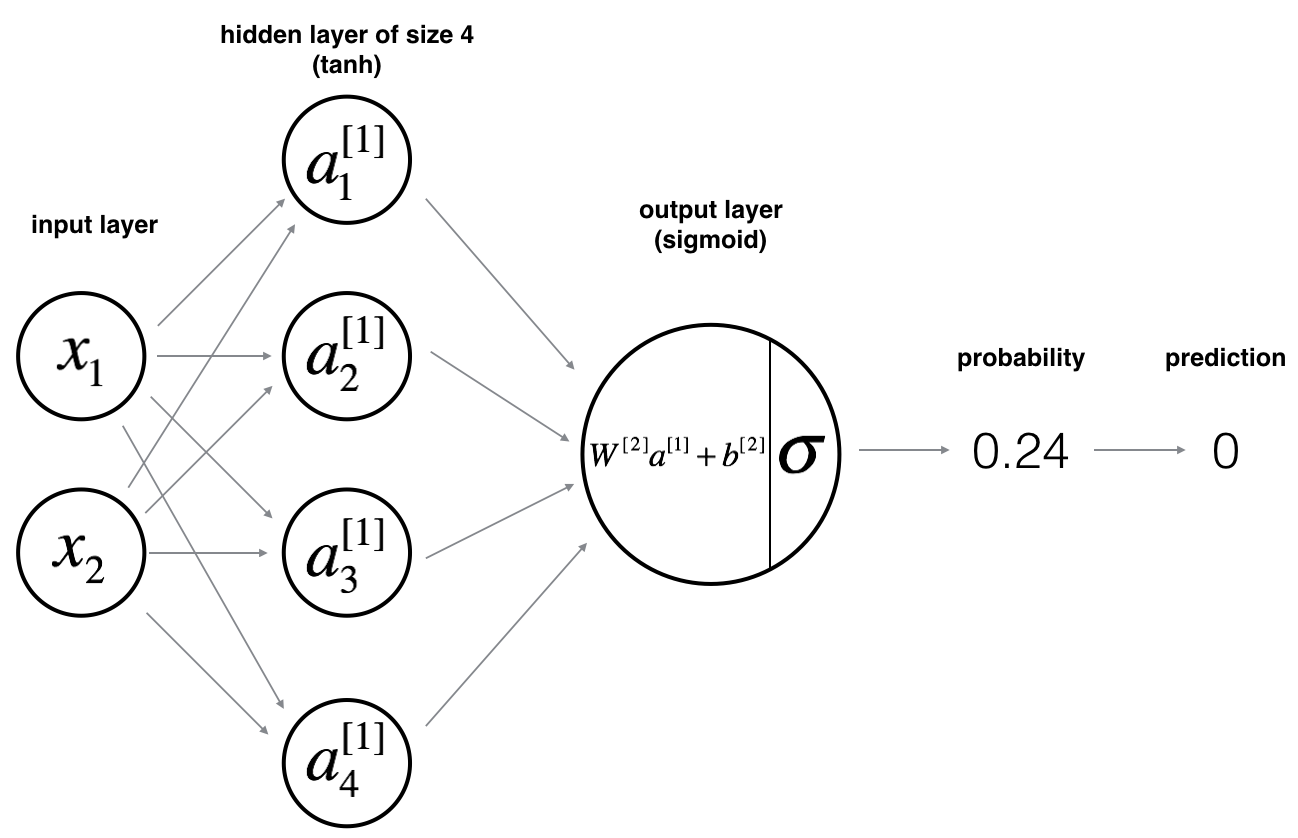
\includegraphics[width=0.8\textwidth, trim={0 0 0 0}, clip]{img/c1/classification_kiank.png}
    \caption{Network architecture with single hidden layer.}
    \label{classification-kiank}
\end{figure}

Mathematically, for one example $x^(i)$, we have: 

\begin{equation}
\centering
\begin{aligned}
z^{[1](i)}&=W^{[1]} x^{(i)}+b^{[1]} \\
a^{[1](i)}&=\tanh \left(z^{[1](i)}\right) \\
z^{[2](i)}&=W^{[2]} a^{[1](i)}+b^{[2]} \\
\hat{y}^{(i)}&=a^{[2](i)}=\sigma\left(z^{[2](i)}\right) \\
y^{(i)}_{\text {prediction}}&=\left\{\begin{array}{ll}
1 & \text { if } a^{[2](i)}>0.5 \\
0 & \text { otherwise }
\end{array}\right.
\end{aligned}
\end{equation}

Given the predictions on all the examples, you can also compute the cost $J$ as follows:

\begin{equation}
    J=-\frac{1}{m} \sum_{i=0}^{m}\left(y^{(i)} \log \left(a^{[2](i)}\right)+\left(1-y^{(i)}\right) \log \left(1-a^{[2](i)}\right)\right)
\end{equation}

The general methodology to build a neural network is to:

\begin{itemize}
    \item[i.]  Define the neural network structure (number of input units, number of hidden units, etc).
    \item[ii.] Initialize the model's parameters.
    \item[iii.] Loop: 1) Implement forward propagation; 2) Compute loss; 3) Implement backward propagation to get the gradients; 4) Update parameters (gradient descent).
\end{itemize}

\subsubsection{Gradient of NN with One Hidden Unit}
Here is the updating rules for the neural network with one hidden unit (Figure \ref{grad-summary}):

\begin{figure}[!htbp]
    \centering 
    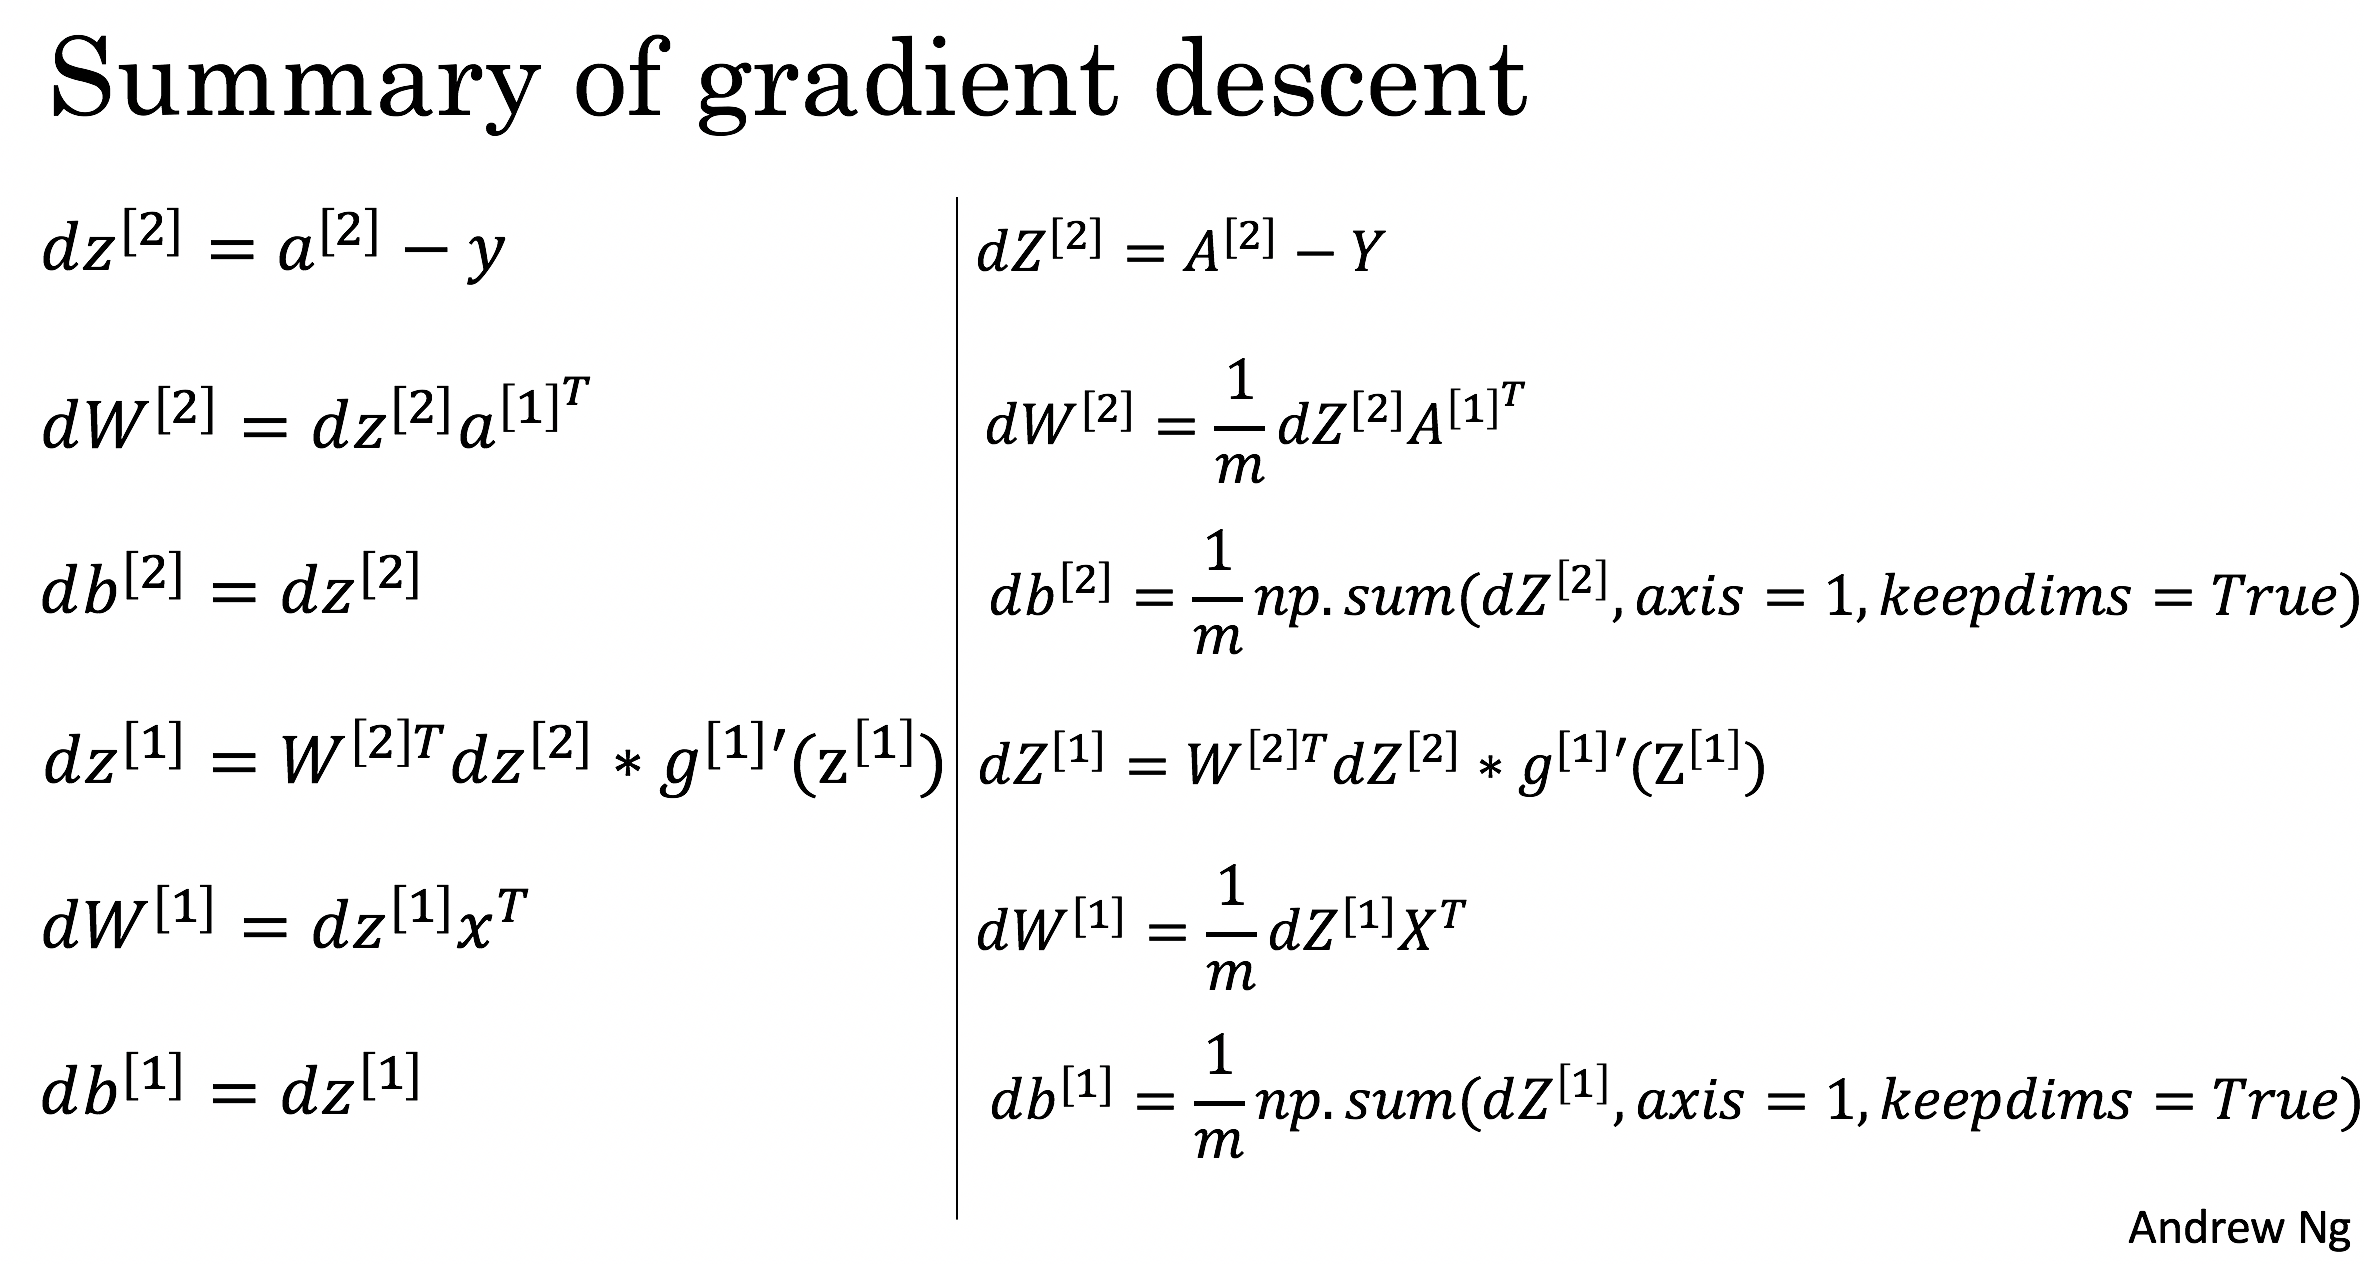
\includegraphics[width=1.0\textwidth, trim={0 0 0 60}, clip]{img/c1/grad_summary.png}
    \caption{Summary of gradient descent.}
    \label{grad-summary}
\end{figure}


\subsection{Deeper Neural Networks}
As the pipeline for deeper neural network is very similar to shallow neural network, so I will summarize this part briefly.

\subsubsection{Building Your Deeper Neural Network: Step by Step}
The pipeline of parameters updating (Figure \ref{final-outline}):

\begin{figure}[!htbp]
    \centering 
    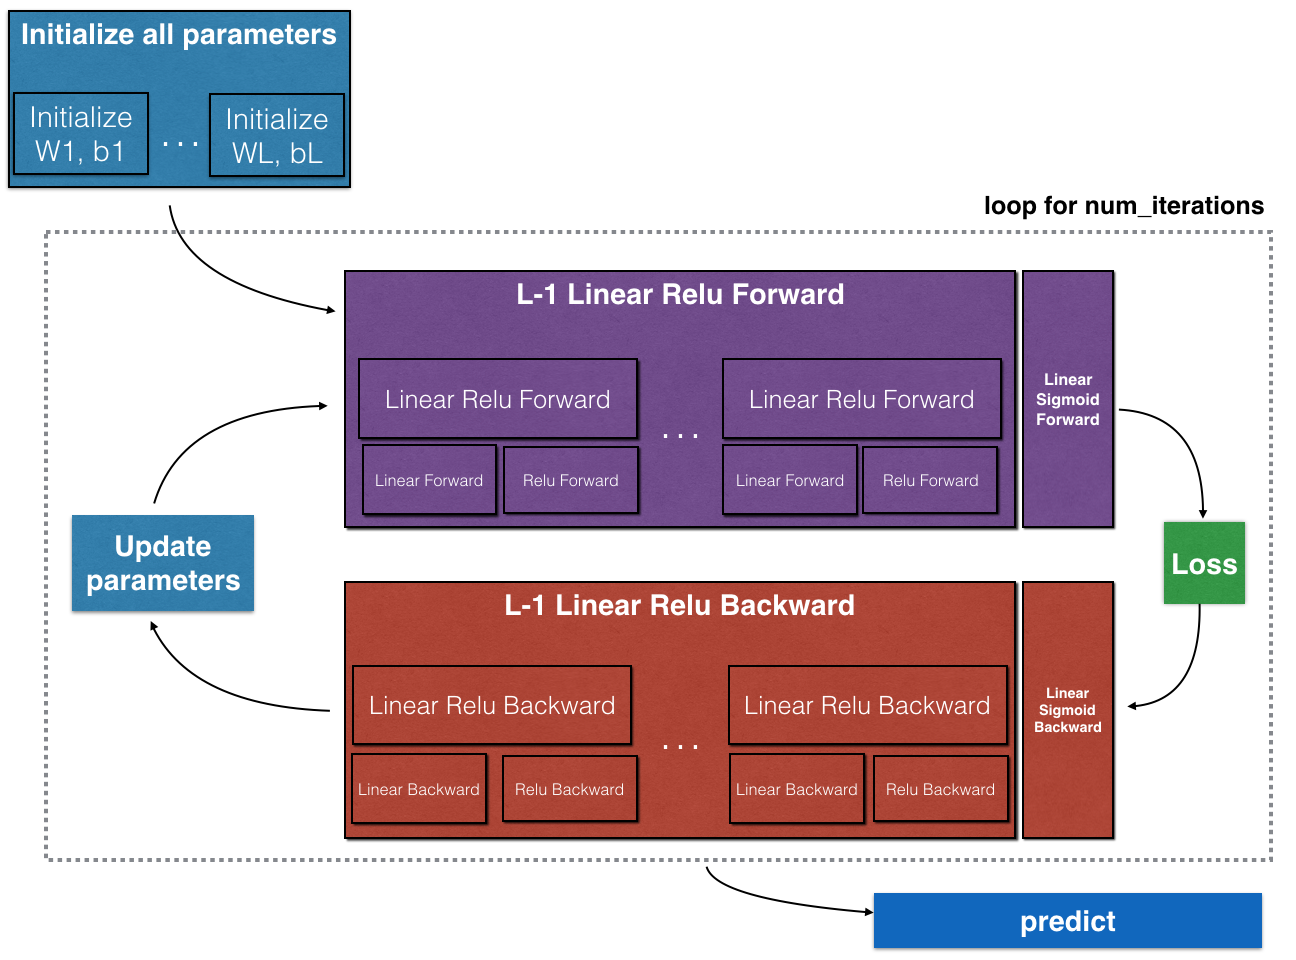
\includegraphics[width=1.0\textwidth, trim={0 0 0 0}, clip]{img/c1/final outline.png}
    \caption{The pipeline of parameters updating.}
    \label{final-outline}
\end{figure}

\paragraph{Forward Propagation}
The linear forward module (vectorized over all the examples) computes the following equations:

\begin{equation}
    Z^{[l]} = W^{[l]}A^{[l-1]} + b^{[l]}
\end{equation}

where $A^{[0]} = X$.

\paragraph{Cost Function}
\begin{equation}
    -\frac{1}{m} \sum_{i=1}^{m}\left(y^{(i)} \log \left(a^{[L](i)}\right)+\left(1-y^{(i)}\right) \log \left(1-a^{[L](i)}\right)\right)
\end{equation}

\paragraph{Illustrations of forward and backward propagation} Could refer to Figure \ref{backprop-kiank}.

\begin{figure}[!htbp]
    \centering 
    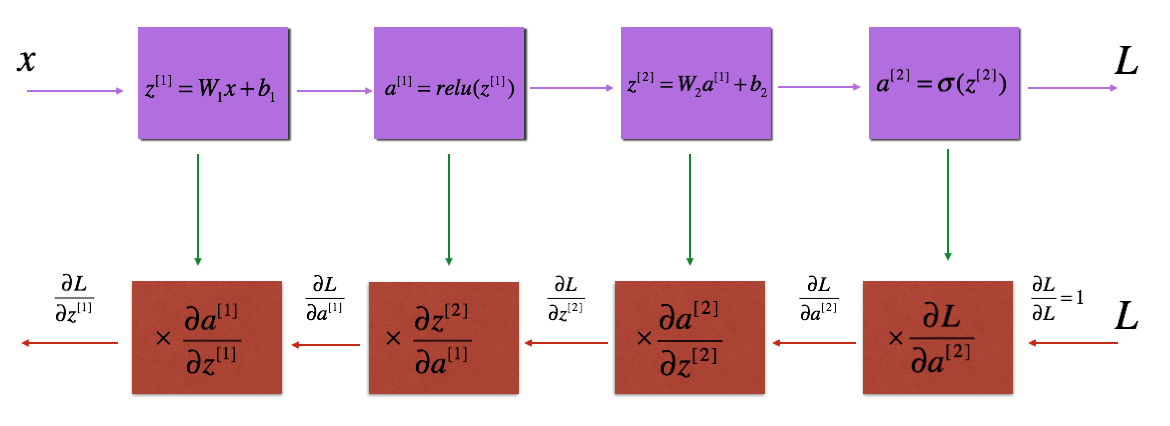
\includegraphics[width=1.0\textwidth, trim={0 0 0 0}, clip]{img/c1/backprop_kiank.png}
    \caption{Forward and Backward propagation for LINEAR->RELU->LINEAR->SIGMOID. The purple blocks represent the forward propagation, and the red blocks represent the backward propagation.}
    \label{backprop-kiank}
\end{figure}

\paragraph{Backward Gradients}
Here are the gradients for layer $l$:
\begin{equation}
\begin{aligned}
d W^{[l]} &=\frac{\partial \mathcal{J}}{\partial W^{[l]}}=\frac{1}{m} d Z^{[l]} A^{[l-1] T} \\
d b^{[l]} &=\frac{\partial \mathcal{J}}{\partial b^{[l]}}=\frac{1}{m} \sum_{i=1}^{m} d Z^{[l](i)} \\
d A^{[l-1]} &=\frac{\partial \mathcal{L}}{\partial A^{[l-1]}}=W^{[l] T} d Z^{[l]}
\end{aligned}
\end{equation}

\paragraph{Update Parameters}:

\begin{equation}
W^{[l]}=W^{[l]}-\alpha d W^{[l]} \\
b^{[l]}=b^{[l]}-\alpha d b^{[l]} \\
\end{equation}



\newpage
\section{Improving Deep Neural Networks: Hyperparameter tuning, Regularization and Optimization}
This is the second courseof deep learning specialization at Coursera taught by Professor Andrew Ng. Here is my certificate after finishing this course (Fig. \ref{course2-cert}):

\begin{figure}[!htbp]
    \centering
    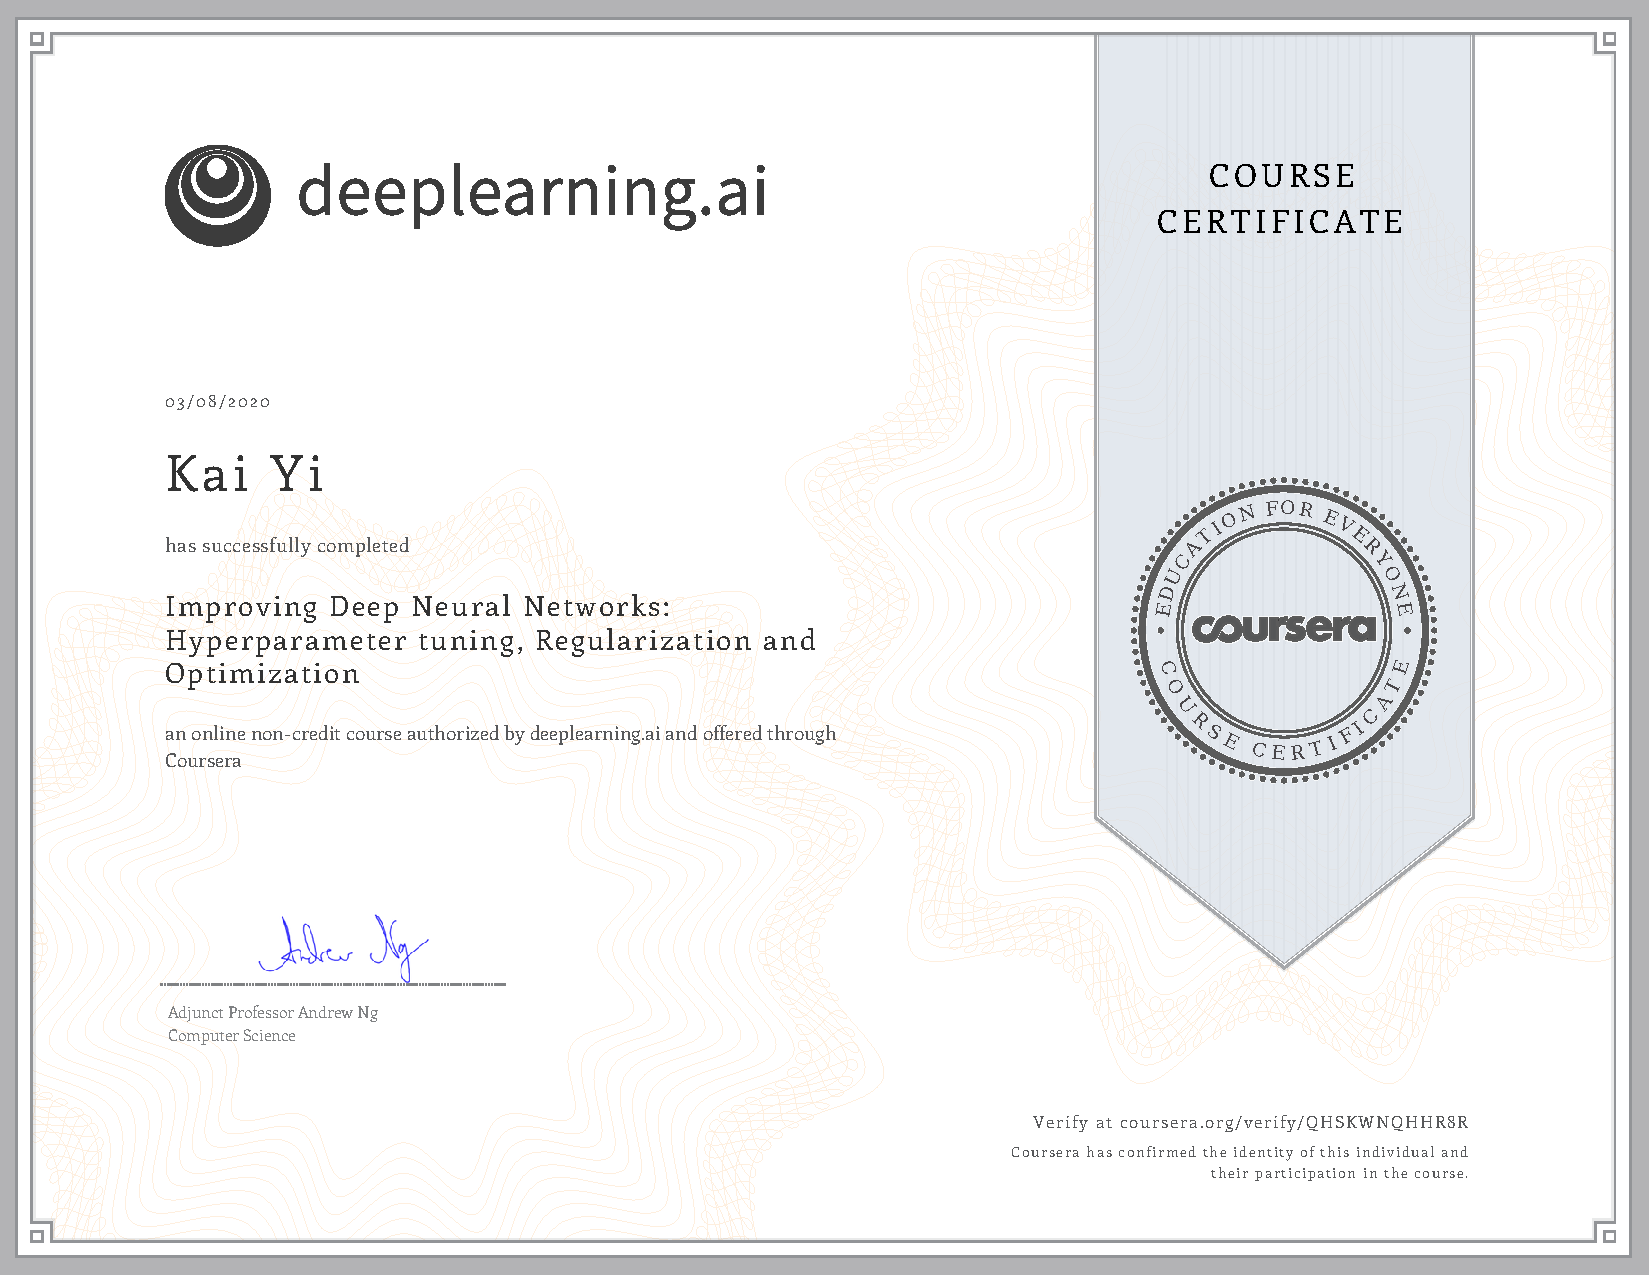
\includegraphics[width=1.0\textwidth]{img/C2-Certificate.pdf}
    \caption{Certificate of Improving Deep Neural Networks: Hyperparameter tuning, Regularization and Optimization. Obtained in March 2020.}
    \label{course2-cert}
\end{figure}

\subsection{Course Overview}
According to the official site of this course, there are following key components:

\begin{itemize}
    \item Understand industry best-practices for building deep learning applications.
    \item Be able to effectively use the common neural network 'tricks', including initialization, L2 and dropout regularization, batch normalization and gradient checking.
    \item Be able to implement and apply a variety of optimization algorithms, such as mini-batch gradient descent, momentum, RMSprop and Adam, and check for their convergence.
    \item Understand new best-practices for the deep learning era of how to set up train/dev/test sets and analyze bias/variance.
    \item Be able to implement a neural network in TensorFlow.
\end{itemize}

\subsection{Practical Aspects of Deep Learning}
\subsubsection{Train/Dev/Test Sets}
Pipeline of deep learning practice: Idea $>>$ Code $>>$ Experiment $>>$ Idea. We get initial idea first, then implement the rough idea. Next fine tuning our model based on experiment. Then we get new thoughts.

Data will be split into three parts:

\begin{itemize}
    \item Training Set. (the largest set)
    \item Hold-Out Cross Validation Set / Development Set.
    \item Test Set.
\end{itemize}

We will try to build a model upon training set then try to optimize hyperparameters on dev set as much as possible. Then after our model is ready we try and evaluate the testing set.

Thus the trend on the ratio of splitting the models:
\begin{itemize}
    \item If size of the dataset is 100 to 1,000,000, then $=>$ 60/20/20.
    \item If size of the dataset is more than 1,000,000, then $=>$ 98/1/1 or 99.5/0.25/0.25.
\end{itemize}

Make sure the dev and test set are coming from the same distribution. 

\begin{itemize}
    \item E.g. The cat training pictures from the web can be put into training set to get more data. However, the picture from users cell phone and the web have different distribution. Therefore, the web picture can not be used separately on dev set or test set. Besides, it's better not to use a little web picture on dev/test set (it will cause mismatch problem). Besides, 
\end{itemize}

It's OK to only have a dev set without a testing set. But a lot of people in this case call the dev set as the test set. A better terminology is to call it a dev set as its used in the development.

\subsubsection{Bias / Variance}
Bias / Variance techniques are easy to learning, but difficult to master.

\begin{itemize}
    \item Underfitting $=>$ High Bias
    \item Overfitting $=>$ High Variance
\end{itemize}

The following visualization (Fig. \ref{bias-variance}):

\begin{figure}
    \centering
    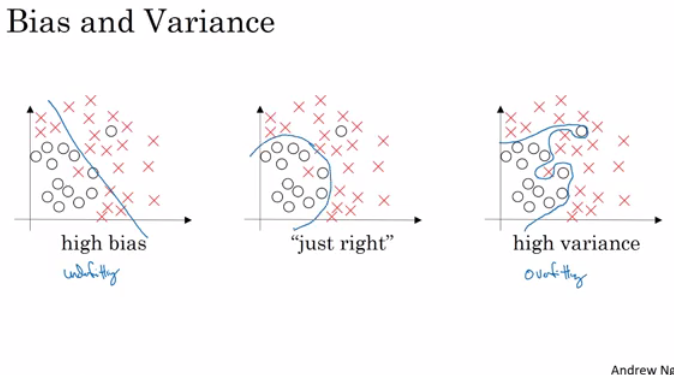
\includegraphics[width=1.0\textwidth, trim={0 70, 0 60}, clip]{img/c2/bias-variance.png}
    \caption{Bias and Variance.}
    \label{bias-variance}
\end{figure}

If Bayesian error (optimal error) is 0\%, next is several cases:

\begin{itemize}
    \item High variance (overfitting): Train error: 1\%, Dev error: 15\%
    \item High bias (underfitting): Train error: 10\%, Dev error: 8\%
    \item High bias \& high variance: Train error: 16\%, Dev error: 30\%
    \item Quite well: Train error: 0.6\%, Dev error: 0.9\%
\end{itemize}

\subsubsection{Basic Recipe for Machine Learning}
If my algorithm has a high bias:
\begin{itemize}
    \item Try to make my NN bigger (size of hidden units, number of layers).
    \item Try to train it longer.
    \item (Not unique) Try a different model that is suitable for my data / Try different (advanced) optimization algorithms.
\end{itemize}

If my algorithm has a high variance:
\begin{itemize}
    \item Get more data.
    \item Try regularization.
    \item (Not unique) Try a different model that is suitable for my data / Try different (advanced) optimization algorithms.
\end{itemize}

I should try the previous two points until I have a low bias and low variance.

In the older days before deep learning, there was a 'Bias/Variance Tradeoff'. But nowadays we can reduce bias and variance separately by using more advanced tools and techniques.

\subsubsection{Regularization}
Adding regularization to NN will help it reduce variance (overfitting).

\begin{itemize}
    \item L1 matrix norm: $||W|| = \sum w_{ij}$.

    \item L2 matrix norm: $||W||^2 = \sum w_{ij}^2$. Also $||W||^2 = W^T * W $ if W is a vector.
\end{itemize}

Regularization for logistic regression: (Find more accurate equations for regularizations)
\begin{itemize}
    \item The normal cost function that we want to minimize is: $J(W, b) = \frac{1}{m} \sum L(y_i, \hat{y}_i)$
    \item The L2 regularization version: $J(W,b) = \frac{1}{m} \sum L(y_i, \hat{y}_i) + \frac{\lambda}{2m} \sum w_i^2$
    \item The L1 regularization version: $J(W,b) = \frac{1}{m} \sum L(y_i, \hat{y}_i + \frac{\lambda}{m} \sum w_i$
    \item L2 regularization is being used much more often and $\lambda$ here is the regularization parameter (hyperparameter)
\end{itemize}

(Some points I can not understand very clearly here.)
% https://github.com/mbadry1/DeepLearning.ai-Summary/tree/master/2-%20Improving%20Deep%20Neural%20Networks

\subsubsection{Why regularization reduces overfitting?}
Here are som intuitions:

Intuition 1:
\begin{itemize}
    \item If $\lambda$ is too large - a lot of w's will be close to zeros which will make the NN simpler (I can think of it as it would behave closer to logistic regression).
    \item If $\lambda$ is good enough it will just reduce some weights that makes the neural network overfit.
\end{itemize}

Intuition2 (with tanh activation function):
\begin{itemize}
    \item If $\lambda$ is too large, w's will be small (close to zero) - will use the linear part of the tanh activation function, so we will go from non linear activation to roughly linear which would make the NN a roughly linear classifier.
    \item If $\lambda$ is good enought, it will just make some of tanh activations roughly linear which will prevent overfitting.
\end{itemize}

Implementation tip: if you implement gradient descent, one of the steps to debug gradient descent is to plot the cost function J as a function of the number of iterations of gradient descent and you want to see that the cost function J decreases monotonically after every elevation of gradient descent with regularization. If you plot the old definition of J (no regularization) then you might not see it decrease monotonically.

\subsubsection{Dropout Regularization}
The dropout regularization eliminates some neurons/weights on each iteration based on a probability. A most common technique to implement dropout is called "inverted dropout".

Code for inverted dropout:

\begin{lstlisting}[language=python]
keep_prob = 0.8 # 0 <= keep_prob <= 1, this code is only for layer 3

# the generated number that are greater than keep_prob will be 
# dropped. Thus 80% stay, 20% dropped.
# a3.shape = (num_neurons l3, m examples)
d3 = np.random.rand(a3.shape[0], a[l].shape[1]) < keep_prob

a3 = np.multiply(a3, d3) # only keep the values in d3 (True)

a3 = a3 / keep_prob # re-scaling a3, inverted dropout.
\end{lstlisting}

Matrix d3 is used for forward and back propagation and is the same for them, but it is different for each iteration due to the random initialization.

At test time we don't use dropout. If I implement dropout at test time - it would add noise to predictions.

\subsubsection{Understanding Dropout}
Intuition 1:
\begin{itemize}
    \item The intuition was that dropout randomly knocks out units in my network. So it's as if on every iteration I'm working with a smaller NN, and so using a smaller NN seems like it should have a regularizing effect.
\end{itemize}

Intuition 2:
\begin{itemize}
    \item NN can't rely on any one feature, so it has to spread out weights.
\end{itemize}

Dropout can have different keep\_prob per layer. And the input layer dropout has to be near 1 because I don't want to eliminate a lot of features.

A lot of researchers are using dropout in the area of computer vision because they have a very big input size and almost never have enough data, so overfitting is the usual problem. And dropout is a regularization technique to prevent overfitting.

A downside of dropout is that the cost function J is not well defined and it will be hard to debug (plot J by iteration).
\begin{itemize}
    \item To solve that I'll need to turn off dropout, set all the keep\_prob s to 1, and then run the code and check that it monotonically decreases J and then turn on the dropouts again.
\end{itemize}

\subsubsection{Other regularization methods}
\paragraph{Data Augmentation}
For example in a computer vision task:

\begin{itemize}
    \item Flip all my pictures horizontally which will give my more data instances
    \item Apply a random position and rotation to an image to get more data.
\end{itemize}

New data obtained using this technique isn't as good as the real independent data, but still can be used as a regularization technique.

\paragraph{Early Stopping}
In this technique we plot the training set and the dev set cost together for each iteration. At some iteration the dev set cost will top decreasing and will start increasing. 

We will pick the point at which the training set error and dev set error are best (great trade-off between dev error and train error). Thus we can take these parameters as the best parameters (Visualized at Fig. \ref{early-stopping}).

\begin{figure}[!htbp]
    \centering
    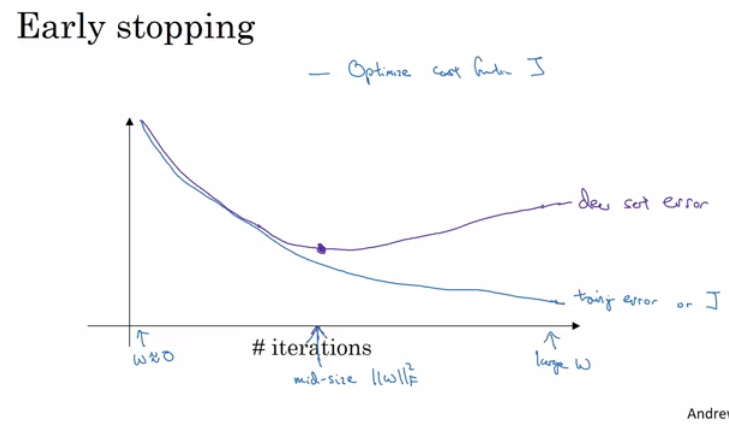
\includegraphics[width=1.0\textwidth, trim={30 30, 0 90}, clip]{img/c2/early-stopping.png}
    \caption{Early stopping method preventing overfitting.}
    \label{early-stopping}
\end{figure}

Professor Andrew prefers to use L2 regularization instead of early stopping because this technique simultaneously tries to minimize the cost function and not to overfit which contradicts the orthogonalization approach (we should not make decision on two variables).

However, the advantage of early stopping is that we don't need to search a hyperparameter like in other regularization approaches (like $\lambda$ in L2 regularization).

\paragraph{Model Ensembles}
Basic idea: Train multiple independent models and at test time average their results.

It can get 2\% improved performance and can be used in competitions instead of practical deployments. It reduces the generalization error. 

\subsubsection{Normalizing Inputs}
If I normalize my inputs this will speed up the training process a lot (convert optimizing from ellipse to circular).

Normalization are going on these steps:

\begin{itemize}
    \item Get the mean of the training set: mean = (1/m) * sum(x(i))
    \item Subtract the mean from each input: X = X - mean. This makes my inputs centered around 0.
    \item Get the variance of the training set: variance = (1/m) * sum((x(i)-mean)**2)
    \item Normalize the variance: X /= variance
\end{itemize}

These steps should be applied to training, dev, and testing sets (but using mean and variance of the train set).

Why normalize?
\begin{itemize}
    \item If we don't normalize the inputs our cost function will be deep and its shape will be inconsistent (elongated) then optimizing it will take a long time.
    \item But if we normalize it the opposite will occur. The shape of the cost function will be consistent (look more symmetric like circle in 2D example) and we can use a larger learning rate $\alpha$ - the optimization will be faster.
\end{itemize}


\subsubsection{Vanishing / Exploding gradients}
The vanishing / exploding gradients occurs when our derivatives become very small or very big.

To understand the problem, suppose that we have a deep neural network with number of layer L, and all the activation functions are linear and each b=0.

Then $\hat{Y} = W[L]W[L-1]\cdot W[1]X$. If we have 2 hidden units per layer and x1=x2=1, if W[i,j] is greater than 1, then $\hat{Y}$ will be exponentially large. Meanwhile, if W[i,j] is smaller than 1, then $\hat{Y}$ will be exponentially small.

\subsubsection{Weight Initialization for Deep Networks}
A partial solutions to the vanishing / exploding gradients in NN is better or more careful choice of the random initialization of weights.

A well chosen initialization can:

\begin{itemize}
    \item Speed up the convergence of gradient descent
    \item Increase the odds of gradient descent converging to a lower training (and generalization) error.
\end{itemize}

\begin{itemize}
    \item Zero Initialization: \textit{np.zeros(shape)}
    \item Random Initialization: \textit{np.random.randn(shape} * 0.01
    \item Bengio et al. Initialization: \textit{np.random.randn(shape) * np.sqrt(2/(n[l-1] + n[l])}
    \item He et al. Initialization (Xavier Initialization): \textit{np.random.randn(shape) + np.sqrt(2/n[l-1])} (Set ReLu as activation is better)
\end{itemize}

\subsubsection{Numerical approximation of gradients}
There is a technique called gradient checking which tells you if your implementation of backpropagation is correct.

There is a numerical way to calculate the derivative (Fig. \ref{gradient-checking})

\begin{figure}
    \centering
    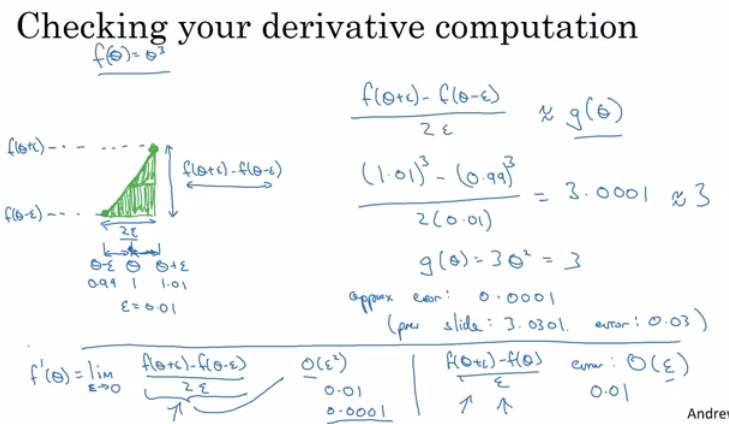
\includegraphics[width=1.0\textwidth, trim={0 0 0 35}, clip]{img/c2/gradient-checking.png}
    \caption{Checking the derivative computation.}
    \label{gradient-checking}
\end{figure}

Gradient checking is used only for debugging.

Main goal is to check whether the following satisfied:

\begin{equation}
    \frac{\partial J}{\partial \theta} = lim_{\epsilon \to 0}\frac{J(\theta + \epsilon) - J(\theta - \epsilon}{2\epsilon}
\end{equation}


% \begin{lstlisting}[language=python]
% epsilon = 1e-7
% for i in len(theta):
%     d_theta_approx[]
% \end{lstlisting}

% Adding more contents

\subsubsection{Gradient checking implementation notes}
Don't use the gradient checking algorithm at training time because it's very slow. Use gradient checking only for debugging. If algorithm fails grad check, look at components to try to identify the bug.

Don't forget to add $\frac{\lambda}{2m} \sum w_i$ to J if we're using L1 or L2 regularization.

Gradient checking doesn't work with dropout because J is not consistent. We must first turn off dropout, run gradient checking and then turn on dropout again.

Run gradient checking at random initialization and train the network for a while maybe there's a bug which can be seen when w's and b's become larger (further from 0) and can't be seen on the first iteration (when w's and b's are very small).

\subsubsection{Initialization Summary}
The weights should be initialized randomly to break symmetry.

It's OK to initialize the biases to zeros. Symmetry still can be broken so long as weights are initialized randomly.

Different initializations lead to different results.

Random initialization is used to break symmetry and make sure different hidden units can learn different things.

Don't initialize to values that are to large.

He initialization (Xavier Initialization) works well for networks with ReLU activations.

\subsubsection{Regularization Summary}
\paragraph{L2 Regularization}
The value of $\lambda$ is a hyperparameter that you can tune using a dev set. L2 regularization makes the decision boundary smoother. If $\lambda$ is too large, it's also possible to `oversmooth', resulting in a model with high bias.

\subparagraph{What is L2-regularization actually doing?} L2 regularization relies on the assumption that a model with large weights is simpler than one with small weights. Thus, by penalizing the square value of the weights in the cost function, you drive all the weights to smaller values. It becomes too costly for the cost to have large weights. This leads to a smoother model in which the output changes more slowly as the input changes.

\paragraph{Dropout}
Dropout is a regularization technique. You only use dropout during training. Don't use it (randomly eliminates nodes) during test time.

Apply dropout both during forward and backward propagation.

During training time, divide each dropout layer by keep\_prob to keep the same expected value for the activations. For example, if keep\_prob is 0.5, then we will on average shut down half the nodes, so the output will be scaled by 0.5 since only the remaining half are contributing to the solution. Dividing by 0.5 is equivalent to multiplying by 2. Hence, the output now has the same expected value. You can check that this works even when keep\_prob is other values than 0.5.

\newpage

\subsection{Optimization Algorithms}
% Continue to summarizing optimization algorithms.
% https://github.com/mbadry1/DeepLearning.ai-Summary/tree/master/2-%20Improving%20Deep%20Neural%20Networks#why-regularization-reduces-overfitting

\subsubsection{Mini-Batch Gradient Descent}
Training NN with large data is slow. So to find an optimization algorithm that runs faster is a good idea.

Suppose we have m = 50 million. To train this data it will take a huge processing time for one step. Because 50 million won't fit in the memory at once we need other processing to make such a thing.

In Batch Gradient Descent we run the gradient descent on the whole dataset while in Mini-Batch Gradient Descent we run the gradient descent on the mini datasets.

\begin{lstlisting}[language=python]
for t = 1:No_of_batches  # for every epoch
	AL, caches = forward_prop(X{t}, Y{t})
	cost = compute_cost(AL, Y{t})
	grads = backward_prop(AL, caches)
	update_parameters(grads)
\end{lstlisting}

The code inside an epoch should be vectorized. Mini-batch gradient descent works much faster in the large datasets.

\subsubsection{Understanding mini-batch gradient descent}
In mini-batch algorithm, the cost won't go down with each step as it does in batch algorithm. It could contain some ups and downs but generally it has to go down (unlike the batch gradient descent where cost function decreases on each iterations (Fig. \ref{mini-batch-gradient}).

\begin{figure}
    \centering
    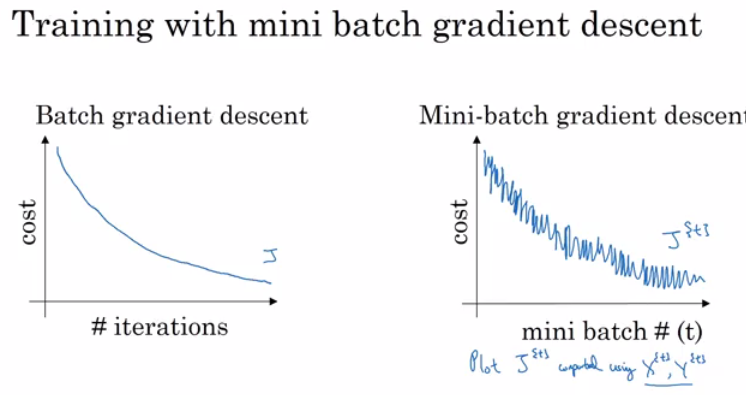
\includegraphics[width=1.0\textwidth, trim={0 35 0 70}, clip]{img/c2/batch_vs_mini_batch_cost.png}
    \caption{Training with mini batch gradient descent}
    \label{mini-batch-gradient}
\end{figure}

Mini-batch size:
\begin{itemize}
    \item (mini\_batch\_size = m) => batch gradient descent
    \item (mini\_batch\_size = 1) => stochastic gradient descent (SGD)
    \item (mini\_batch\_size =  between 1 and m) => ordinary mini-batch gradient descent
\end{itemize}

Batch gradient descent:
\begin{itemize}
    \item too long per iteration (epoch)
\end{itemize}

Stochastic gradient descent:
\begin{itemize}
    \item too noisy regarding cost minimization (can be reduced by using smaller learning rate)
    \item won't ever converge (reach the minimum cost)
    \item lose speedup from vectorization
\end{itemize}

Mini-batch gradient descent:
\begin{itemize}
    \item faster learning (you have the vectorization advantage and make progress without waiting to process the entire training set)
    \item doesn't always exactly converge (oscelates in a very small region, but you can reduce learning rate)
\end{itemize}

Guidelines for choosing mini-batch size:
\begin{itemize}
    \item If small training set (<2000 examples) - use batch gradient descent.
    \item It has to be a power of 2 (because of the way computer memory is layed out and accessed, somtimes your code runs faster if your mini-batch size is a power of 2): 64, 128, 256, 512, 1024, ...
    \item Make sure that mini-batch fits in CPU/GPU memory.
\end{itemize}

Mini-batch size is a hyperparameter.

\subsubsection{Exponentially weighted averages}
% Continue from \hyperref[here.]{https://github.com/mbadry1/DeepLearning.ai-Summary/tree/master/2-%20Improving%20Deep%20Neural%20Networks#exponentially-weighted-averages}.
There are optimization algorithms that are better than gradient descent, but you should first learn about Exponentially Weighted Averages.

If we have data like the temperature of day through the year it could be like this:

\begin{equation}
\begin{aligned}
\theta (1) & = 40\ \  (t(1) = 40)\\
\theta (2) &= 49\\
\theta (3) &= 45\\
&...\\
\theta (180) &= 60\\
&...
\end{aligned}
\end{equation}


This data is small in winter and big in summer. If we plot this data we will find it some noisy. 

Now lets computer the exponentially weighted averages:

\begin{equation}
    \begin{aligned}
    v0 &= 0\\
    v1 &= 0.9 * v0 + 0.1 * \theta(1) = 4\\
    v2 &= 0.9 * v1 + 0.1 * \theta(2) = 8.5\\
    v3 &= 0.9 * v2 + 0.1 * \theta(3) = 12.15\\
    &...
    \end{aligned}
\end{equation}

General equation:

\begin{equation}\label{ewa}
    v(t) = \beta v(t-1) + (1 - \beta) \theta (t)
\end{equation}

If we plot Equation \ref{ewa} it will represent averages over $ ~ \frac{1}{1-\beta}$ entries:

\begin{itemize}
    \item $\beta = 0.9$ will average last 10 entries
    \item $\beta = 0.98$ will average last 50 entries
    \item $\beta = 0.5$ will average last 2 entries
\end{itemize}

Best $\beta$ average for our case is between 0.9 and 0.98.

\paragraph{Intuition:} The reason why exponentially weighted averages are useful for further optimizing gradient descent algorithms is that it can give different weights to recent data points ($\theta$) based on value of $\beta$. If $\beta$ is high (around 0.9), it smoothens out the averages of skewed data points (oscillations w.r.t gradient descent terminology). So this reduces oscillations in gradient descent and hence makes faster and smoother path towards minimal (Fig \ref{ewa-example}).

\begin{figure}[!htbp]
    \centering
    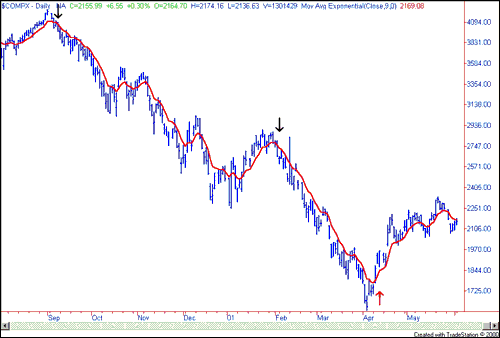
\includegraphics[width=0.8\textwidth]{img/c2/ewa.png}
    \caption{Visualization of exponentially weighted averages.}
    \label{ewa-example}
\end{figure}

\subsubsection{Bias correction in exponentially weighted averages}
The bias correction helps make the exponentially weighted averages more accurate. Because $v(0)=0$, the bias of the weighted averages is shifted and the accuracy suffers at the start.

To solve the bias issue we have to use this equation:

\begin{equation}
    v(t) = \frac{\beta v(t-1) + (1 - \beta) \theta(t)}{(1 - \beta^t)}
\end{equation}

As $t$ becomes larger, $1 - \beta^t$ becomes close to $1$.

\subsubsection{Gradient Descent With Momentum}
The momentum algorithm almost always works faster than standard gradient descent.

The simple idea is to calculate the exponentially weighted average for your gradients and then update your weights with the new values.

Here is the pseudo code:

\begin{lstlisting}[language=python]
vdW = 0, vdb = 0
on iteration t:
    # can be mini-batch or batch gradient descent
    # to compute dW, db on current batch
    
    vdW = beta * vdW + (1 - beta) * dW
    vdb = beta * vdb + (1 - beta) * db
    W = W - learning_rate * vdW
    b = b - learning_rate * vdb
\end{lstlisting}

Momentum helps the cost function to go to the minimum point in a more fast and consistent way.

$\beta$ is a hyperparameter . $\beta = 0.9$ is very common and works very well in most cases. In practice, people don't bother implementing bias correction.

\subsubsection{RMSprop (Root Mean Square prop)}
Here is the pseudo code:
\begin{lstlisting}[language=python]
sdW = 0, sdb = 0
sdW = 0, sdb = 0
on iteration t:
    # can be mini-batch or batch gradient descent
    # compute dw, db on current mini-batch
    
    sdW = (beta * sdW) + (1 - beta) * dW^2  # squaring is element-wise
    sdb = (beta * sdb) + (1 - beta) * db^2  # squaring is element-wise
    W = W - learning_rate * dW / sqrt(sdW)
    b = B - learning_rate * db / sqrt(sdb)
\end{lstlisting}

RMSprop will make the cost function move slower on the vertical direction and faster on the horizontal direction in the following example (Fig. \ref{rmsprop}):

\begin{figure}[!htbp]
    \centering
    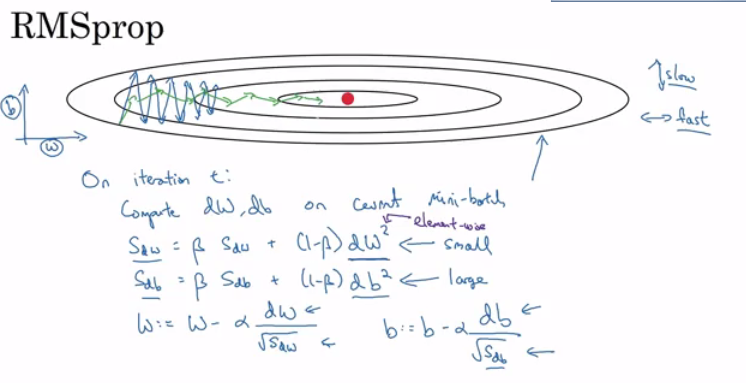
\includegraphics[width=1.0\textwidth, trim={0 0 0 33}, clip]{img/c2/RMSprop.png}
    \caption{Intuition of RMSprop.}
    \label{rmsprop}
\end{figure}

Ensure that $sdW$ is not zero by adding a small value $\epsilon$ (e.g. $\epsilon=10^{-8}$) to it ($\alpha$ represents the learning rate):

\begin{equation}
    W = W - \alpha * \frac{dW}{\sqrt{sdW + \epsilon}}
\end{equation}

With RMSprop you can increase your learning rate. Its developed by Geoffrey Hinton and firstly introduced on Coursera.org course (Neural Networks and Machine Learning).

\subsubsection{Adam Optimization Algorithm}
Stands for Adaptive Moment Estimation.

Adam optimization and RMSprop are among the optimization algorithms that worked very well with a lot of NN architectures.

Adam optimization simply puts RMSprop and momentum together.

Here is the pseudo code:

\begin{lstlisting}[language=python]
vdW = 0, vdW = 0
sdW = 0, sdb = 0
on iteration t:
	# can be mini-batch or batch gradient descent
	# to compute dw, db on current mini-batch                
			
	vdW = (beta1 * vdW) + (1 - beta1) * dW     # momentum
	vdb = (beta1 * vdb) + (1 - beta1) * db     # momentum
			
	sdW = (beta2 * sdW) + (1 - beta2) * dW^2   # RMSprop
	sdb = (beta2 * sdb) + (1 - beta2) * db^2   # RMSprop
			
	vdW = vdW / (1 - beta1^t)      # fixing bias
	vdb = vdb / (1 - beta1^t)      # fixing bias
			
	sdW = sdW / (1 - beta2^t)      # fixing bias
	sdb = sdb / (1 - beta2^t)      # fixing bias
					
	W = W - learning_rate * vdW / (sqrt(sdW) + epsilon)
	b = b - learning_rate * vdb / (sqrt(sdb) + epsilon)
\end{lstlisting}

Here is the equation form:

\begin{equation}
\centering
\begin{aligned}
    vdW &= (\beta_1 * vdW) + (1 - \beta_1) * dW\\
    vdb &= (\beta_1 * vdb) + (1 - \beta_1) * db\\
    sdW &= (\beta_2 * sdW) + (1 - \beta_2) * dW^2\\
    sdb &= (\beta_2 * sdb) + (1 - \beta_2) * db^2\\
    vdW &= vdW / (1 - \beta_1^t)\\
    vdb &= vdb / (1 - \beta_1^t)\\
    sdW &= sdW / (1 - \beta_2^t)\\
    sdb &= sdb / (1 - \beta_2^t)\\
    W &= W - \alpha * \frac{vdW}{\sqrt(sdW) + \epsilon}\\
    b &= b - \alpha * \frac{vdb}{\sqrt(sdW) + \epsilon}
\end{aligned}
\end{equation}

Hyperparameters for Adam:
\begin{itemize}
    \item Learning rate: needed to be tuned.
    \item $\beta_1$: parameter of the momentum - 0.9 is recommended by default.
    \item $\beta_2$: parameter of the RMSprop - 0.999 is recommended by default.
    \item $\epsilon$: $10^-8$ is recommended by default.
\end{itemize}

\subsubsection{Learning Rate Decay}
Slowly reduce learning rate.

As mentioned before mini-batch gradient descent won't reach the optimum point (converge). But by making the learning rate decay with iterations it will be much closer to it because the steps (and possible oscillations) near the optimum are smaller.

% One technique equation is \textit{learning\_rate = (1 / (1 + decay\_rate * epoch\_num)) * learning\_rate\_0}.

Several popular decay rate decay ($r$ represents the decay rate and i represents the current number of epoch):

\begin{equation}
    \begin{aligned}
        \alpha &= \frac{1}{1 + r * i} * \alpha_0\\
        \alpha &= 0.95^i * \alpha_0\\
        \alpha &= \frac{k}{\sqrt{i}} * \alpha_0
    \end{aligned}
\end{equation}

Besides, some people perform learning rate decay discretely - repeatedly decrease after some number of epochs. While also some people are making changes to the learning rate manually.

decay\_rate $r$  is another hyperparameter which has less priority.

\subsubsection{The Problem of Local Optima}
The normal local optima is not likely to appear in a deep neural network because data is usually high dimensional. For point to be a local optima it has to be a local optima for each of the dimensions which is highly unlikely.

It's unlikely to get stuck in a bad local optima in high dimensions, it is much more likely to get to the saddle point rather to the local optima, which is not a problem.

Plateaus can make learning slow:
\begin{itemize}
    \item Plateau is a region where the derivative is close to zero for a long time.
    \item This is where algorithms like momentum, RMSprop or Adam can help.
\end{itemize}

\subsection{Hyperparameter Tuning, Batch Normalization and Programming Frameworks}
\subsubsection{Tuning Process}
We need to tune our hyperparameters to get the best out of them.

Hyperparameters importance are (as for Andrew Ng, importance doesn't decrease strictly):

\begin{itemize}
    \item[i.] Learning rate
    \item[ii.] Momentum beta
    \item[iii.] Mini-batch size
    \item[iv.] No. of hidden units
    \item[v.] No. of layers
    \item[vi.] Learning rate decay
    \item[vii.] Regularization lambda
    \item[viii.] Activation functions
    \item[ix.] Adam $\beta_1$, $\beta_2$ and $\epsilon$
\end{itemize}

It's hard to decide which hyperparameter is the most important in a problem. It depends a lot on your problem.

One of the ways to tune is to sample a grid with N hyperparameters settings and then try all settings combinations on your problem.

However, try random values instead of using a grid.

You can use Coarse to fine sampling scheme:

\begin{itemize}
    \item When you find some hyperparameters values that give you a better performance - zoom into a smaller region around these values and sample more densely within this space.
\end{itemize}

\subsubsection{Using an Appropriate Scale to Pick Hyperparameters}
Let's say you have a specific range for a hyperparameter from $a$ to $b$. It's better to search for the right ones using the logarithmic scale rather than in linear scale:

\begin{itemize}
    \item Calculate: a\_log = log(a), e.g. a = 0.0001 then a\_log = -4
    \item Calculate: b\_log = log(b), e.g. b = 1 then b\_log = 0
    \item Then: r = (a\_log - b\_log), result = 10\^r
\end{itemize}

It uniformly samples values in log scale from [a, b].

If you want to use the last method on exploring on the "momentum beta $\beta$":

i. $\beta$ best range is from 0.9 to 0.999.

ii. You should search for $1-\beta$ in range 0.001 to 0.1 and then replace a with 0.001 and replace b with 0.1.

\subsubsection{Hyperparameters Tuning in Practice: Pandas vs. Caviar}
Intuitions about hyperparameter settings from one application area may or may not transfer to a different one.

If you don't have much computational resources you can use "babysitting model":
\begin{itemize}
    \item Day 0 you might initialize your parameter as random and then start training.
    \item Then you watch your learning curve gradually decrease over the day.
    \item And each day you nudge your parameters a little during training.
    \item Called panda approach.
\end{itemize}

If you have enough computational resources, you can run some models in parallel and at the end of the day(s) you check the results.

\begin{itemize}
    \item Called Caviar approach.
\end{itemize}

\subsubsection{Normalizing Activations in a Network}

Batch Normalization can speed up learning.

Before we normalized input by subtracting the mean and dividing by variance. This helped a lot for the shape of the cost function and for reaching the minimum point faster.

The question is: for any hidden layer can we normalize A[l] to train W[l+1], b[l+1] faster? This is what batch normalization is about.

There are some debates in the deep learning literature about whether you should normalize values before the activation function Z[l] or after applying the activation function A[l]. In practice, normalizing Z[l] is done much more often and that is what Andrew Ng presents.

% https://github.com/mbadry1/DeepLearning.ai-Summary/tree/master/2-%20Improving%20Deep%20Neural%20Networks#normalizing-activations-in-a-network

Algorithm:

\begin{lstlisting}
1. Given Z[l] = [z(1), ..., z(m)], i = 1 to m (for each input)
2. Compute mean = 1/m * sum(z(i))
3. Compute variance = 1/m * sum(z(i) - mean)^2
4. Then Z_norm[l] = (z[l] - mean) / np.sqrt(variance + epsilon) 
    Forcing the inputs to a distribution with zero mean and 1 variance
5. Then Z_tilde[l] = gamma * Z_norm[l] + beta 
    To make inputs belong to other distribution; 
    Gamma and beta are learnable parameters of the model; 
    Making the NN learn the distribution of the outputs.
\end{lstlisting}

\subsubsection{Fitting Batch Normalization into a Neural Network}
Using batch norm in 2 layers NN:

\begin{figure}[!hbtp]
    \centering
    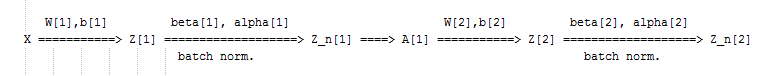
\includegraphics[width=1.0\textwidth]{img/c2/bn.png}
    \caption{Workflow of 2 layers NN with batch normalization.}
    \label{fig:my_label}
\end{figure}

$\beta[i]$ and $\gamma[i]$ are updated using any optimization algorithms (like GD, Momentum, RMSprop, Adam).

Batch normalization is usually applied with mini-batches.

Shapes: $Z[l] - (n[l], m), \beta[l] - (n[l], m), \gamma[l] - (n[l], m)$.

\subsubsection{Why Does Batch Normalization Work?}
The first reason is the same reason as why we normalize X (Shape the inputs and makes loss reach minimum point faster).

The second reason is that batch normalization reduces the problem of input values changing (shifting).

\subsubsection{Batch Normalization at Test Time}
When we train a NN with batch normalization, we compute the mean and the variance of the mini-batch.

In testing we might need to process examples one at a time. The mean and the variance of one example won't make sense. We have to compute an estimated value of mean and variance to use it in testing time.

We can use the weighted average cross the mini-batches. We will use the estimated values of the mean and variance to test. This method is also sometimes called "running average".

In practice most often you will use a deep learning framework and it will contain some default implementation of doing such a thing.

\subsubsection{Softmax Regression}
In every example we have used so far we were talking about binary classification. There are a generalization of logistic regression called softmax regression that is used for multiclass classification/regression.

Each of C values in the output layer will contain a probability of the example to belong to each of the classes. In the last layer we will have to activate the softmax activation function instead of the sigmoid activation.

\begin{equation}
    A[L] = \frac{e^{z[L]}}{\sum e^{z[L]}}
\end{equation}

\subsubsection{Training a Softmax Classifier}
There is an activation which is called hard max, which gets 1 for the maximum value and zeros for the others. If you are using NumPy, it's np.max over the vertical axis.

The softmax name came from softening the values and not harding them like hard max.

Softmax is a generalization of logistic activation function to C classes. If C = 2 softmax reduces to logistic regression.

The loss function used with softmax:

\begin{equation}
    L (y, \hat{y}) = - \sum y_j * \log \hat{y}_j,\ \ j: 0\to C-1
\end{equation}

With m examples:

\begin{equation}
    L (Y, \hat{Y}) = - \frac{1}{m} \sum y_j^{(i)} * \log \hat{y}_j^{(i)},\ \ j: 0\to C-1, i: 0\to m
\end{equation}

Back propagation with softmax:

\begin{equation}
    dZ[L] = \hat{Y} - Y
\end{equation}

That's all for Course II: Improving Deep Neural Networks: Hyperparameter tuning, Regularization and Optimization.

\newpage


\section{Structuring Machine Learning Projects}
This is the third course of deep learning specialization at Coursera taught by Professor Andrew Ng. Here is my certificate after finishing this course (Fig. \ref{C3-Certificate}):

\begin{figure}[!htbp]
    \centering
    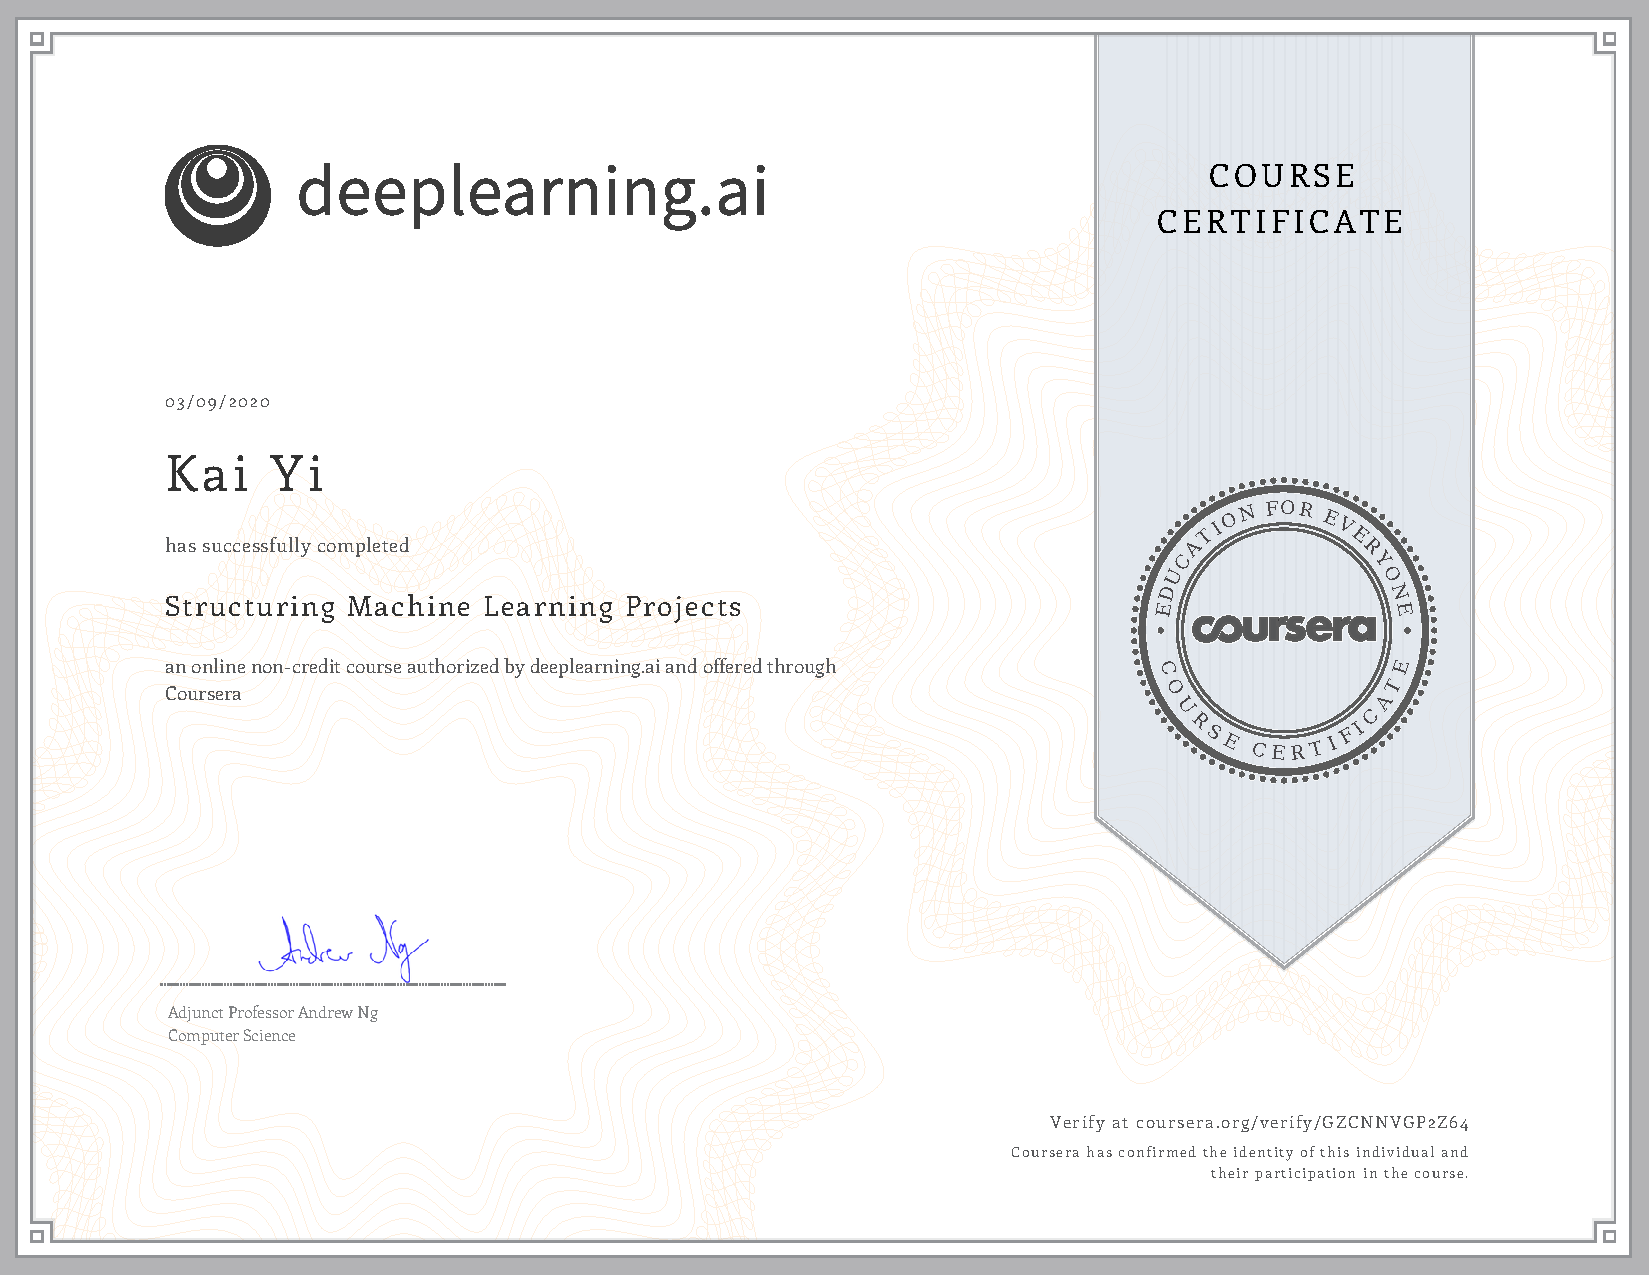
\includegraphics[width=1.0\textwidth]{img/C3-Certificate.pdf}
    \caption{Certificate of Structuring Machine Learning Projects. Obtained in Mar. 2020.}
    \label{C3-Certificate}
\end{figure}

\subsection{Course Overview}
According to the official site of this course, there are following key components:

\begin{itemize}
    \item Understand how to diagnose errors in a machine learning system.
    \item Be able to prioritize the most promising directions for reducing error.
    \item Understand complex ML settings, such as mismatched training sets, and comparing to and/or surpassing human-level performance.
    \item Know how to apply end-to-end learning, transfer learning, and multi-task learning.
\end{itemize}

\subsection{Machine Learning (ML) Strategy I}
\subsubsection{Why ML Strategy}
You have a lot of ideas for how to improve the accuracy of your deep learning system:

\begin{itemize}
    \item Collect more data.
    \item Collect more diverse training set.
    \item Train algorithm longer with gradient descent.
    \item Try different optimization algorithm (e.g. Adam)
    \item Try bigger network.
    \item Try smaller network.
    \item Try dropout.
    \item Add L2 regularization.
    \item Change network architecture (activation functions, nums of hidden units, etc)
\end{itemize}

This course will give you some strategies to help analyze your problem to go in a direction that will help you get better results.

\subsubsection{Orthogonalization}
Some deep learning developers know exactly what hyperparameter to tune in order to try to achieve one effect. This is a process we call orthogonalization.

In orthogonalization, you have some controls, but each control does a specific task and doesn't affect other controls.

For a supervised learning system to do well, you usually need to tune the knobs of your system to make sure that four things hold true -chain of assumptions in machine learning:

\begin{itemize}
    \item You'll have to fit training set well on cost function (near human level performance if possible). (If it's not achieved you could try bigger network, another optimization algorithm (like Adam)...)
    \item Fit dev set well on cost function. (If it's not achieved you could try regularization, bigger training set...)
    \item Fit test set well on cost function. (If it's not achieved you could try bigger dev set...)
    \item Performs well in real world. (If it's not achieved you could try to change dev set, change cost function...)
\end{itemize}

\subsubsection{Single Number Evaluation Metric}
It's better and faster to set a single number evaluation metric for your project before you start it.

Difference between precision and recall (in cat classification example):

\begin{itemize}
    \item Suppose we run the classifier on 10 images which are 5 cats and 5 non-cats. The classifier identifies that there are 4 cats, but it identified 1 wrong cat.
    \item Confusion matrix (Table \ref{confusion-matrix}).
\end{itemize}

\begin{table}[!htbp]
    \centering
    \begin{tabular}{c|c|c}
        \hline
        - & Predicted Cat & Predicted Non-Cat \\
        \hline
        Actual Cat & 3 & 2\\
        Actual Non-Cat & 1 & 4\\
        \hline
    \end{tabular}
    \caption{Confusion matrix.}
    \label{confusion-matrix}
\end{table}

\begin{itemize}
    \item Precision: percentage of true cats in the recognized result: P = 3/(3+1)
    \item Recall: percentage of true recognition cat of the all cat predictions: R = 3/(3+2)
    \item Accuracy: (3+4)/10
\end{itemize}

Using a precision/recall for evaluation is good in a lot of cases, but separately they don't tell you which algorithm is better. E.g. (Table \ref{pr-classifiers}):

\begin{table}[!htbp]
    \centering
    \begin{tabular}{c|c|c}
        \hline
        Classifier & Precision & Recall \\
        \hline
        A & 95\% & 90\%\\
        B & 98\% & 85\%\\
        \hline
    \end{tabular}
    \caption{Precision and recall of two classifiers.}
    \label{pr-classifiers}
\end{table}

A better thing is to combine precision and recall in one single (real) number evaluation metric. There is a metric called F1 score, which combines them:

\begin{itemize}
    \item You can think of F1 score as an average of precision and recall (Equation \ref{f1-matrix}).
\end{itemize}

\begin{equation}\label{f1-matrix}
    F1 = \frac{2}{\frac{1}{P} + \frac{1}{R}}
\end{equation}

\subsubsection{Satisfying and Optimizing Metric}
Its hard sometimes to get a single number evaluation metric. E.g. (Table \ref{pr-mixclassify}):

\begin{table}[!htbp]
    \centering
    \begin{tabular}{c|c|c}
        \hline
        Classifier & F1 & Running Time \\
        \hline
        A & 90\% & 80 ms\\
        B & 92\% & 95 ms\\
        C & 92\% & 1,500 ms\\
        \hline
    \end{tabular}
    \caption{F1 and Running Time of 3 classifiers.}
    \label{pr-mixclassify}
\end{table}

So we can solve that by choosing a single optimizing metric and decide that other metrics are satisfying. E.g.:

\begin{itemize}
    \item Maximize 1 (F1 here) \ \ \# optimizing metric (one optimizing metric)
    \item subject to N-1 satisfying metrics (running time < 1, 000 here)\ \ \# (N-1 satisfying metrics)
\end{itemize}

\subsubsection{Train/dev/test Distributions}
Dev and test sets have to come from the same distribution.

Choose dev set and test set to reflect data that you expect to get in the future and consider important to do well on.

Setting up the dev set, as well as the validation metric is really defining what target you want to aim at.

\subsubsection{Size of the Dev and Test Sets}
An old way of splitting the data was 70\% training, 30\% test or 60\% training, 20\% dev and 20\% test.

The old way was valid for a number of examples ~<100000.

In the modern deep learning if you have a million or more examples a reasonable split wound be 98\% training, 1\% dev and 1\% test.

\subsubsection{When to Change Dev/Test Sets and Metrics}
Let's take an example. In a cat classification example we have these matric results (Table \ref{when2change}):

\begin{table}[!htbp]
    \centering
    \begin{tabular}{c|c}
        \hline
        Algorithm &  Classification Error\\
        \hline
        A & 3\% error (but a lot of porn images are treated as cat images here)\\
        B & 5\% error\\
        \hline
    \end{tabular}
    \caption{Example of "When to Change Dev/Test Sets and Metrics".}
    \label{when2change}
\end{table}

In the above example if we choose the best algorithm by metric it would be "A", but if the users decide if will be "B".

Thus in this case, we want and need to change our metric. The solution is to add weights to select from different criterion.

Conclusion: If doing well on your metric + dev/test set doesn't correspond to doing well in your application, change your metric and/or dev/test set.

\subsubsection{Why human-level performance?}
We compare to human-level performance because of two main reasons:
\begin{itemize}
    \item Because of advances in deep learning, machine learning algorithms are suddenly working much better and so it has become much more feasible in a lot of application areas for machine learning algorithms to actually become competitive with human-level performance.
    \item It turns out that the workflow of designing and building a machine learning system is much mor efficient when you're trying to don something that humans can also do.
\end{itemize}

After an algorithm reaches the human level performance the progress of accuracy slow don \ref{humanlevelperformance}.

\begin{figure}
    \centering
    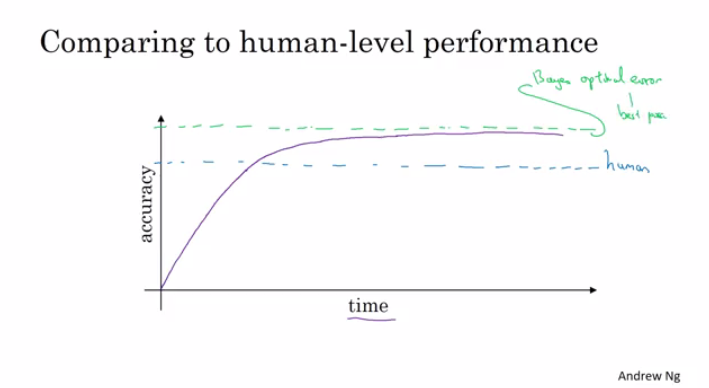
\includegraphics[width=1.0\textwidth, trim={20 50 0 50}, clip]{img/c2/human-level_performance.png}
    \caption{Comparing to human level performance.}
    \label{humanlevelperformance}
\end{figure}

You won't surpass an error that's called "Bayes optimal error".

There isn't much error range between human-level error and Bayes optimal error in computer vision tasks.

Humans are quite good at a lot of tasks. So as long as the machine learning method is worse than humans, you can:

\begin{itemize}
    \item Get labeled data from humans.
    \item Gain insight from manual error analysis: why did a person get it right?
    \item Better analysis of bias/variance.
\end{itemize}

\subsubsection{Avoidable Bias}
Suppose that the cat classification algorithm gives these results (Table \ref{avoidable-bias}):

\begin{table}[!htbp]
    \centering
    \begin{tabular}{c|c|c}
        \hline
        Humans & 1\% & 7.5\% \\
        Training Error & 8\% & 8\%\\ 
        Dev Error & 10\% & 10\%\\
        \hline
    \end{tabular}
    \caption{Example of avoidable bias.}
    \label{avoidable-bias}
\end{table}

In the left example, because the human level error is 1\% then we have to focus on the bias.

In the right example, because the human level error is 7.5\% then we have to focus on the variance.

The human-level error as a proxy (estimate) for Bayes optimal error. Bayes optimal error is always less (better), but human-level in most cases is not far from it.

Avoidable bias = Training error - Human (Bayes) error

Variance = Dev error - Training error

\subsubsection{Understanding Human-Level Performance}
When choosing human-level performance, it has to be chosen in the terms of what you want to achieve with the system.

You might have multiple human-level performances based on the human experience. Then you choose the human-level performance (proxy for Bayes error) that is more suitable for the system you're trying to build.

Improving deep learning algorithms is harder once you reach a human-level performance.

Summary of bias/variance with human-level performance:

\begin{itemize}
    \item Human-level error (proxy for Bayes error). Calculate avoidable bias = training error - human-level error. If avoidable bias difference is the bigger, then it's bias problem and you should use a strategy for bias resolving.
    \item Training error. Calculate variance = dev error - training error. If variance difference is bigger, then you should use a strategy for variance resolving.
    \item Dev error.
\end{itemize}

So having an estimate of human-level performance gives you an estimate of Bayes error. And this allows you to more quickly make decisions as to whether you should focus on trying to reduce a bias or trying to reduce the variance of your algorithm.

These techniques will tend to work well until you surpass human-level performance, whereupon you might no longer have a good estimate of Bayes error that still helps you make this decision really clearly.

\subsubsection{Surpassing Human-Level Performance}
In some problems, deep learning has surpassed human-level performance. Like:

\begin{itemize}
    \item Online advertising
    \item Product recommendation
    \item Load approval
\end{itemize}

The listed examples are not natural perception task. Humans are far better in natural perception tasks like computer vision and speech recognition. It's harder for machines to surpass human-level performance in natural perception task. But there are already some systems that achieved it.

\subsubsection{Improving Your Model Performance}
To improve your deep learning supervised system follow these guidelines:

\begin{itemize}
    \item[i.] Look at the difference between human level error and the training error - avoidable bias.
    \item[ii.] Look at the difference between the dev/test set and training set error - variance.
    \item[iii.] If avoidable bias is large you have these options: 1) Train bigger model; 2) Train longer/better optimization algorithm (like Momentum, RMSprop, Adam); 3) Find better NN architecture/hyperparameters search.
    \item[iv.] If variance is large you have these options: 1) Get more training data; 2) Regularization (L2, dropout, data augmentation); 3) Find better NN architecture/hyperparameters search.
\end{itemize}

\subsection{Machine Learning Strategy II}
\subsubsection{Carrying Out Error Analysis}
Error analysis - process of manually examining mistakes that your algorithm is making. It can give you insights into what to do next. E.g.:

\begin{itemize}
    \item In the cat classification example, if you have 10\% error on your dev set and you want to decrease the error.
    \item You discovered that some of the mislabeled data are dog pictures that look like cats. Should you try to make your cat classifier do better on dogs (this could take some weeks)?
    \item Error analysis approach:
    \begin{itemize}
        \item Get 100 mislabeled dev set examples at random.
        \item Count up how many are dogs.
        \item If 5 of 100 are dogs then training your classifier to do better on dogs will decrease your error up to 9.5\% (called ceiling), which can be too little.
        \item If 50 of 100 are dogs then you could decrease your error up to 5\%, which is reasonable and you should work on that.
    \end{itemize}
\end{itemize}

Based on the above example, error analysis helps you to analyze the error before taking an action that could take a lot of time with no need.

Sometimes, you can evaluate multiple error analysis ideas in parallel and choose the best idea. Create a spreadsheet to do that and decide, e.g. (Table \ref{error-analysis}):

\begin{table}[!htbp]
    \centering
    \begin{tabular}{c|c|c|c|c|c}
        \hline
        Image & Dog & Great Cats & Blurry & Instagram Filters & Comments \\
        \hline
        1 & $\surd$ & & & $\surd$ & Pitbull\\
        2 & $\surd$ & & $\surd$ & $\surd$ &\\
        3 &&&&& Rainy day at zoo\\
        4 && $\surd$&&&\\
        $\cdots$ &&&&&\\
        \hline
        \% totals & 8\% & 43\% & 61\% & 12\% & \\
        \hline
    \end{tabular}
    \caption{Spreadsheet of 100 selected images for error analysis.}
    \label{error-analysis}
\end{table}

In the above example you will decide to work on great cats or blurry images to improve your performance.

This quick counting procedure, which you can often do in, at most, small numbers of hours can really help you make much better prioritization decisions, and understand how promising different approaches are to work on.

\subsubsection{Cleaning Up Incorrectly Labeled Data}
Deep learning algorithms are quite robust to random errors in the training set but less robust to systematic errors. But it's OK to go and fix these labels if you can.

If you want to check for mislabeled data in dev/test set, you should also try error analysis with the mislabeled column. E.g. (Table \ref{mislabeled}):

\begin{table}[!htbp]
    \centering
    \begin{tabular}{c|c|c|c|c|c}
        \hline
        Image & Dog & Great Cats & Blurry & Mislabeled & Comments \\
        \hline
        1 & $\surd$ & & & $\surd$ & Pitbull\\
        2 & $\surd$ & & $\surd$ & $\surd$ &\\
        3 &&&&& Rainy day at zoo\\
        4 && $\surd$&&&\\
        $\cdots$ &&&&&\\
        \hline
        \% totals & 8\% & 43\% & 61\% & 12\% & \\
        \hline
    \end{tabular}
    \caption{Spreadsheet of 100 selected images for error analysis.}
    \label{mislabeled}
\end{table}

Then: If overall dev set error is 10\%, then errors due to incorrect data is 0.6\% while the errors due to other causes is 9.0\%. Thus you should focus on the 9.4\% error rather than the incorrect data.

Consider these guidelines while correcting the dev/test mislabeled examples:

\begin{itemize}
    \item Apply the same process to your dev and test sets to make sure they continue to come from the same distribution.
    \item Consider examining examples your algorithm got right as well as ones it got wrong. (Not always done if you reached a good accuracy)
    \item Train and (dev/test) data may now come from a slightly different distributions.
    \item It's very important to have dev and test sets to come from the same distribution. But it could be OK for a train set to come from slightly different distribution.
\end{itemize}

\subsubsection{Build You First System Quickly, Then Iterate}
The steps you take to make your deep learning project:

\begin{itemize}
    \item Setup dev/test set and metric.
    \item Build initial system quickly.
    \item Use bias/variance analysis \& error analysis to prioritize next steps.
\end{itemize}

\subsubsection{Training and Testing on Different Distributions}
A lot of teams are working with deep learning applications that have training sets that are different from the dev/test sets due to the hunger of deep learning to data.

There are some strategies to follow up when training set distribution differs from dev/test sets distribution:

\begin{itemize}
    \item Option I (not recommended): shuffle all the data together and extract randomly training and dev/test sets.
    \begin{itemize}
        \item Advantages: all the sets now come from the same distribution.
        \item Disadvantages: the other (real world) distribution that was in the dev/test sets will occur less in the new dev/test sets and that might be not what you want to achieve.
    \end{itemize}
    \item Option II: take some of the dev/test set examples and add them to the training set.
    \begin{itemize}
        \item Advantages: the distribution you care about is the target now.
        \item Disadvantages: the distributions in training and dev/test sets are now different. But you will get a better performance over a long time.
    \end{itemize}
\end{itemize}

\subsubsection{Bias and Variance With Mismatched Data Distributions}
Bias and variance analysis changes when training and dev/test set is from the different distribution.

Example: the cat classification example. Suppose you've worked in the example and reached this:

\begin{itemize}
    \item Human error: 0\%
    \item Train error: 1\%
    \item Dev error: 10\%
\end{itemize}

In this example, you may think this is a variance problem, but because the distributions aren't the same you can't tell for sure. Because it could be that train set was easy to train on, but the dev set was more difficult.

To solve this issue, we create a new set called train-dev set as a random subset of the training set (so it has the same distribution) and we get:

\begin{itemize}
    \item Human error: 0\%
    \item Train error: 1\%
    \item Train-dev error: 9\%
    \item Dev error: 10\%
\end{itemize}

Now we are sure that this is a high variance problem.

Suppose we have a different situation:

\begin{itemize}
    \item Human error: 0\%
    \item Train error: 1\%
    \item Train-dev error: 1.5\%
    \item Dev error: 10\%
\end{itemize}

In this case, we have something called \textit{data mismatch} problem.

Conclusions:

\begin{itemize}
    \item Human-level error (proxy for Bayes error)
    \item Train error
    \begin{itemize}
        \item Calculate \textit{avoidable bias = training error - human level error}.
        \item If the difference is big then its Avoidable bias problem then you should use a strategy for high bias.
    \end{itemize}
    \item Train-dev error
    \begin{itemize}
        \item Calculate \textit{variance = training-dev error - training error}.
        \item If the difference is big then its high variance problem then you should use a strategy for solving it.
    \end{itemize}
    \item Dev error
    \begin{itemize}
        \item Calculate \textit{data mismatch = dev error - train-dev error}.
        \item If difference is much bigger then train-dev error its Data mismatch problem.
    \end{itemize}
    \item Test error
    \begin{itemize}
        \item Calculate \textit{degree of overfitting to dev set = test error - dev error}.
        \item Is the difference is big (positive) then maybe you need to find a bigger dev set (dev set and test set come from the same distribution, so the only way for there to be a huge gap here, for it to do much better on the dev set than the test set, is if you somehow managed to overfit the dev set).
    \end{itemize}
\end{itemize}

Unfortunately, there aren't many systematic ways to deal with data mismatch. There are some things to try about this in the next section.

\subsubsection{Addressing Data Mismatch}
There aren't completely systematic solutions to this, but there are some things you could try.

\begin{itemize}
    \item Carry out manual error analysis to try to understand the difference between training and dev/test sets.
    \item Make training data more similar, or collect more data similar to dev/test sets.
\end{itemize}

If your goal is to make the training data more similar to your dev set one of the techniques you can use is \textit{artificial data synthesis} that can help you make more training data.

\begin{itemize}
    \item Combine some of your training data with something that can convert it to the dev/test set distribution. E.g.:
    \begin{itemize}
        \item Combine normal audio with car noise to get audio with car noise example.
        \item Generate cars using 3D graphics in a car classification example.
    \end{itemize}
    \item Be cautious and bear in mind whether or not you might be accidentally simulating data only from a tiny subset of the space of all possible examples because your NN might overfit these generated data (like particular car noise or a particular design of 3D graphics cars).
\end{itemize}

\subsubsection{Transfer Learning}
Apply the knowledge you took in a task A and apply it in another task B.

For example, you have trained a cat classifier with a lot of data, you can use the part of the trained NN to solve medical image classification problem.

To do transfer learning, delete the last few layers of NN and theis weights and:

\begin{itemize}
    \item Option I: If you have a small data set - keep all the other weights as a fixed weights. Add a new last layer(-s) and initialize the new layer weights and feed the new data to the NN and learn the new weights.
    \item Option II: If you have enough data you can retrain all the weights.
\end{itemize}

Option I and II are called \textbf{fine-tuning} and training on task A called \textbf{pretraining}.

When transfer learning make sense:

\begin{itemize}
    \item Task A and B have the same input X (e.g. image, audio).
    \item You have a lot of data for the task A you are transferring from and relatively less data for the task B your transferring to.
    \item Low level features from task A could be helpful for learning task B.
\end{itemize}

\subsubsection{Multi-Task Learning}
Whereas in transfer learning, you have a sequential process where you learn from task A and then transfer that to task B. In multi-task learning, you start off simultaneously, trying to have one neural network do several things at the same time. And then each of these tasks helps hopefully all of the other tasks.

Example: You want to build an object recognition system that detects pedestrians, cars, stop signs and traffic lights (image has multiple labels).

Then Y shape will be (4,m) because we have 4 classes and each one is a binary one.

Then.

\begin{equation}
\begin{aligned}
    Cost &= \frac{1}{m} \sum^m_{i=1}\sum_{j=1}^{4} L(\hat{y}^{i}_j, y^{i}_j), \ \ i = 1\to m, j = 1\to 4\\
    L &= - y^i_j * \log (\hat{y}^i_j) - (1 - y^i_j) * \log (1 - \hat{y}^i_j)\\
\end{aligned}
\end{equation}

In the above example, you could have trained 4 neural networks separately but if some of the earlier features in NN can be shared among these different types of objects, then you find that training one NN to do four things results in better performance than training 4 completely separate NNs to do the four tasks separately.

Multi-task learning will also work if y isn't complete for some labels. E.g.:

\begin{lstlisting}
Y = [1 ? 1 ...]
    [0 0 1 ...]
    [? 1 ? ...]
\end{lstlisting}

In the above case, it will do good with the missing data, just the loss function will be different:

\begin{equation}
    \begin{aligned}
        L &= - y^i_j * \log (\hat{y}^i_j) - (1 - y^i_j) * \log (1 - \hat{y}^i_j)\ \  for\  all \ j \ which \  y^i_j != ?\\
    \end{aligned}
\end{equation}

Multi-task learning makes sense:

\begin{itemize}
    \item Training on a set of tasks that could benefit from having shared lower-level features.
    \item Usually, amount of data you have for each task is quite similar.
    \item Can train a big enough network to do well on all the tasks.
\end{itemize}

If you can train a big enough NN, the performance of the multi-task learning compared to splitting the tasks is better.

Today transfer learning is used more often than multi-task learning. But in the area of computer vision, multi-task learning is widely adapted.

\subsubsection{What Is End-to-end Deep Learning}
Some systems have multiple stages to implement. An end-to-end deep learning system implements all these stages with a single NN. E.g.:

\begin{itemize}
    \item Speech recognition system:
\begin{lstlisting}[language=python]
# non-end-to-end system
Audio ---> Features --> Phonemes --> Words --> Transcript    
# end-to-end deep learning system
Audio ---------------------------------------> Transcript    
\end{lstlisting}
    \item End-to-end deep learning gives data more freedom, it might not use phonemes when traning.
\end{itemize}

To build the end-to-end deep learning system that works well, we need a big dataset (more data then in non end-to-end system). If we have a small dataset the ordinary implementation could work just fine.

Another example of end-to-end learning:

\begin{itemize}
    \item Face recognition system:
\begin{lstlisting}[language=python]
# end-to-end deep learning system
Image ---------------------> Face recognition
# deep learning system - best approach for now
Image --> Face detection --> Face recognition    
\end{lstlisting}
    \item In practice, the best approach is the second one for now.
    \item In the second implementation, it's a two steps approach where both parts are implemented using deep learning.
    \item Its working well because it's harder to get a lot of pictures with people in front of the camera than getting faces of people and compare them.
    \item In the second implementation at the last step, the NN takes two faces as an input and outputs if the two faces are the same person or not (Siamese Neural Network\cite{koch2015siamese}).
\end{itemize}

Example 3:

\begin{itemize}
    \item Machine translation system:
\begin{lstlisting}[language=python]
# non-end-to-end system
English --> Text analysis --> ... --> French    
# end-to-end deep learning system - best approach
English ----------------------------> French    
\end{lstlisting}
    \item Here end-to-end deep leaning system works better because we have enough data to build it.
\end{itemize}

Example 4:

\begin{itemize}
    \item Estimating child's age from the x-ray picture of a hand:
\begin{lstlisting}[language=python]
# non-end-to-end system - best approach for now
Image --> Bones --> Age   
# end-to-end deep learning system
Image ------------> Age    
\end{lstlisting}
    \item In this example non-end-to-end system works better because we don't have enough data to train end-to-end system.
\end{itemize}

\subsubsection{Whether to Use End-to-end Deep Learning}
Pros of end-to-end deep learning:
\begin{itemize}
    \item Let the data speak. By having a pure machine learning approach, your NN learning input from X to Y may be more able to capture whatever statistics are in the data, rather than being forced to reflect human preconceptions.
    \item Less hand-designing of components needed.
\end{itemize}

Cons of end-to-end deep learning:
\begin{itemize}
    \item May need a large amount of data.
    \item Excludes potentially useful hand-design components (it helps more on the smaller dataset).
\end{itemize}

Applying end-to-end deep learning:
\begin{itemize}
    \item Key question: Do you have sufficient data to learn a function of the \textbf{complexity} needed to map x to y?
    \item When applying supervised learning you should carefully choose what types of X to Y mappings you want to learn depending on what task you can get data for.
\end{itemize}
\newpage
\section{Convolutional Neural Networks}  
This is the fourth course of deep learning specialization at Coursera taught by Professor Andrew Ng. Here is my certificate after finishing this course (Fig. \ref{C4-Certificate}):

\begin{figure}[!htbp]
    \centering
    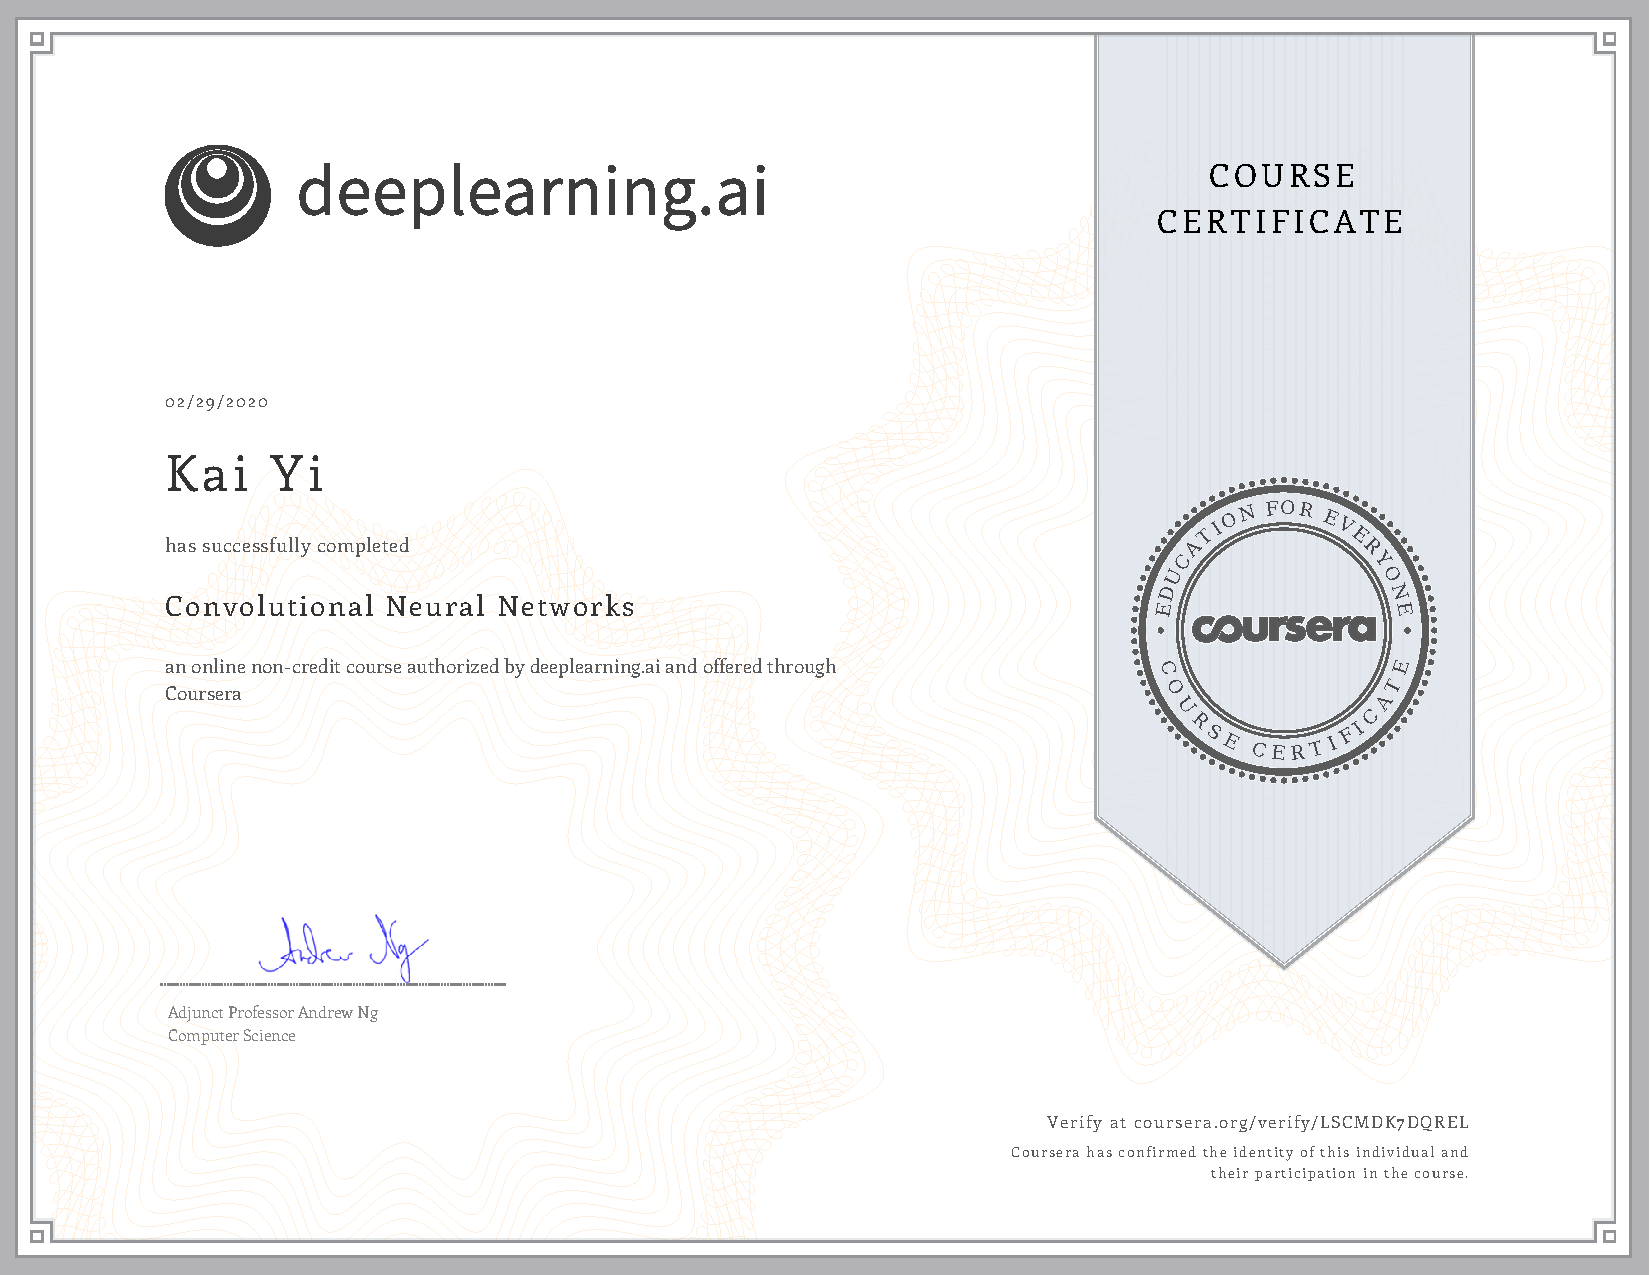
\includegraphics[width=1.0\textwidth]{img/C4-Certificate.pdf}
    \caption{Certificate of Convolutional Neural Networks. Obtained in Feb. 2020.}
    \label{C4-Certificate}
\end{figure}

\subsection{Course Overview}
According to the official site of this course, there are following key components:

\begin{itemize}
    \item Understand how to build a convolutional neural network, including recent variations such as residual networks.
    \item Know how to apply convolutional networks to visual detection and recognition tasks.
    \item Know to use neural style transfer to generate art.
    \item Be able to apply these algorithms to a variety of image, video, and other 2D or 3D data.
\end{itemize}

\subsection{Foundations of CNNs}
The aims of this section is to implement the foundational layers of CNNs (pooling, convolutions) and to stack them properly in a deep network to solve multi-class image classification problems.

\subsubsection{Edge Detection Example}
Early layers of CNN might detect edges then the middle layers will detect parts of objects and the later layers will put these parts together to produce an output.

\subsubsection{Padding, Stride}
\begin{equation}
    C_{out} = (C_{in} - k + 2*p) / s + 1
\end{equation}

k represents the kernel size, p represents padding and s represents stride.

\subsubsection{Pooling layers}
Other than the conv layers, CNNs often uses pooling layers to reduce the size of the inputs, speed up computation, and to make some of the features it detects more robust.

The max pooling is saying, if the feature is detected anywhere in this filter then keep a high number. But the main reason why people are using pooling because its works well in practice and reduce computations.

Max pooling has no parameters to learn.

Average pooling is taking the averages of the values instead of taking the max values.

Max pooling is used more often than average pooling in practice.

If stride of pooling equals the size, it will then apply the effect of shrinking.

\subsubsection{Convolutional Neural Network Example}
Here are some statistics about a mentioned example (Fig. \ref{cnn-example}):

\begin{figure}[!htbp]
    \centering
    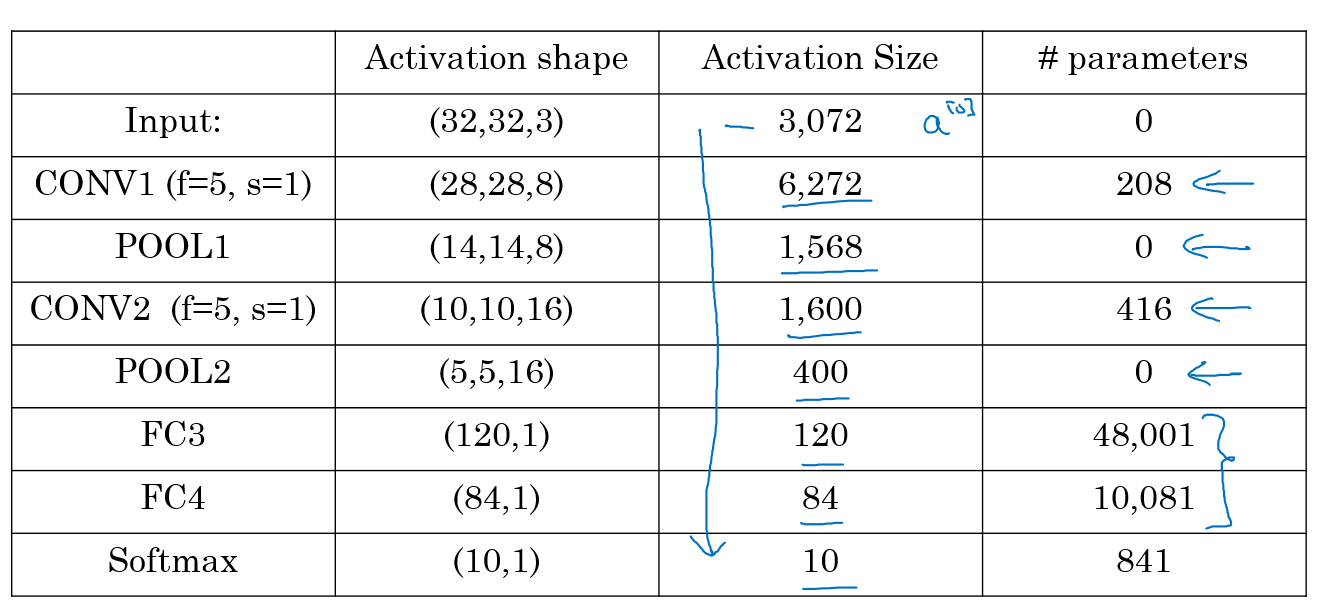
\includegraphics[width=1.0\textwidth]{img/c4/cnn-examples.png}
    \caption{Some statistics about a LeNet-like network. Every parameter is calculated by $(k^2+1)*c$, k represents kernel size and c represents output channel.}
    \label{cnn-example}
\end{figure}

Usually the input size decreases over layers which the number of filters increases.

A CNN usually consists of one or more convolution (not just one as the shown example) followed by a pooling.

Fully connected layers has the most parameters in the network.

\subsubsection{Why Convolutions?}
Two main advantages of Convs are:

\begin{itemize}
    \item Parameter sharing. A feature detector (such as a vertical edge detector) that's useful in one part of the image is probably useful in another part of the image.
    \item Sparsity of Connections. In each layer, each output value depends only on a small number of inputs which makes it translation invariance (Translation invariance means that the system produces exactly the same response, regardless of how its input is shifted.).
\end{itemize}

\subsection{Deep Convolutional Models: Case Studies}
The goal of this section is to learn about the practical tricks and methods used in deep CNNs straight from the research papers.

\subsubsection{Classic Networks}
In this subsection we will talk about classic networks which are LeNet-5, AlexNet and VGG.

\paragraph{LeNet-5} The goal for this model was to identify handwritten digits in a $32\times 32\times 1$ gray image. Here is the drawing of it (Fig. \ref{lenet}):

\begin{figure}[!htbp]
    \centering
    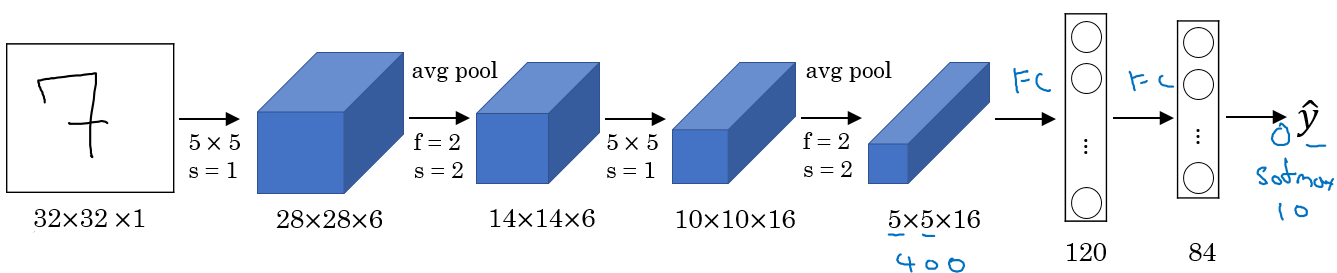
\includegraphics[width=1.0\textwidth]{img/c4/lenet.png}
    \caption{LeNet architecture.}
    \label{lenet}
\end{figure}

This model was published in 1998 \cite{lecun1998gradient}. The last layer wasn't using softmax back then.

It has 60k parameters.

The dimensions of the image decreases as the number of channels increases.

$Conv \to Pool \to Conv \to Pool \to FC \to FC \to Softmax$ this type of arrangement is quite common.

The activation function used in the paper was Sigmoid and Tanh. Modern implementation uses ReLU in most of the cases.

\paragraph{AlexNet} Named after Alex Krizhevsky who was the first author of this paper \cite{krizhevsky2012imagenet}. The other authors includes Geoffrey Hinton.

The goal for this model was the ImageNet challenge which classifies images into 1000 classes. Here are the drawing of this model:

\begin{figure}[!htbp]
    \centering
    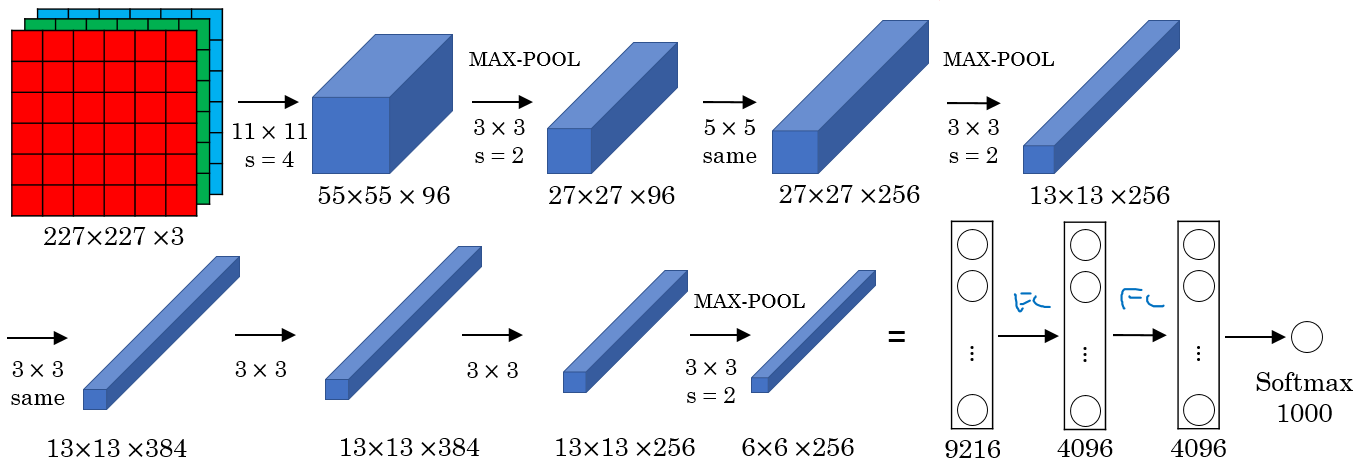
\includegraphics[width=1.0\textwidth]{img/c4/alexnet.png}
    \caption{AlexNet architecture.}
    \label{lenet}
\end{figure}

Architecture:

$Conv \to Max-pool\to Conv\to Max-pool\to Conv\to Conv\to Conv\to Max-pool\to Flatten\to FC\to FC\to Softmax$

Similar to LeNet-5 but bigger.

Has 60 million parameters compared to 60k parameterof LeNet-5.

It used the ReLU activation function.

The original paper contains multiple GPUs and Local Response Normalization (LRN). Multiply GPUs were used because the GPUs were not so fast back then. Researchers proved that LRN doesn't help much so for now don't botter yourself for understanding or implementing it.

This paper convinced the computer vision researchers that deep learning is so important.

\paragraph{VGG-16} VGG-16 \cite{simonyan2014very} is a modification fro AlexNet.

Instead of having a lot of hyperparameters let's have some simpler network.

Focus on having only these blocks:
\begin{itemize}
    \item Conv = $3\times 3$, filter, s = 1, 'SAME'
    \item Max-Pool = $2\times 2$, s = 2
\end{itemize}

Here is the architecture (Fig. \ref{vgg16}):

\begin{figure}[!htbp]
    \centering
    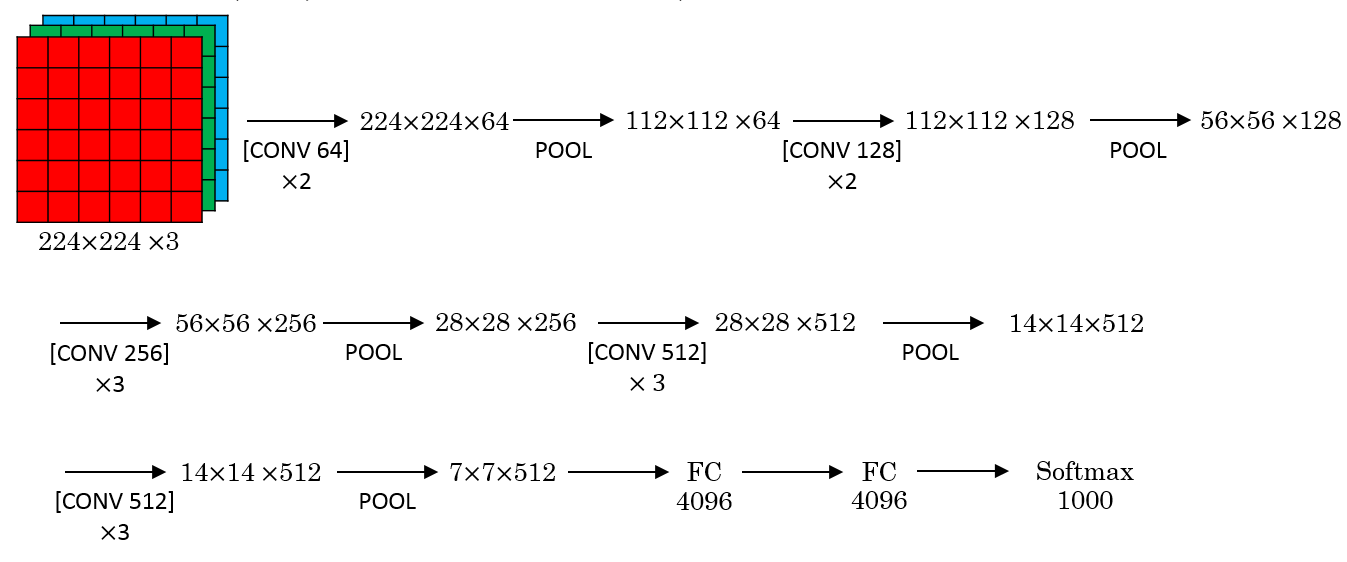
\includegraphics[width=1.0\textwidth]{img/c4/vgg16.png}
    \caption{VGG-16 architecture.}
    \label{vgg16}
\end{figure}

This network is large even by modern standards. It has around 138 million parameters (Most of the parameters are in the fully connected layers).

In has a total memory of 96MB per image for only forward propagation (Most memory are in the earlier layers).

Number of filers increases from 64 to 128 to 256 to 512. 512 was made twice.

Pooling was the only one who is responsible for shrinking the dimensions.

There are another version called VGG-19 which is a bigger version. But most people uses the VGG-16 instead of the VGG-19 because it does the same.

VGG paper is attractive it tries to make some rules regarding using CNNs.

\subsubsection{Residual Networks (ResNets)}
Very, very deep NNs are difficult to train becaus of vanishing and exploding gradiednts problems.

In this section we will learn about skip connection which makes you take the activation from one layer and subsequently feed it to another layer even much deeper in NN which allows you to train large NNs even with layers greater than 100.

\paragraph{Residual Block}
ResNets are built out of some Residual blocks (Fig. \ref{resblock}).

\begin{figure}[!htbp]
    \centering
    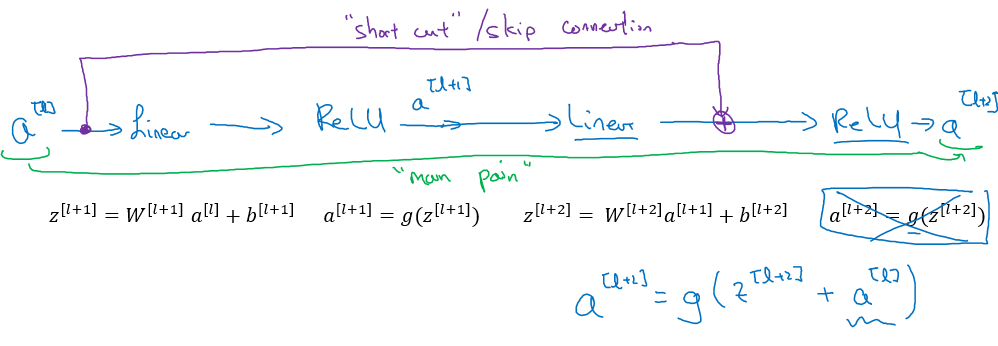
\includegraphics[width=1.0\textwidth]{img/c4/resblock.png}
    \caption{Residual block architecture.}
    \label{resblock}
\end{figure}

They add a shortcut/skip connection before the second activation.

The authors of this block find that you can train a deeper NNs by stacking this block.

\paragraph{Residual Network}
Are a NN that consists of some Residual blocks (Fig. \ref{resnet}).

\begin{figure}[!htbp]
    \centering
    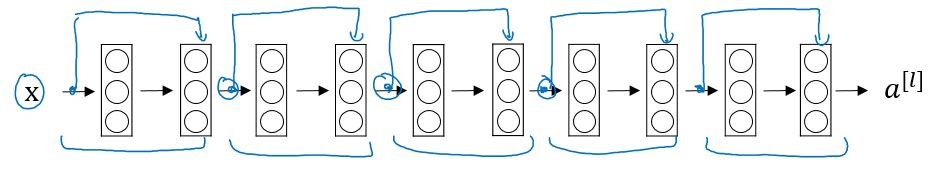
\includegraphics[width=1.0\textwidth]{img/c4/resnet.png}
    \caption{Residual network architecture.}
    \label{resnet}
\end{figure}

These networks can go deeper without hurting the performance. In the normal NN - Plain networks - the theory tell us that if we go deeper we will get a better solution to out problem, but because of the vanishing and exploding gradients problems the performances of the network suffers as it goes deeper. Thanks to Residual Network we can go deeper as we want now (Fig. \ref{plain-vs-resnet}).

\begin{figure}[!htbp]
    \centering
    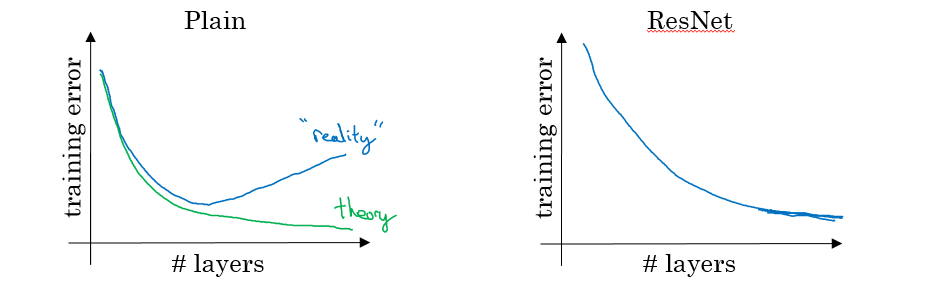
\includegraphics[width=1.0\textwidth]{img/c4/plain-vs-resnet.png}
    \caption{Plain networks vs. ResNet}
    \label{plain-vs-resnet}
\end{figure}

On the left is the normal NN and on the right are the ResNet. As you can see the performance of ResNet increases as the network goes deeper.

In some cases going deeper won't effect the performance and that depends on the problem on your hand.

Some people are trying to train 1000 layer now which isn't used in practice.

\subsubsection{Why ResNets Work}
Lets see some example that illustrates why ResNets work.

We have a big NN as the following: $X \to Big\ NN\to a[l]$.

Lets add two layers to this network as a residual block: $X \to Big\ NN\to a[l] \to layer1 \to layer2\to a[i+2]$. $a[i]$ has a direct connection to $a[i+2]$.

Suppose we are using ReLU activations.

Then:

\begin{lstlisting}
a[l+2] = g(z[l+2] + a[l])
       = g(W[l+2] a[l+1] + b[l+2] + a[l])
\end{lstlisting}

Then if we are using L2 regularization as an example,  Let's say $W[l+2]$ and $b[l+2]$ will be zero. Then $a[l+2]=g(a[l]) = a[l]$ with no negative values.

This show that identity function function is easy for a residual block to learn. And that's why it can train deeper NNs.

Also that the two layers we added doesn't hurt the performance of big NN we made.

Hint: dimensions of z[l+2] and a[l] have to be the same in resNets. In case they have different dimensions what we put a matrix parameters (Which can be learned or fixed)

\begin{itemize}
    \item $a[l+2] = g( z[l+2] + ws * a[l] )$ \# The added Ws should make the dimensions equal.
    \item ws also can be a zero padding.
\end{itemize}

Using a skip-connection helps the gradient to backpropagate and thus helps you to train deeper networks.

Lets take a look at ResNet on images. Here is the architecture of ResNet-34 (Fig. \ref{resnet-34}):

\begin{figure}[!htbp]
    \centering
    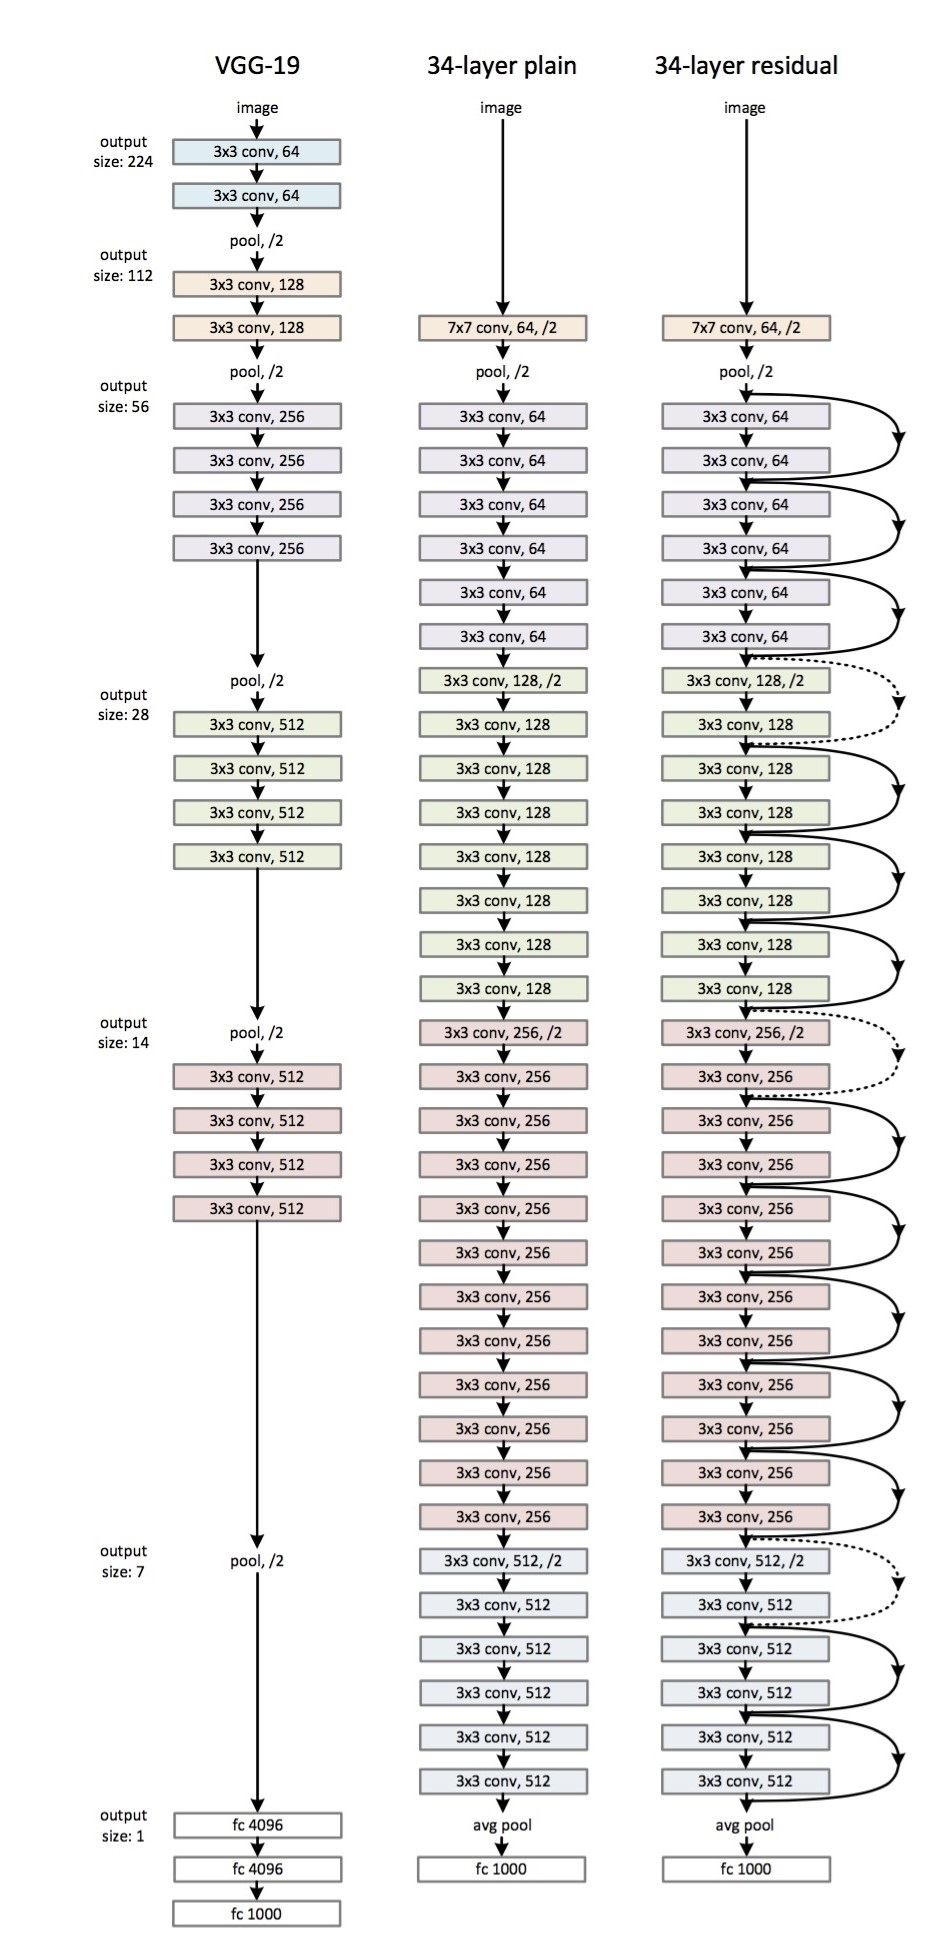
\includegraphics[width=1.0\textwidth, height=1.3\textwidth]{img/c4/resnet-34.jpg}
    \caption{ResNet-34 compared with VGG-19 and 34-layer plain network.}
    \label{resnet-34}
\end{figure}

In ResNet-34:

\begin{itemize}
    \item All the $3\times 3$ Conv are same Convs.
    \item Keep it simple in design of the network.
    \item Spatial Size / 2 $\to$ Number of filters * 2.
    \item No FC layers, no dropout is used.
    \item Two main types of blocks are used in a ResNet, depending mainly on whether the input/output dimensions are same or different. You are going to implement both of them.
    \item The dotted lines is the case when the dimensions are different. To solve then they down-sample the input by 2 and then pad zeros to match the two dimensions. There's another trick which is called bottleneck which we will explore later.
\end{itemize}

\subsubsection{Residual Block Types}
\paragraph{Identity Block}
Here is the identity block (Fig. \ref{identity-block}):

\begin{figure}[!htbp]
    \centering
    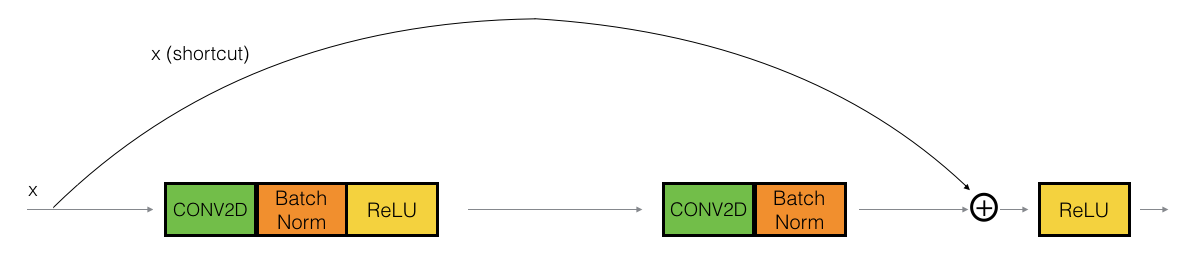
\includegraphics[width=1.0\textwidth]{img/c4/identity-block.png}
    \caption{Identity block.}
    \label{identity-block}
\end{figure}

The Conv is followed by a batch norm before ReLU. Dimensions here are same.

This skip is over 2 layers. The skip connection can jump n connections where n>2.

\paragraph{Convolutional Block} Here is the convolutional block (Fig. \ref{convolutional-block}):

\begin{figure}[!htbp]
    \centering
    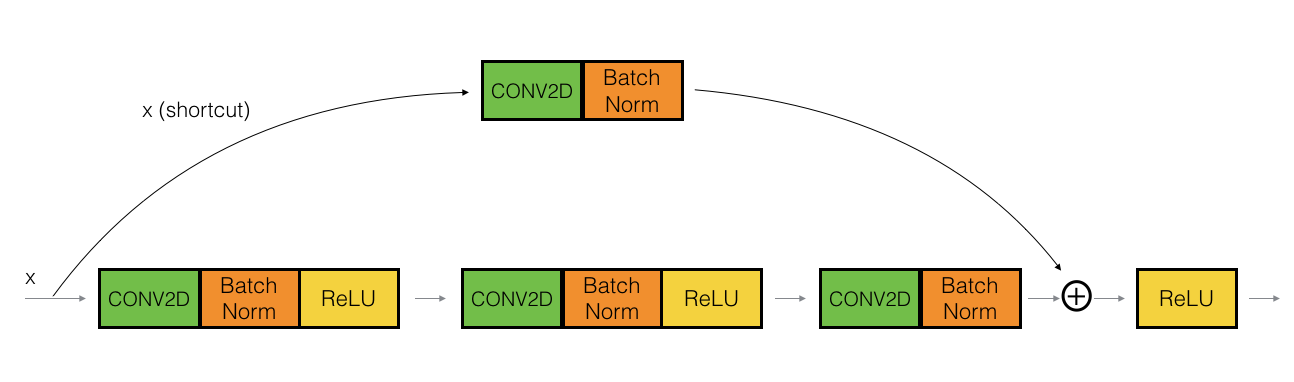
\includegraphics[width=1.0\textwidth]{img/c4/conv-block.png}
    \caption{Convolutional block.}
    \label{convolutional-block}
\end{figure}

The Conv can be bottleneck $1\times 1$ Conv.

\subsubsection{Network in Network and 1 Times 1 Convolutions}
A $1\times 1$ convolution - a very important operation in Network in Network \cite{lin2013network}- is very useful in many CNN modes.

A $1\times 1$ convlution is useful when: 
\begin{itemize}
    \item We want to shrink the number of channels. We also call this feature transformation.
    \item Save computations.
    \item If we have specified the number of 1 x 1 Conv filters to be the same as the input number of channels then the output will contain the same number of channels. Then the 1 x 1 Conv will act like a non linearity and will learn non linearity operator.
\end{itemize}

\subsubsection{Inception Network Motivation}
When you design a CNN you have to decide all the layers yourself. You may pick a $3\times 3$ Conv or $5\times 5$ Conv or maybe a max pooling layer. You have so many choices.

What \textbf{Inception} tell us is, why not use all of them at one?

Inception module \cite{szegedy2015going}, naive version (Fig. \ref{inception-naive}):

\begin{figure}[!htbp]
    \centering
    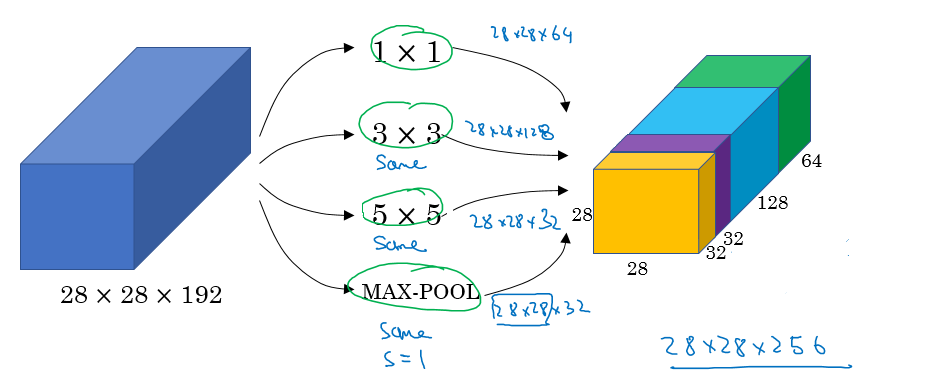
\includegraphics[width=1.0\textwidth]{img/c4/inception-naive.png}
    \caption{Inception module, naive version.}
    \label{inception-naive}
\end{figure}

Max-pool is 'SAME' here.

Input to the inception module is $28\times 28\times 192$ and the output is $28\times 28\times 256$.

We have done all the Convs and pools we might want and will let the NN learn and decide which it want to use most.

% The problem of computational cost in Inception model:

% \begin{itemize}
%     \item 
% \end{itemize}

There is high computational cost in Inception model especially for convolution operations with big kernel size. However, we can use $1\times 1$ convolution to reduce the total number of multiplications.

A $1\times 1$ Conv here is called Bottleneck. It turns out that $1\times 1$ Conv won't hurt the performance.

Inception module, dimensions reduction version (Fig. \ref{inception-reduced}):

\begin{figure}[!htbp]
    \centering
    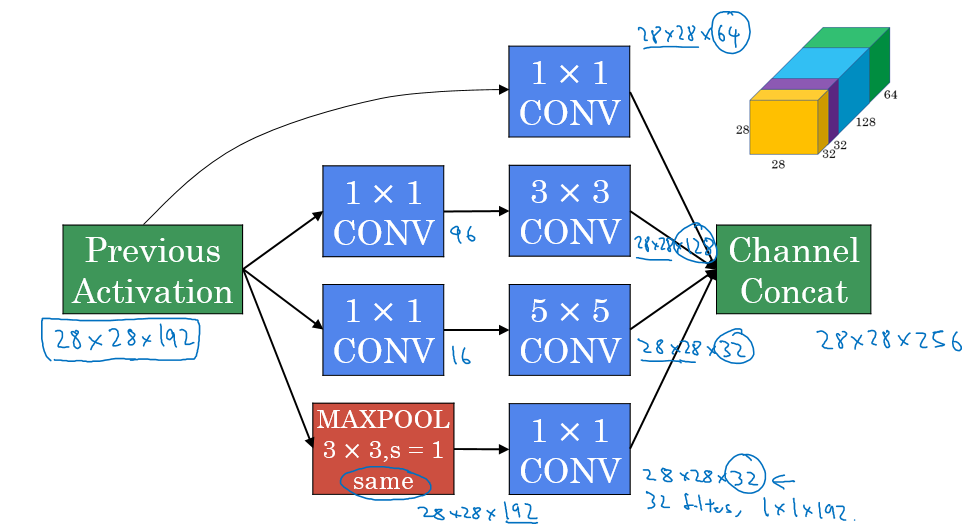
\includegraphics[width=0.9\textwidth]{img/c4/inception-reduced.png}
    \caption{Inception module, dimensions reduction version.}
    \label{inception-reduced}
\end{figure}

Example of inception model in Keras (Figure \ref{inception-keras}):

\begin{figure}[!htbp]
    \centering 
    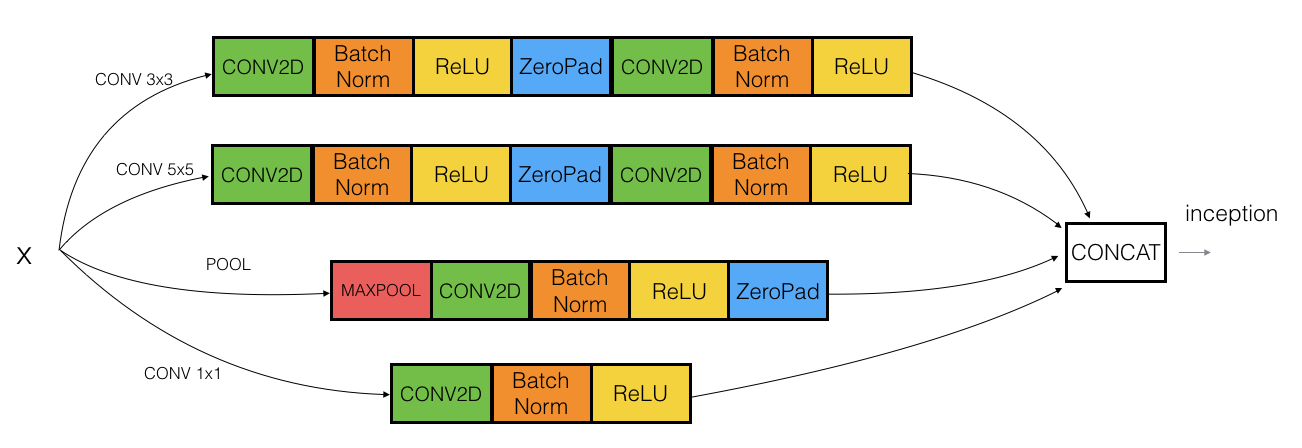
\includegraphics[width=1.0\textwidth]{img/c4/inception_keras.png}
    \caption{Inception module in Keras}
    \label{inception-keras}
\end{figure}

\subsubsection{Inception Network (GoogLeNet)}
The inception network consist of concatenated blocks of the Inception module.

The full model of GoogLeNet \cite{szegedy2015going} can be found at \href{https://nbviewer.jupyter.org/github/mbadry1/DeepLearning.ai-Summary/blob/master/4-\%20Convolutional\%20Neural\%20Networks/Images/15.png}{Here} (Also Figure \ref{googlenet}):

% Replace it with a new url.

\begin{figure}[!htbp]
    \centering 
    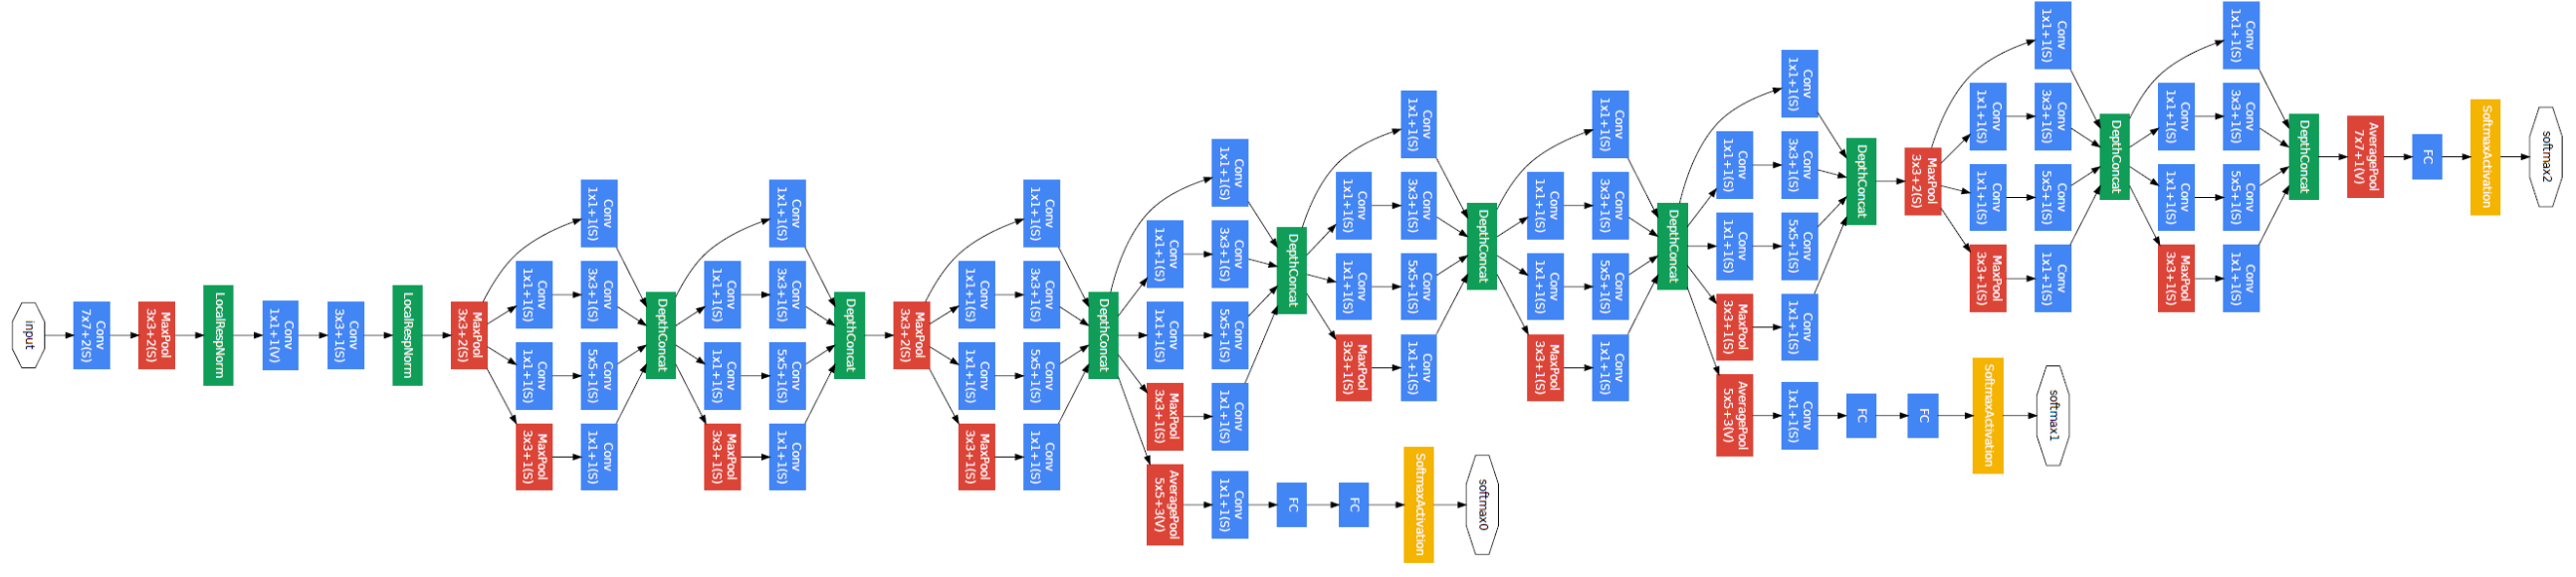
\includegraphics[width=1.1\textwidth, trim={0 0 0 0}, clip]{img/c4/google-net2.png}
    \caption{GoogLeNet architecture.}
    \label{googlenet}
\end{figure}

Some times a max-pool block is used before the inception module to reduce the dimensions of the inputs.

There are 3 softmax branches at different positions to push the network toward its goal, and helps to ensure that the intermediate features are good enough to the network and it turns out that softmax0 and softmax1 gives regularization effect.

Since the development of the Inception module, the authors and the others have built another versions of this network. Like inception v2, v3, and v4. Also there is a network that has used the inception module and the ResNet together.

\subsubsection{Transfer Learning}
If you're using a specific NN architecture that has been trained before, you can use this pretained parameters/weights instead of random initialization to solve your problem.

It can help you boost the performance of the NN.

The pretrained models might have trained on a large dataset like ImageNet or COCO and took a lot of time to learn those parameters/weights with optimized hyperparameters. This can save you a lot of time (parameters freezing technique).

\subsubsection{Data Augmentation}
If data is increased, your deep NN will perform better. Data augmentation is one of the technique that deep learning uses to increase the performance of deep NN.

The majority of computer vision applications needs more data right now.

Some data augmentation methods that are used for computer vision tasks includes:

\begin{itemize}
    \item Mirroring.
    \item Random cropping.
    \begin{itemize}
        \item The issue with this technique is that you might take a wrong crop.
        \item The solution is to make your crops big enough.
    \end{itemize}
    \item Rotation.
    \item Shearing.
    \item Local warping.
    \item Color shifting.
    \begin{itemize}
        \item For example, we add to R, G, and B some distortions that will make the image identified as the same for the human but is different for the computer.
        \item In practice the added value are pulled from some probability distribution and these shifts are some small.
        \item Makes your algorithm more robust in changing colors in images.
        \item There are an algorithm which is called \textbf{PCA color augmentation} that decides the shifts needed automatically.
    \end{itemize}
\end{itemize}

Implementing distortions during training:

You can use a different CPU thread to make you a distorted mini batches while you are training your NN.

Data Augmentation has also some hyperparameters. A good place to start is to find an open source data augmentation implementation and then use it or fine tune these hyperparameters.

Tips for doing well on benchmarks/winning competitions:

I). Ensembling.
\begin{itemize}
    \item Train several networks independently and average their outputs. Merging down some classifiers.
    \item After you decide the best architecture for your problem, initialize some of that randomly and train them independently.
    \item This can give you a push by 2\%.
    \item But this will slow down your production by the number of the ensembles. Also it takes more memory as it saves all the models in the memory.
    \item People use this in competitions but few uses this in a real production.
\end{itemize}

II). Multi-crop at test time.
\begin{itemize}
    \item Run classifier on multiple versions of test versions and average results.
    \item There is a technique called 10 crops that uses this.
    \item This can give you a better result in the production.
\end{itemize}


\subsection{Object Detection}
The aim of this section is to learn how to apply your knowledge of CNNs to one of the toughest but hottest field of computer vision: object detection.

\subsubsection{Object Localization}
What are localization and detection?

\paragraph{Image Classification} Classify an image to a specific class. The whole image represents one class. We don't want to know exactly where is the object. usually one object is presented.

\paragraph{Classfication With Localization} Given an image we want to learn the class of the image and where is the class location in the image. We need to detect a class and a rectangle of where the object is. Usually only one object is presented.

\paragraph{Object Detection} Given an image we want to detect all the object in the image that belong to a specific classes and give their location. An image can contain more than one object with different classes.

\paragraph{Semantic Segmentation} We want to label each pixel in the image with a category label. Semantic segmentation don't differentiate instances, only care about pixels. It detects no objects just pixels.

If there are two objects of the same class is intersected, we won't be able to separate them.

\paragraph{Instance Segmentation} This is like the full problem. Rather than we want to predict the bounding box, we want to know which pixel label but also distinguish them.

To make image classification we use a ConvNet with a softmax attached to the end of it.

The make classification with localization we use a ConvNet with a softmax attached to the end of it and a four numbers bx, by, bh and bw to tell you the location of the class in the image. The dataset should contain this four numbers with the class too.

\subsubsection{Landmark Detection}
In some of the computer vision problems, you will need to output some points. That is called \textbf{landmark detection}.

For example, if you're working on a face recognition problem you might want some points on the face like corners of the eyes, corners of the mouth, and corners of the nose and so on. This can help in a lot of application like detecting the pose of the face.

Y shape for the face recognition problem that needs to output 64 landmarks:

\begin{lstlisting}[language=python]
Y = [
        ThereIsAface   # Probability of face is presented 0 or 1
        l1x,
        l1y,
        ....,
        l64x,
        l64y
]
\end{lstlisting}

Another application is when you need to get the skeleton of the person using different landmarks/points in the person which helps in some applications.

In your labeled data, if l1x,l1y is the left corner of left eye, all other l1x,l1y of the other examples has to be the same.

\subsubsection{Object Detection}
We will use a ConvNet first to solve the object detection problem using a technique caleed the sliding windows detection algorithm.

For example, let's say we're working on Car object detection.

The first thing, we will train a ConvNet on cropped car images and nor car images. After we finish feeding this ConvNet with data, we will then use it with the sliding windows technique.

% Continue from here: https://github.com/mbadry1/DeepLearning.ai-Summary/tree/master/4-%20Convolutional%20Neural%20Networks#object-detection-1

Sliding windows detection algorithm:
\begin{itemize}
    \item[i.] Decide a rectangle size.
    \item[ii.] Split your image rectangles of the size you picked. Each region should be covered. You can use some strides.
    \item[iii.] For each rectangle feed the image into the ConvNet and decide if its a car or not.
    \item[iv.] Pick larger/smaller rectangles and repeat the process from ii. to iii.
    \item[v.] Store the rectangles that contains the cars.
    \item[vi.] If two or more rectangles intersects choose the rectangle with the best accuracy.
\end{itemize}

Disadvantage of sliding window is the computation time.

In the era of machine learning before deep learning, people used a hand crafted linear classifiers that classifies the object and then use the sliding window technique. The linear classifier makes it a cheap computation. But in the deep learning era that is so computational expensive due to the complexity of the deep learning model.

To solve this problem, we can implement the sliding windows with a \textbf{Convolutional approach}.

One other idea is to compress your deep learning model.

\subsubsection{Convolutional Implementation of Sliding Windows}
Turning FC layer into convolutional layers (predict image class from four classes) (Figure \ref{sliding-window}):

\begin{figure}[!htbp]
    \centering
    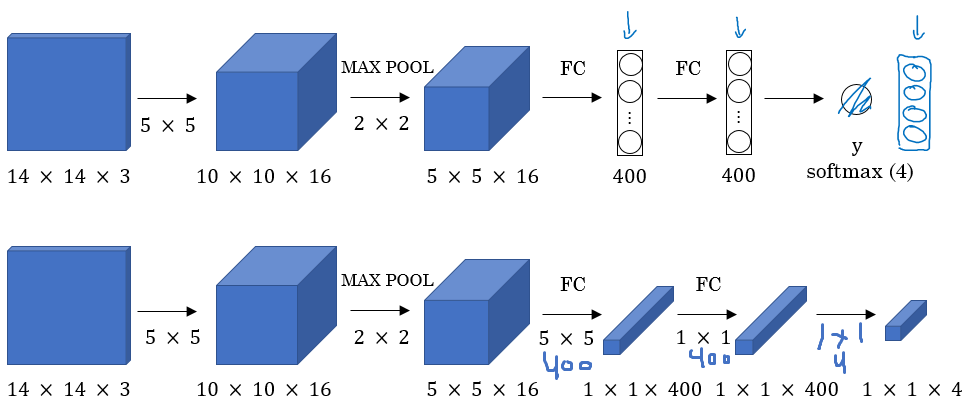
\includegraphics[width=1.0\textwidth]{img/c4/sliding-window.png}
    \caption{Convolutional implementation of sliding windows.}
    \label{sliding-window}
\end{figure}

As you can see in the above image, we turned the FC layer into a Conv layer using a convolution with the width and height of the filter which is the same as the width and height of the input.

The convolution implementation of sliding windows:

\begin{itemize}
    \item First lets consider that the Conv net you trained is like this (Figure \ref{sliding-window2}. No FC all is Conv layers.)
    \begin{figure}[!htbp]
        \centering
        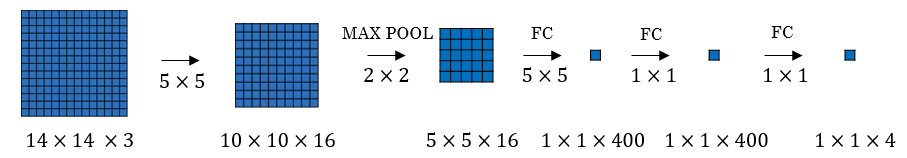
\includegraphics[width=1.0\textwidth]{img/c4/sliding-window2.png}
        \caption{Convolutional implementation of sliding windows (Visualization).}
        \label{sliding-window2}
    \end{figure}
    \item Say now we have a $16\times 16\times 3$ image that we need to apply the sliding windows in. By the normal implementation that has been mentioned in the section before, we would run this Conv net four times each rectangle size will be $14\times 14$.
    \item The convolution implementation will be as follows:
        \begin{figure}[!htbp]
            \centering
            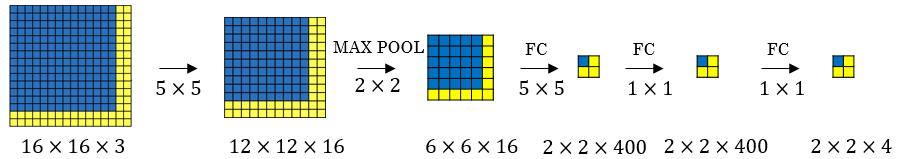
\includegraphics[width=1.0\textwidth]{img/c4/sliding-window3.png}
            \caption{Convolutional implementation of sliding windows (Visualization).}
            \label{sliding-window3}
        \end{figure}
    \item The left cell of the result "blue one" will represent the first sliding window of the normal implementation. The other cells will represent the others.
    \item Its more efficient because it now shares the computations of the four times needed.
\end{itemize}

The weakness of the algorithm is that the position of the rectangle won't be so accurate. Maybe none of the rectangles is exactly on the object you want to recognize (Figure \ref{fail2recognize}).

\begin{figure}[!htbp]
    \centering
    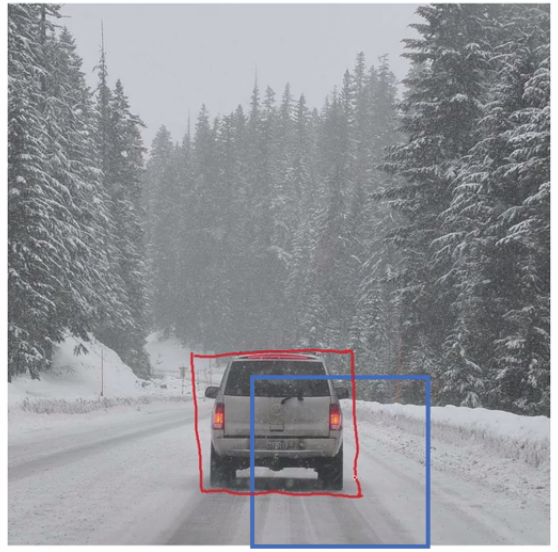
\includegraphics[width=1.0\textwidth, trim={0 0 0 200}, clip]{img/c4/fail2recognize.png}
    \caption{A failure example of convolutional sliding window algorithm.}
    \label{fail2recognize}
\end{figure}

The rectangle in red is what we want while the rectangle in blue is what the algorithm outputs.

\subsubsection{Bounding Box Predictions}
A better algorithm than the convolutional sliding windows in the last section is the YOLO algorithm \cite{redmon2016you}. 

YOLO algorithm (Figure \ref{yolo1}):

\begin{figure}[!htbp]
    % \flushleft
    \centering
    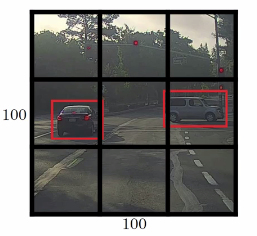
\includegraphics[width=0.5\textwidth, trim={0 0 0 0}, clip]{img/c4/yolo1.png}
    \caption{Example of YOLO algorithm.}
    \label{yolo1}
\end{figure}

\begin{itemize}
    \item Lets say we have an image of $100\times 100$.
    \item Place a $3\times 3$ grid on the image. For more smother results you should use $19\times 19$ for the $100\times100$.
    \item Apply the classification and localization algorithm we discussed in a previous section to each section of the grid. $bx$ and $by$ represent the center point of the object in each grid and will be relative to the box so the range is between 0 and 1 while $bh$ and $bw$ will represent the height and width of the object which can be greater than 1.0 but still a floating point value.
    \item Do everything at once with the convolution sliding window. If Y shape is $1\times8$ as we discussed before then the output of the $100\times 100$ image should be $3\times 3\times 8$ which corresponds to $9$ cell results.
    \item Merging the results using predicted localization mid point.
\end{itemize}

We have a problem if we have found more than one object in one grid box.

One of the best advantages that makes the YOLO algorithm popular is that it has a great speed and a Conv net implementation.

How is YOLO different from other Object detectors? YOLO uses a single CNN network for both classification and localizing the object using bounding boxes.

In the next section we will see some ideas that can make the YOLO algorithm better.

\subsubsection{Intersection Over Union}
Intersection Over Union (IoU) is a function used to evaluate the object detection algorithm. It computes the size of intersection and divide it by the union. More generally, IoU is a measure of the overlap between two bounding boxes.

\subsubsection{Non-Max Suppression}
One of the problems we have addressed in YOLO is that it can detect an object multiple times. Non-max suppression is a way to make sure that YOLO detects the object just one.

For example \ref{nms}:

\begin{figure}[!htbp]
    % \flushleft
    \centering
    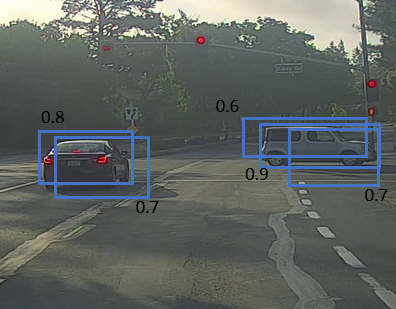
\includegraphics[width=0.5\textwidth, trim={0 0 0 0}, clip]{img/c4/nms.png}
    \caption{Non-max suppression.}
    \label{nms}
\end{figure}

Each car has two or more detections with different probabilities. This came from some of the grids that thinks that this is the center point of the object.

Non-max suppression algorithm:

\begin{itemize}
    \item Lets assume that we are targeting one class as an output class.
    \item Y shape should be $[P_c, b_x, b_y, b_h, b_w]$. Where $P_c$ is the probability if that object occurs.
    \item Discard all boxes with $P_c < 0.6$.
    \item While there are any remaining boxes:
    \begin{itemize}
        \item[i.] Pick the box with the largest $P_c$ output that as a prediction.
        \item[ii.] Discard any remaining box with $IoU > 0.5$ with that box output in the previous step. i.e. any box with high overlap (greater than overlap threshold of 0.5).
    \end{itemize}
\end{itemize}

If there are multiple classes types c you want to detect, you should run the non-max suppression c times, once for every output class.

\subsubsection{Anchor Boxes}
In YOLO, a grid only detects one object. What if a grid cell wants to detect multiple object?

\begin{figure}[!htbp]
    % \flushleft
    \centering
    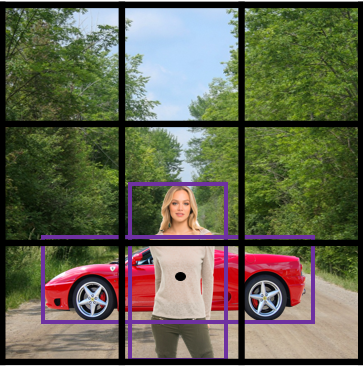
\includegraphics[width=0.5\textwidth, trim={0 0 0 0}, clip]{img/c4/yolo3.png}
    \caption{Example of anchor boxes.}
    \label{anchor}
\end{figure}

As we can see from Figure \ref{anchor}, car and person grid is same here. In practice this actually happens rarely. 

The idea of anchor boxes helps us solving this issue.

If $Y = [Pc, bx, by, bh, bw, c1, c2, c3]$. Then to use two anchor boxes like this:

\begin{itemize}
    \item $Y = [Pc, bx, by, bh, bw, c1, c2, c3, Pc, bx, by, bh, bw, c1, c2, c3]$. We simply have repeated the one anchor Y.
    \item The two anchor boxes you choose should have known shape (Figure \ref{anchor2}):
    \begin{figure}
        \centering
        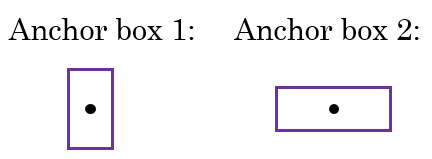
\includegraphics[width=0.6\textwidth]{img/c4/anchor2.png}
        \caption{Visualization of two anchor boxes.}
        \label{anchor2}
    \end{figure}
\end{itemize}

With no anchor box, each object in training image is assigned to grid cell that contains that object's midpoint. With two anchor boxes, each object in training image is assigned to grid cell that contains object's midpoint and anchor box for the grid cell with highest IoU. We suppose that every object detected is similar to an anchor box which has similar shape.

You may have two or more anchor boxes but you should know their shapes.

\begin{itemize}
    \item How do you choose the anchor boxes and people used to just choose them by hand. Maybe five or ten anchor box shapes that spans a variety of shapes that cover the types of objects you seem to detect frequently.
    \item You may also use a k-means algorithm on your dataset to specify that.
\end{itemize}

Anchor boxes allows your algorithm to specialize, means in our case to easily detect wider images or taller ones.

\subsubsection{YOLO Algorithm}
Suppose we need to do object detection for our autonomous driving system. It needs to identify three classes: Pedestrain, Car and Motorcycle.

We decided to choose two anchor boxes, a tall one and a wide one. (Like we said in practice they use five or more anchor boxes hand made or generated using k-means.)

Our labeled Y shape will by $[Ny, HeightOfGrid, WidthOfGrid, 16]$, where $Ny$ is the number of instances and each row is as follows:

\begin{itemize}
    \item $[Pc, bx, by, bh, bw, c1, c2, c3, Pc, bx, by, bh, bw, c1, c2, c3]$
\end{itemize}

Your dataset could be an image with a multiple labels and a rectangle for each label. For example (Figure \ref{yolo2}):

\begin{figure}
    \centering
    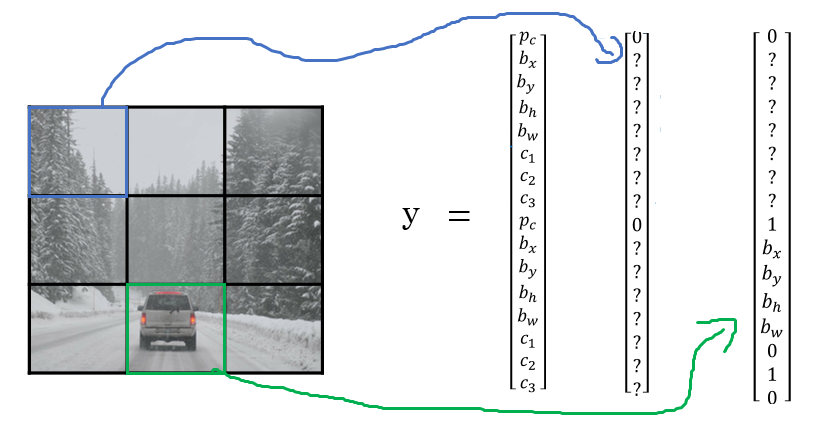
\includegraphics[width=0.8\textwidth]{img/c4/yolo2.png}
    \caption{An extension example of YOLO Ny.}
    \label{yolo2}
\end{figure}

\begin{itemize}
    \item We first initialize all of them to zeors and ?, then for each label and rectangle choose its closest grid point then the shape to fill it and then the best anchor point based on the IoU, so that the shape of Y for one image should be $[HeightOfGrid, WidthOfGrid,16]$.
\end{itemize}

Train the labeled images on a Conv net, you should receive an output of $[HeightOfGrid, WidthOfGrid,16]$ of our case.

To make predictions, run the Conv net on an image and run non-max suppression algorithm for each class you have. In our case, there are 3 classes (Figure \ref{yolo4}). Total number of generated boxes are grid\_width * grid\_height * num\_anchors = $3\times 3 \times 2$. By removing the low probability predictions you should have (Figure \ref{yolo5}). Then get the best probability followed by the IoU filtering (Figure \ref{yolo6}). The details network set up could refer to \href{https://github.com/mbadry1/DeepLearning.ai-Summary/tree/master/4-\%20Convolutional\%20Neural\%20Networks#yolo-algorithm}{Github}.

\begin{figure}[!htbp]
\begin{subfigure}{.33\textwidth}
  \centering
  % include first image
  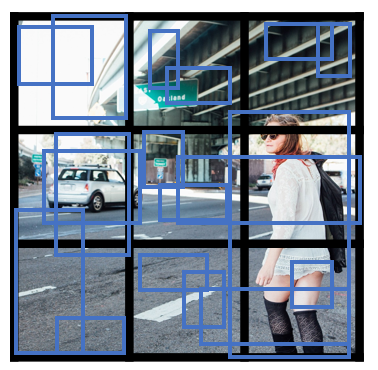
\includegraphics[width=1.0\linewidth]{img/c4/yolo4.png}  
  \caption{Predicted anchor boxes.}
  \label{yolo4}
\end{subfigure}
\begin{subfigure}{.33\textwidth}
  \centering
  % include second image
  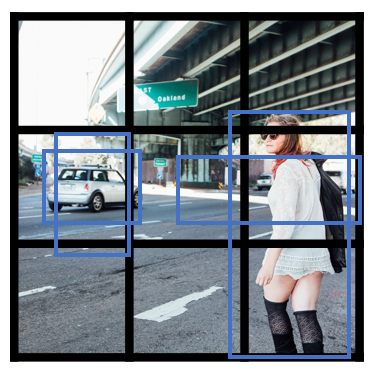
\includegraphics[width=1.0\linewidth]{img/c4/yolo5.png}  
  \caption{Predicted anchor boxes (removing low probability predictions).}
  \label{yolo5}
\end{subfigure}
\begin{subfigure}{.33\textwidth}
  \centering
  % include third image
  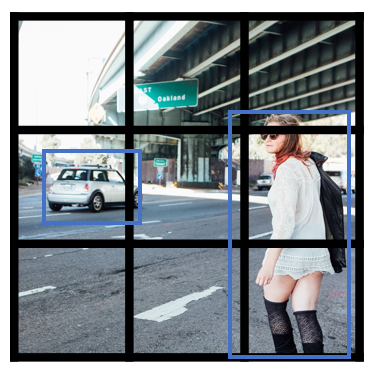
\includegraphics[width=1.0\linewidth]{img/c4/yolo6.png}
  \caption{Predicted anchor boxes (removing low probability predictions and using IoU filtering).}
  \label{yolo6}
\end{subfigure}
\end{figure}

\subsubsection{Region Proposals (R-CNN)}
YOLO is fast but the downside of it is that it process a lot of areas where no objects are presented. R-CNN tries to pick a few windows and run a Conv net (your confident classifier) on top of them.

The algorithm R-CNN \cite{girshick2014rich} uses to pick windows is called a segmentation algorithm. Outputs something like this (Figure \ref{rcnn1}):

\begin{figure}
    \centering
    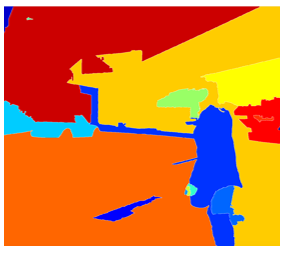
\includegraphics[width=0.6\textwidth]{img/c4/rcnn1.png}
    \caption{Segmentation result by using R-CNN to pick windows.}
    \label{rcnn1}
\end{figure}

If for example the segmentation algorithm produces 2000 blob then we should run our classifier/CNN on top of these blobs.

There has been a lot of work regarding R-CNN tries to make it faster:

\begin{itemize}
    \item R-CNN\cite{girshick2014rich}: Propose regions. Classify proposed regions one at a time. Output label + bounding box. Downside is that it's slow.
    \item Fast R-CNN\cite{girshick2015fast}: Propose regions. Use convolution implementation of sliding windows to classify all the proposed regions.
    \item Faster R-CNN\cite{ren2015faster}: Use convolutional network to propose regions.
    \item Mask R-CNN\cite{he2017mask}.
\end{itemize}

Most of the implementations of faster R-CNN are still slower than YOLO. Andrew Ng thinks that the idea behind YOLO is better than R-CNN because you're able to do all the things in just one stage instead of two stages.


\subsection{Face Recognition}
% \subsection{Special Applications: Face Recognition and Neural Style Transfer}
This section and the next section are aimed at discovering how CNNs can be applied to multiple fields, including art generation and face recognition. Besides, try to implement you own algorithm to generate art and recognize faces. So first we will talke about face recognition.

\subsubsection{What Is Face Recognition?}
Face recognition system identifies a person's face. It can work on both images or videos.

Face verification vs. face recognition:

\begin{itemize}
    \item Verification:
    \begin{itemize}
        \item Input: image, name/ID. (1:1)
        \item Output: whether the input image is that of the claimed person.
        \item "Is this the claimed person?"
    \end{itemize}
    \item Recognition:
    \begin{itemize}
        \item Has a database of K persons and get an input image.
        \item Output ID if the image is any of the K persons (or not recognized).
        \item "Who is this person?"
    \end{itemize}
\end{itemize}

We can use a face verification system to make a face recognition system. The accuracy of the verification system has to be high (around 99.9\% or more) to be use accurately within a recognition system because the recognition system accuracy will be less than the verification system given K persons.

\subsubsection{One-Shot Learning}
One of the face recognition challenges is to solve one shot learning problem.

One Shot Learning: A recognition system is able to recognize a person, learning from one image.

Historically deep learning doesn't work well with a small number of data.

Instead to make this work, we will learn a \textbf{similarity function}:
\begin{itemize}
    \item d(img1, img2) = degree of difference between images.
    \item We want d result to be low in case of the same faces.
    \item We use $\tau$ as a threshold for d: if d(img1, img2) $\leq \tau$, then the faces are the same.
\end{itemize}

Similarity function helps us solving the one shot learning. Also its robust to new inputs.

\subsubsection{Siamese Network}
We will implement the similarity function using a type of NNs called Siamese Network \cite{koch2015siamese} in which we can pass multiple inputs to the two or more networks with the same architecture and parameters.

Siamese network architecture is as the following (Figure \ref{siamese}):

\begin{figure}[!htbp]
    \centering
    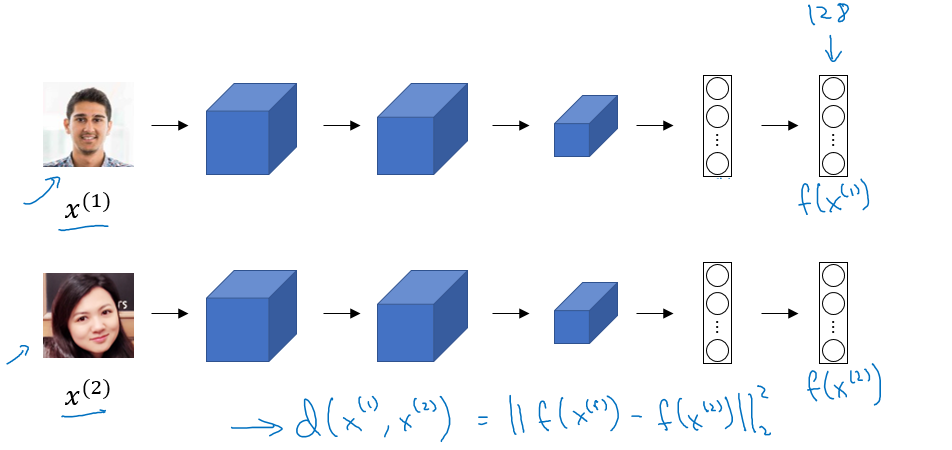
\includegraphics[width=1.0\textwidth]{img/c4/siamese.png}
    \caption{Siamese network.}
    \label{siamese}
\end{figure}

We make 2 identical ConvNets which encoders an input image into a vector. In the above image the vector shape is (128,). 

The loss function will be $d(x1, x2) = ||f(x1) - f(x2)||^2$.

If x1 and x2 are the same person, we want d to be low. If they are different persons, we want d to be high.

\subsubsection{Triplet Loss}
Triplet loss is one of the loss functions we can use to solve the similarity distance in a Siamese Network.

Our learning objective in the triplet loss function is to get the distance between an \textbf{anchor} image and a positive or a negative image (positive means same person, while negative means different person).

The triplet name came from that we are comparing an anchor A with a positive P and a negative N image.

Formally we want:

\begin{itemize}
    \item Positive distance to be less than negative distance: $||f(A)-f(P)||^2 \leq ||f(A) - f(N)||^2$.
    \item Then $||f(A)-f(P)||^2 - ||f(A) - f(N)||^2 \leq 0$.
    \item To make sure the NN won't get an output of zeros easily: $||f(A)-f(P)||^2 - ||f(A) - f(N)||^2 \leq -\alpha$. $\alpha$ is a small number. Sometimes its called the margin.
    \item Then $||f(A)-f(P)||^2 - ||f(A) - f(N)||^2 + \alpha \leq 0$. 
\end{itemize}

Final loss function:
\begin{itemize}
    \item Given 3 images (A, P, N)
    \item $L(A, P, N) = \max (||f(A)-f(P)||^2 - ||f(A) - f(N)||^2 + \alpha, 0)$.
    \item $J = \sum(L(A[i], P[i], N[i]))$ for all triplets of images.
\end{itemize}

You need multiple images of the same person in your dataset. Then get some triplets out of your dataset. Dataset should be big enough.

Choosing the triplets A, P, N:

\begin{itemize}
    \item During training, if A, P, N are chosen randomly (subject to A and P are the same and A and N aren't the same), then one of the problems is the following constrain is easily satisfied ($d(A, P) + \alpha \leq d(A, N)$). So the NN won't learn much.
    \item What we want to do is to choose triplets that are hard to train on. So for all the triplets we want the above equation to be satisfied. Details are in FaceNet\cite{schroff2015facenet}.
\end{itemize}

\subsubsection{Face Verification and Binary Classification}
Triplet loss is one way to learn the parameters of a ConvNet for face recognition. However, there's another way to learn these parameters as a straight binary classification problem.

Learning the similarity function another way\cite{taigman2014deepface} (Figure \ref{triplet-loss}):

\begin{figure}[!htbp]
    \centering
    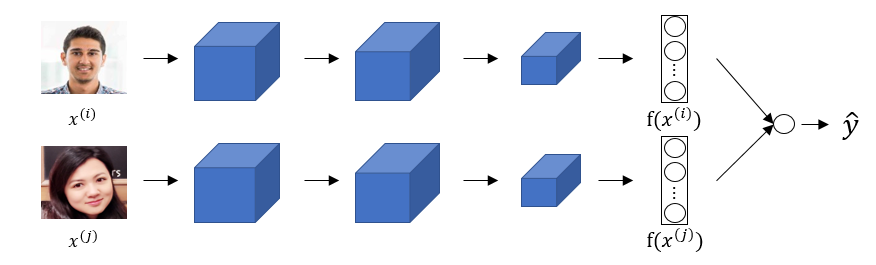
\includegraphics[width=1.0\textwidth]{img/c4/triplet-loss.png}
    \caption{Learning the similarity function in one network.}
    \label{triplet-loss}
\end{figure}

\begin{itemize}
    \item The final layer is a sigmoid layer.
    \item $\hat{Y} = w_{ij} sigmoid (f(x_i) - f(x_j)) + b$, where the substraction is the Manhattan distance between $f(x_i)$ and $(f(x_j)$.
    \item Some other similarities can be Euclidean distance similarity.
\end{itemize}

A good performance/deployment trick:
\begin{itemize}
    \item Pre-compute all the images that you're using as a comparison to the vector $f(x_j)$.
    \item When a new image that needs to be compared, get its vector $f(x_i)$ then put it with all the pre-computed vectors and pass it to the sigmoid function.
\end{itemize}

This version works quite as well as the triplet loss function.

\subsection{Neural Style Transfer}
\subsubsection{What Is Neural Style Transfer?}
Neural style transfer takes a content image $c$ and a style image $s$ and generates the content image $g$ with the style of style image. e.g. Figure \ref{style-transfer}.

\begin{figure}[!htbp]
    \centering
    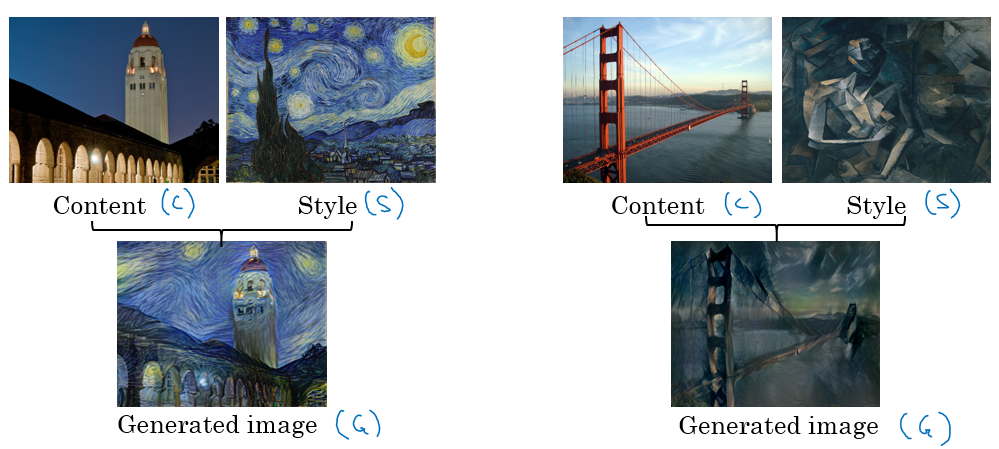
\includegraphics[width=1.0\textwidth]{img/c4/style-transfer.png}
    \caption{Examples of neural style transfer.}
    \label{style-transfer}  
\end{figure}

In order to implement this you need to look at the features extracted by the ConvNet at the shallower and deeper layers.

It uses a previously trained convolutional network like VGG, and builds on top of that. The idea of using a network trained on a different task and applying it to a new task is called transfer learning.

\subsubsection{What Is Deep ConvNets Learning?}
Visualizing what a deep network is learning. Firstly, give this AlexNet like ConvNet (Figure \ref{visualize-convs}).

\begin{figure}[!htbp]
    \centering
    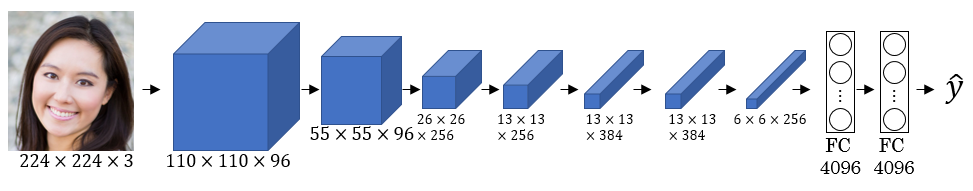
\includegraphics[width=1.0\textwidth]{img/c4/visualize-convnets.png}
    \caption{AlexNet like ConvNet.}
    \label{visualize-convs}  
\end{figure}

Pick a unit in layer l. Find the nine image patches that maximize the unit's activation. Notice that a hidden unit in layer 1 will see relatively small portion of NN, so if you plotted it it will match a msall image in the shallower layers while it will get larger image in deeper layers.

Repeating for other units and layers.

It turns out that layer 1 is learning the low level representations like colors and edges.

You will find out that deeper layers are learning more complex representations\cite{zeiler2014visualizing} (Figure \ref{visualize-convs2}).

\begin{figure}[!htbp]
    \centering
    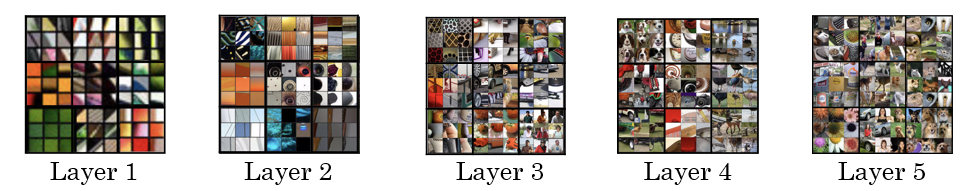
\includegraphics[width=1.0\textwidth]{img/c4/visualize-convnets2.png}
    \caption{Visualization of ConvNets.}
    \label{visualize-convs2}  
\end{figure}

A good explanation on how to get receptive field given a layer\footnote{https://medium.com/mlreview/a-guide-to-receptive-field-arithmetic-for-convolutional-neural-networks-e0f514068807} (Figure \ref{receptivefield}):

\begin{figure}[!htbp]
    \centering
    \includegraphics[width=1.0\textwidth]{img/c4/receptiveField.png}
    \caption{An explanation of how to get receptive field.}
    \label{receptivefield}  
\end{figure}  

% not very familiar with how to calculate receptive field.

\subsubsection{Cost Function}
We will define a cost function for the generated image that measures how good it is.

Given a content image C, a style image S, and a generated image G:
\begin{itemize}
    \item $J(G) = \alpha J(C, G) + \beta J(S, G)$
    \item $J(C, G)$ measures how similar is the generated image to the content image.
    \item $J(S, G)$ measures how similar is the generated image to the style image.
    \item $\alpha$ and $\beta$ are relative weighting to the similarity and these are hyperparameters.
\end{itemize}

Find the generated image G:

\begin{itemize}
    \item[i.] Initialize G randomly.
    \item[ii.] Use gradient descent to minimize $J(G)$. $G = G - dG$. We compute the gradient image and use gradient descent to minimize the cost function.
\end{itemize}

The iterations might be as following image:

To generate by using the following (Figure \ref{cgimage}):

\begin{figure}[!htbp]
    \centering
    \includegraphics[width=1.0\textwidth]{img/c4/cgimage.png}
    \caption{Provided content image C and style image G.}
    \label{cgimage}  
\end{figure}  

You will go through this (Figure \ref{stagedG}):
\begin{figure}[!htbp]
    \centering
    \includegraphics[width=1.0\textwidth]{img/c4/stagedG.png}
    \caption{Staged pictures of generated image G.}
    \label{stagedG}  
\end{figure}  

\subsubsection{Content Cost Function}
In the previous section we showed that we need a cost function for the content image and the style image to measure how similar is them to each other.

Say you use hidden layer $l$ to compute content cost. If we choose $l$ to be small (like layer 1), we will force the network to get similar output to the original content image. In practice $l$ is not too shallow or not too deep but in the middle.

Use pre-trained ConvNet like VGG network.

Let $a(C)[l]$ and $a(G)[l]$ be the activation of layer $l$ on the images.

If $a(C)[l]$ and $a(G)[l]$ are similar then they will have the same content:

\begin{equation}
    J(C, G) at layer l = \frac{1}{2} ||a(C)[l] - a(G)[l]||^2
\end{equation}

\subsubsection{Style Cost Function}
Meaning of the \textbf{style} of an image:

\begin{itemize}
    \item Say you're using layer $l$'s activation to measure \textbf{style}.
    \item Define style as correlation between activations across channels. That means given an activation like Figure \ref{style-cost}. How correlate is the orange channel with the yellow channel?
    \begin{figure}[!htbp]
    \centering
    \includegraphics[width=0.4\textwidth]{img/c4/style-cost.png}
    \caption{Illustration of image style.}
    \label{style-cost}  
    \end{figure}  
    \item Correlated means if a value appeared in a specific channel a specific value will appear too (depend on each other). While uncorrelated means if a value appeared in a specific channel doesn't mean that the another value will appear (not depend on each other). The correlation tells you how a components might occur or not occur together in the same image.
\end{itemize}

The correlation of style image channels should appear in the generated image channels. 

Style matrix (Gram matrix):

\begin{itemize}
    \item Let $a(l)[i, j, k]$ be the activation at layer $l$ with $i=H, j=W, k=C$.
    \item Also $G(l)(s)$ is the matrix of shape $n_C(l)\times n_C(l)$ (We call this matrix style matrix or Gram matrix). In this matrix, each cell will tell us how correlated is a channel to another channel.
    \begin{equation}
        \begin{aligned}
        G_{kk'}^{[l](S)} &= \sum^{n_H^{l}}_{i=1}\sum^{n_W^{[l}}_{j=1} a_{ijk}^{[l](S)} a_{ijk'}^{[l](S)}\\
        G_{kk'}^{[l](G)} &= \sum^{n_H^{l}}_{i=1}\sum^{n_W^{[l}}_{j=1} a_{ijk}^{[l](G)} a_{ijk'}^{[l](G)}\\
        \end{aligned}
    \end{equation}
\end{itemize}

% Not too familiar with this equations.

Steps to be made if you want to create a tensorflow model for neural style transfer.

\begin{itemize}
    \item[i.] Create an Interactive Session.
    \item[ii.] Load the content image, load the style image
    \item[iii.] Randomly initialize the image to be generated.
    \item[iv.] Load the VGG16 model
    \item[v.] Build the TensorFlow graph: 1) Run the content image through the VGG16 model and compute the content cost; 2) Run the style image through the VGG16 model and compute the style cost; 3) Compute the total cost; 4) Define the optimizer and the learning rate.
    \item[vi.] Initialize the TensorFlow graph and run it for a large number of iterations, updating the generated image at every step.
\end{itemize}

\subsubsection{Keras Tutorial}
To train and test a model in Keras there are four steps:

\begin{itemize}
    \item[i.] Create the model.
    \item[ii.] Compile the model by calling \textit{model.compile(optimizer = "...", loss = "...", metrics = ["accuracy"])}.
    \item[iii.] Train the model on train data by calling \textit{model.fit(x = ..., y = ..., epochs = ..., batch\_size = ...)}. (We can add a validation set while training too.)
    \item Test the model on test data by calling \textit{model.evaluate(x = ..., y = ...)}.
\end{itemize}

Summarize of steps in Keras: Create $\to$ Compile $\to$ Fit/Train $\to$ Evaluate/Test.

Model.summary() gives a lot of useful informations regarding your model including each layers inputs, outputs, and number of parameters at each layer.

To choose the Keras backend you should go to \$HOME/.keras/keras.json and change the file to the desired backend like Theano or Tensorflow or whatever backend you want.

After you create the model you can run it in a tensorflow session without compiling, training, and testing capabilities.

You can save your model with model\_save and load your model using model\_load This will save your whole trained model to disk with the trained weights.
\newpage
\section{Sequence Models}
This is the fifth course and last course of deep learning specialization at Coursera taught by Professor Andrew Ng. Here is my certificate after finishing this course (Fig. No, currently not earned).

\subsection{Course Overview}
According to the official site of this course, you will learning the following after you finish this course:

\begin{itemize}
    \item Understand how to build and train Recurrent Neural Networks (RNNs), and commonly-used variants such at GRUs and LSTMs.
    \item Be able to apply sequence models to natural language problems, including text synthesis.
    \item Be able to apply sequence models to audio applications, including speech recognition and music synthesis.
\end{itemize}

\subsection{Recurrent Neural Networks}
In this section, you'll learn about recurrent neural network. This type of model has been proven to perform extremely well on temporal data. It has several variants including LSTMs, GRUs and Bidirectional RNNs, which you're going to learn about in this section.

\subsubsection{Why Sequence Models}
Sequence models like RNNs and LSTMs have greatly transformed learning on sequences in the past few years.

Examples of sequence data in applications:

\begin{itemize}
    \item Speech recognition (\textit{sequence to sequence}): X$\to$ wave sequence; Y$\to$ text sequence.
    \item Music generation (\textit{one to sequence}): X$\to$ nothing or an integer; Y$\to$ wave sequence.
    \item Sentiment classification (\textit{sequence to one}): X$\to$ text sequence; Y$\to$ integer rating from one to five.
    \item DNA sequence analysis (sequence to sequence): X$\to$ DNA sequence; Y$\to$ DNA labels.
    \item Machine translation (sequence to sequence): X$\to$ text sequence (in one language); Y$\to$ texe sequence (in other language). 
    \item Video activity recognition (sequence to one): X$\to$ video frames; Y$\to$ label (activity).
    \item Name entity recognition (sequence to sequence): X$\to$ text sequence; Y$\to$ label sequence.
\end{itemize}

All of these problems with different input and output (sequence or not) can be addressed as supervised learning with label data X, Y as the training set.

The goal is given this representation for x to learn a mapping using a sequence model to then target output y as a supervised learning problem.

\subsubsection{Recurrent Neural Network Model}
Why not to use a standard network for sequence tasks? There are two problems (needs to be clarified):

% needs to be clarified.

\begin{itemize}
    \item Inputs, outputs can be different lengths in different examples. This can be solved for normal NNs by paddings with the maximum lengths but its not a good solution.
    \item Doesn't share features learned across different positions of text/sequence. Using a feature sharing NN like in CNNs can significantly reduce the number of parameters in your model. That's what we will do in RNNs.
\end{itemize}

Recurrent neural network doesn't have either of the town mentioned problems.

Lets build a RNN that solves \textbf{name entity recognition} task (Figure \ref{name-entity}):

\begin{figure}[!htbp]
    \centering
    \includegraphics[width=1.0\textwidth]{img/c5/name-enttity-task.png}
    \caption{Example of name entity recognition task.}
    \label{name-entity}
\end{figure}

We should note:

\begin{itemize}
    \item In this problem, $T_x = T_y$. In other problems where thy aren't equal, the RNN architecture may be different.
    \item $a^{<0>}$ is usually initialized with zeros, but some others may initialize it randomly in some cases.
    \item There are three weight matrices here: $W_{ax}, W_{aa}$ and $W_{ya}$ with shapes: $W_{ax}\to (n_h, n_x), W_{aa}\to (n_h, n_h), W_{ya}\to (n_y, n_h)$.
\end{itemize}

The weight matrix $W_{aa}$ is the memory the RNN is trying to maintain from the previous layers.

In the discussed RNN architecture, the current output $y^{<t>}$ depends on the previous inputs and activations. 

Let's have this example `He Said, ``Teddy Roosevelt was a great president"'. In this example Teddy is a person name but we know that from the word \textit{president} that came after Teddy not from \textit{He} and \textit{said} that were before it.

So limitation of the discussed architecture is that it can not learn from elements later in the sequence. To address this problem we will later discuss \textbf{Bidirectional RNN (BRNN)}.

Now let's discuss the forward propagation equations on the discussed architecture (Figure \ref{forward-nn}):

\begin{figure}[!htbp]
    \centering
    \includegraphics[width=1.0\textwidth]{img/c5/forward-rnn.png}
    \caption{Forward propagation of a RNN.}
    \label{forward-nn}
\end{figure}

The activation function for $a$ is usually $\tanh$ or $ReLU$ and for y depends on your task choosing some activation functions like $sigmoid$ and $softmax$. In name entity recognition task we will use sigmoid because we only have two classes.

In order to help us develop complex RNN architectures, the last equations needs to be simplified a bit (Figure \ref{simple-rnn-notations}):

\begin{figure}[!htbp]
    \centering
    \includegraphics[width=1.0\textwidth]{img/c5/simple-rnn-notations.png}
    \caption{Simplified RNN notations.}
    \label{simple-rnn-notations}
\end{figure}

$w_a$ is $w_{aa}$ and $w_{ax}$ stacked horizontally. $[a^{<t-1>}, x^{<t>}]$ is $a^{<t-1>}$ and $x^{<t>}$ stacked vertically. $w_a$ shape: $(n_h, n_h+n_x)$. $[a^{<t-1>}, x^{<t>}]$ shape: $(n_h + n_x, 1)$.

\subsubsection{Backpropagation Through Time}
Usually deep learning frameworks do backpropagation automatically for you. But it's useful to know it works in RNNs.

We will use the cross-entropy loss function:

\begin{equation}
    L^{<t>}(\hat{y}^{<t>}, y^{<t>}) = - y^{<t>}\log \hat{y}^{<t>} - (1 - y^{<t>}) \log (1 - \hat{y}^{<t>})
\end{equation}

The total loss is:

\begin{equation}
    L(\hat{y}, y) = \sum_{t=1}^{T_y} L^{<t>}(\hat{y}^{<t>}, y^{<t>})
\end{equation}

The backpropagation here is called backpropagation through time because we pass activation a from one sequence element to another like backwards in time.

% Add more content of this part.

\subsubsection{Different Types of RNNs}
Here are different types of RNNs (Figure \ref{diff-rnns}, inspired by Andrej Karpathy's blog\footnote{http://karpathy.github.io/2015/05/21/rnn-effectiveness/}):

\begin{figure}[!htbp]
    \centering
    \includegraphics[width=1.0\textwidth]{img/c5/diff-rnns.jpg}
    \caption{Different kinds of RNNs.}
    \label{diff-rnns}
\end{figure}

\subsubsection{Language Model and Sequence Generation}
\textbf{What is a language model}:
\begin{itemize}
    \item Let's say we're solving a speech recognition problem and some says a sentence that can be interpreted into two sentences: a) The apple and \textit{pair} salad; b) The apple and \textit{pear} salad.
    \item \textit{Pair} and \textit{pear} sounds exactly the same, so how would a speech recognition application choose from the two.
    \item That's where the language model comes in. It gives a probability for the two sentences and the application decides the best based on this probability.
\end{itemize}

The job of a language model is to give a probability of any given sequence of words.

\textbf{How to build language models with RNNs}
\begin{itemize}
    \item The first thing is to get a training set: a large corpus of target language text.
    \item Then tokenize this training set by getting the vocabulary and then one-hot each word.
    \item Put an end of sentence token \textit{<EOS>} with the vocabulary and include it with each converted sentence. Also, use the token \textit{<UNK>} for the unknown words.
\end{itemize}

Given the sentence ``Cats average 15 hours of sleep a day. <EOS>"

In training time we will use this (Figure \ref{language-model}):

\begin{figure}[!htbp]
    \centering
    \includegraphics[width=1.0\textwidth]{img/c5/language-model.png}
    \caption{Example of language model.}
    \label{language-model}
\end{figure}

The loss function is defined by cross-entropy loss.

To use this model:
\begin{itemize}
    \item[i.] For predicting the chance of next word, we feed the sentence to the RNN and then get the final $y^{<t>}$ hot vector and sort it by maximum probability.
    \item[ii.] For taking the probability of a sentence, we compute this: $p(y^{<1>}, y^{<2>}, y^{<3>}) = p(y^{<1>}) * p(y^{<2>} | y^{<1>}) * p(y^{<3>} | y^{<1>}, y^{<2>})$. This is simply feeding the sentence into the RNN and multiplying the probabilities (outputs).
\end{itemize}

\subsubsection{Sampling Novel Sequences}
After a sequence model is trained on a language model, to check what the model has learned you can apply it to sample novel sequence.

To be continued.

% https://github.com/mbadry1/DeepLearning.ai-Summary/tree/master/5-%20Sequence%20Models#sampling-novel-sequences
\newpage
% \input{experiments.tex}

% \input{cnn-encoder.tex}

\section*{Acknowledgements}
This note is heavily based on Prof. Andrew Ng's course at Coursera. Thanks Andrew for taking this wonderful course, I've learnt a lot from that. Besides, thanks Coursera for providing me full-funded financial aids to finish all the five courses in the specialization. Moreover, parts of the note are borrowed from Mahmoud Badry's github repository\footnote{https://github.com/mbadry1/DeepLearning.ai-Summary}. It gives me a clear panorama of what is the most important.

\bibliographystyle{unsrt}  
\bibliography{references}  %%% Remove comment to use the external .bib file (using bibtex).
%%% and comment out the ``thebibliography'' section.

% \newpage
\section*{Appendix}

\end{document}
